\documentclass[12pt]{article}\usepackage[]{graphicx}\usepackage[]{color}
%% maxwidth is the original width if it is less than linewidth
%% otherwise use linewidth (to make sure the graphics do not exceed the margin)
\makeatletter
\def\maxwidth{ %
  \ifdim\Gin@nat@width>\linewidth
    \linewidth
  \else
    \Gin@nat@width
  \fi
}
\makeatother

\definecolor{fgcolor}{rgb}{0.345, 0.345, 0.345}
\newcommand{\hlnum}[1]{\textcolor[rgb]{0.686,0.059,0.569}{#1}}%
\newcommand{\hlstr}[1]{\textcolor[rgb]{0.192,0.494,0.8}{#1}}%
\newcommand{\hlcom}[1]{\textcolor[rgb]{0.678,0.584,0.686}{\textit{#1}}}%
\newcommand{\hlopt}[1]{\textcolor[rgb]{0,0,0}{#1}}%
\newcommand{\hlstd}[1]{\textcolor[rgb]{0.345,0.345,0.345}{#1}}%
\newcommand{\hlkwa}[1]{\textcolor[rgb]{0.161,0.373,0.58}{\textbf{#1}}}%
\newcommand{\hlkwb}[1]{\textcolor[rgb]{0.69,0.353,0.396}{#1}}%
\newcommand{\hlkwc}[1]{\textcolor[rgb]{0.333,0.667,0.333}{#1}}%
\newcommand{\hlkwd}[1]{\textcolor[rgb]{0.737,0.353,0.396}{\textbf{#1}}}%

\usepackage{framed}
\makeatletter
\newenvironment{kframe}{%
 \def\at@end@of@kframe{}%
 \ifinner\ifhmode%
  \def\at@end@of@kframe{\end{minipage}}%
  \begin{minipage}{\columnwidth}%
 \fi\fi%
 \def\FrameCommand##1{\hskip\@totalleftmargin \hskip-\fboxsep
 \colorbox{shadecolor}{##1}\hskip-\fboxsep
     % There is no \\@totalrightmargin, so:
     \hskip-\linewidth \hskip-\@totalleftmargin \hskip\columnwidth}%
 \MakeFramed {\advance\hsize-\width
   \@totalleftmargin\z@ \linewidth\hsize
   \@setminipage}}%
 {\par\unskip\endMakeFramed%
 \at@end@of@kframe}
\makeatother

\definecolor{shadecolor}{rgb}{.97, .97, .97}
\definecolor{messagecolor}{rgb}{0, 0, 0}
\definecolor{warningcolor}{rgb}{1, 0, 1}
\definecolor{errorcolor}{rgb}{1, 0, 0}
\newenvironment{knitrout}{}{} % an empty environment to be redefined in TeX

\usepackage{alltt}
\usepackage[utf8]{inputenc}
\usepackage{graphicx}
\usepackage{color}
\definecolor{blue1}{RGB}{0,102,204}
\usepackage[colorlinks=true,linkcolor=blue,citecolor=blue,urlcolor=blue]{hyperref}
\usepackage{array}
\usepackage[english]{babel}
\usepackage{amsfonts}
\usepackage{url}
\usepackage{bm}
\usepackage[margin=1.5cm]{geometry}
\usepackage[affil-it]{authblk}

\newcommand{\R}{\mathbb{R}}
\newcommand{\beq}{\begin{equation}}
\newcommand{\eeq}{\end{equation}}
\newcommand{\m}[1]{\mathbf{#1}}  % e.g  W(\m{X}) met en gras le X
\newcommand{\rcmd}[1]{\textcolor{red}{\texttt{#1}}}
\newcommand{\code}[1]{{{\tt #1}}}


\title{Illustrating package cati (Community Assembly by Traits: Individuals and beyond) using Darwin finches data}
\author{Adrien Taudiere
  \thanks{\texttt{adrien.taudiere@cefe.cnrs.fr}}
}
\affil{{\footnotesize EPHE \\CEFE - Centre d'Ecologie Fonctionnelle et Evolutive}}

\date{\today}

\sloppy
\hyphenpenalty 10000

%%%%%%%%%%%%%%%%%%%%%%%%%%%%%%%%%%%%%%%%%%%%%%%%%%
%%%%%%%%%%%%%%%%%%%%%%%%%%%%%%%%%%%%%%%%%%%%%%%%%%
%%%%%%%%%%%%%%%%%%%%%%%%%%%%%%%%%%%%%%%%%%%%%%%%%%
\IfFileExists{upquote.sty}{\usepackage{upquote}}{}
\begin{document}

\selectlanguage{english}





\color{black}

%results='hide'
%echo=F
%eval=F


\maketitle

\begin{abstract}
  This vignette present the cati package (Community Assembly by Traits: Individuals and beyond) using Darwin finches data.
\end{abstract}


\newpage
\tableofcontents


\newpage


%%%%%%%%%%%%%%%%
\section{Introduction}
%%%%%%%%%%%%%%%%



%%%%%%%%%%%%%%%%
\section{Installing the package cati}
%%%%%%%%%%%%%%%%

\begin{knitrout}
\definecolor{shadecolor}{rgb}{0.969, 0.969, 0.969}\color{fgcolor}\begin{kframe}
\begin{alltt}
\hlkwd{install.packages}\hlstd{(}\hlstr{"C:/Users/taudiere/Desktop/cati/pkg/cati_0.6.zip"}\hlstd{,} \hlkwc{repos} \hlstd{=} \hlkwa{NULL}\hlstd{)}
\end{alltt}


{\ttfamily\noindent\itshape\color{messagecolor}{\#\# Installing package into 'C:/Users/taudiere/Documents/R/win-library/3.0'\\\#\# (as 'lib' is unspecified)}}\begin{alltt}
\hlcom{# install.packages('cati', repos='http://R-Forge.R-project.org')}
\end{alltt}
\end{kframe}
\end{knitrout}


\begin{knitrout}
\definecolor{shadecolor}{rgb}{0.969, 0.969, 0.969}\color{fgcolor}\begin{kframe}
\begin{alltt}
\hlkwd{library}\hlstd{(cati,} \hlkwc{warn.conflicts} \hlstd{=} \hlnum{FALSE}\hlstd{)}
\hlkwd{data}\hlstd{(finch.ind)}

\hlcom{# Save default parameters}
\hlstd{oldpar} \hlkwb{<-} \hlkwd{par}\hlstd{(}\hlkwc{no.readonly} \hlstd{=} \hlnum{TRUE}\hlstd{)}
\end{alltt}
\end{kframe}
\end{knitrout}




\newpage


%%%%%%%%%%%%%%%%
\section{Description of distribution}
%%%%%%%%%%%%%%%%

\subsection{Plot the density of traits}

Plot the distribution of traits values for populations, species, sites and regional scales. First, let try the distribution for all populations of Darwin finches.

\begin{knitrout}
\definecolor{shadecolor}{rgb}{0.969, 0.969, 0.969}\color{fgcolor}\begin{kframe}
\begin{alltt}
\hlkwd{par}\hlstd{(}\hlkwc{mfrow} \hlstd{=} \hlkwd{c}\hlstd{(}\hlnum{4}\hlstd{,} \hlnum{4}\hlstd{),} \hlkwc{cex} \hlstd{=} \hlnum{0.5}\hlstd{)}
\hlkwd{plot_dens}\hlstd{(traits.finch, sp.finch, ind.plot.finch,} \hlkwc{ylim.cex} \hlstd{=} \hlnum{3}\hlstd{,} \hlkwc{plot.ask} \hlstd{= F,}
    \hlkwc{multipanel} \hlstd{= F,} \hlkwc{leg} \hlstd{= F)}
\end{alltt}
\end{kframe}
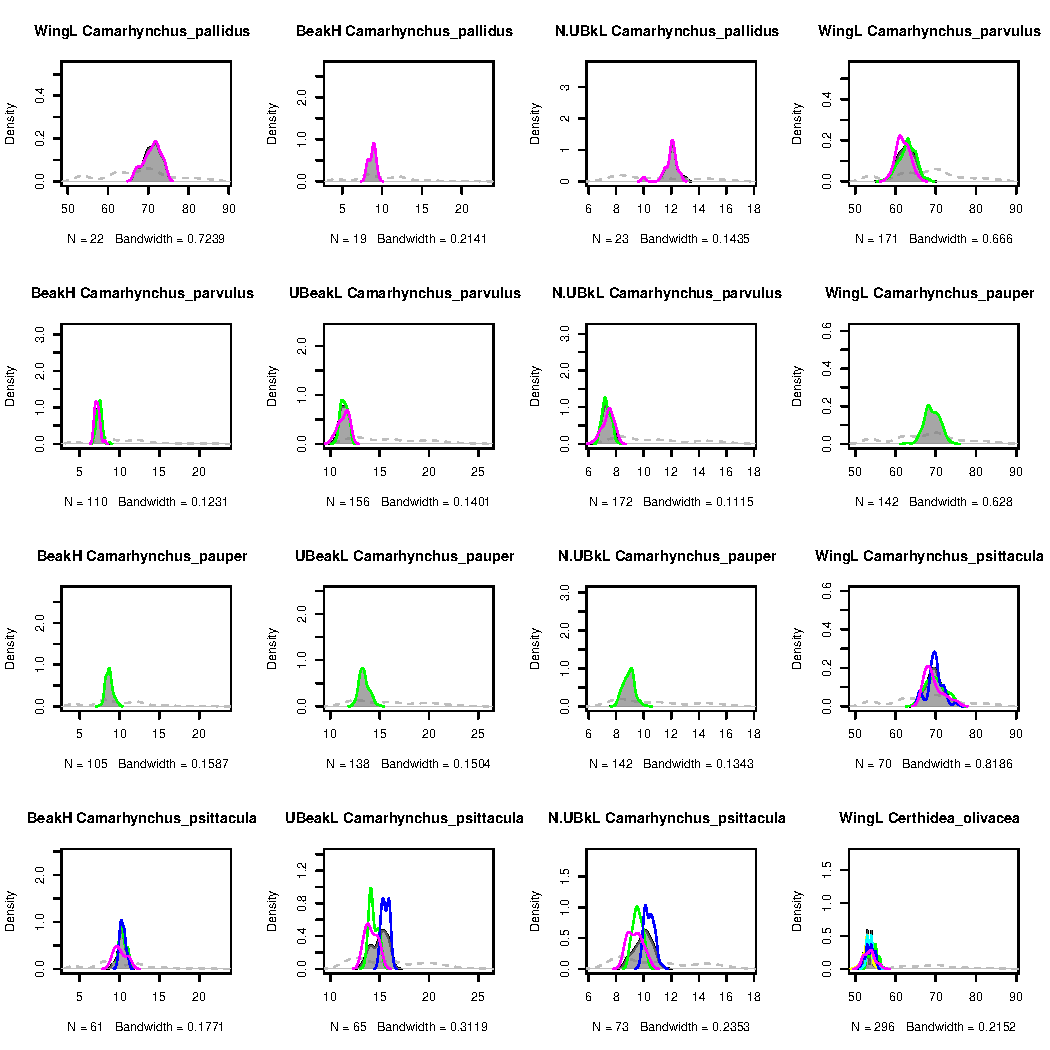
\includegraphics[width=\maxwidth]{figure/unnamed-chunk-41} 

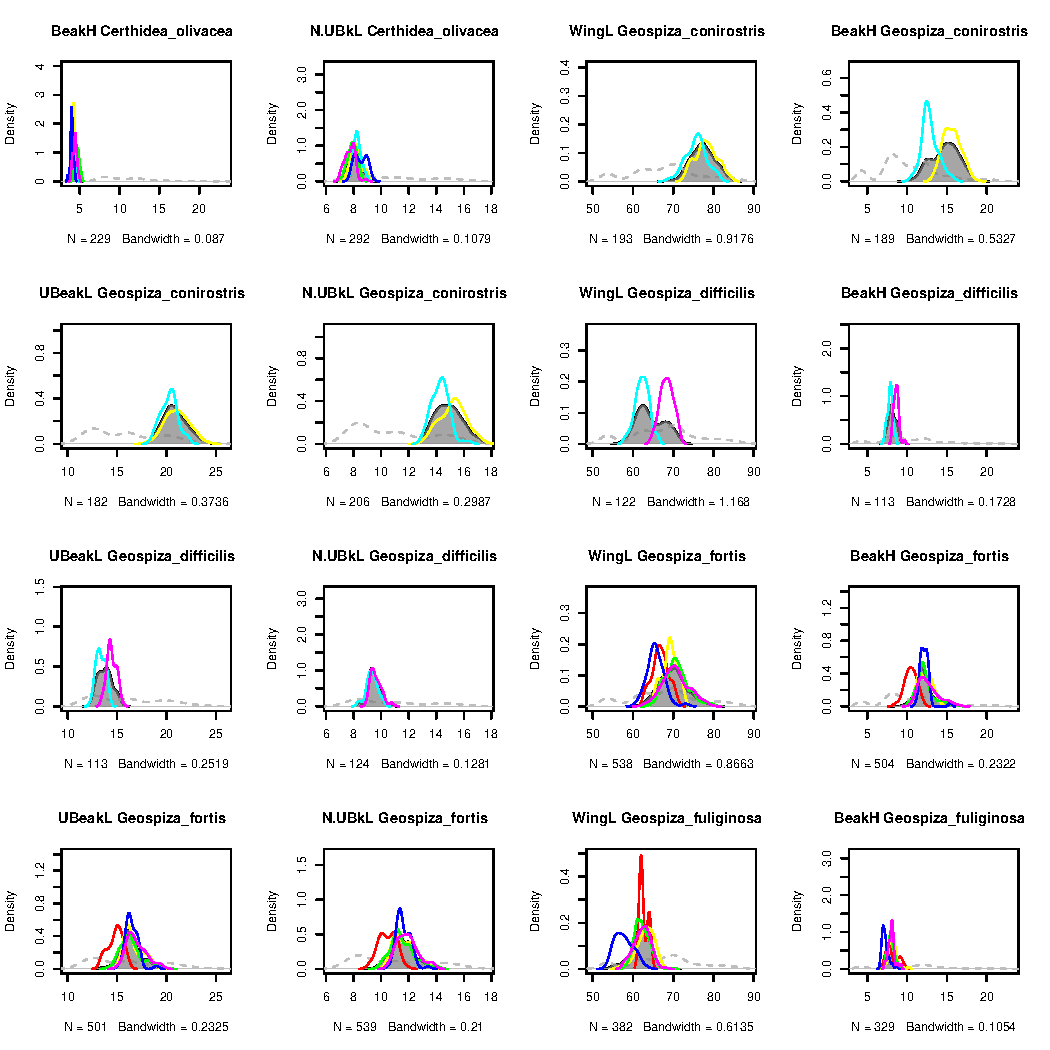
\includegraphics[width=\maxwidth]{figure/unnamed-chunk-42} 

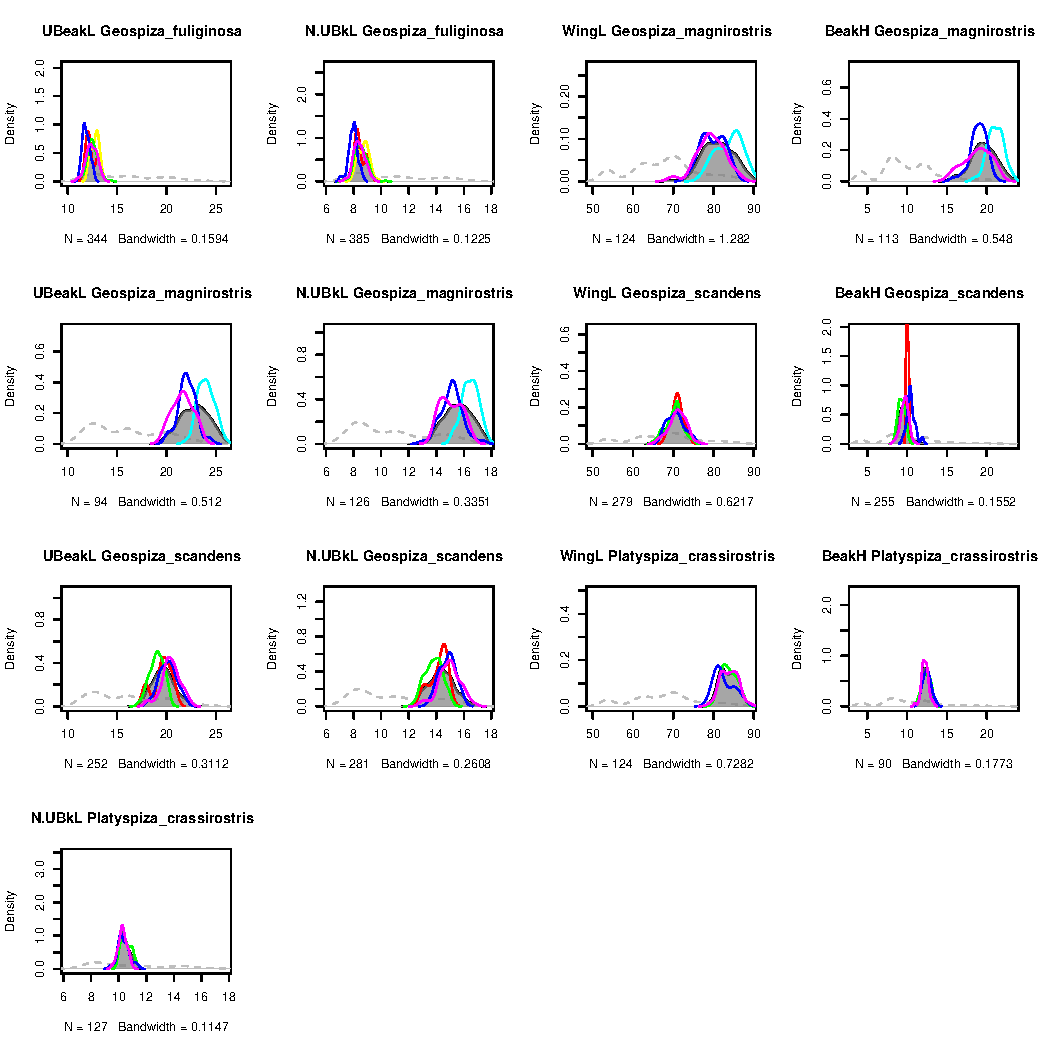
\includegraphics[width=\maxwidth]{figure/unnamed-chunk-43} 

\end{knitrout}


\newpage

Then we can inverse the second and the third arguments to plot the distribution for all finches species. 
\begin{knitrout}
\definecolor{shadecolor}{rgb}{0.969, 0.969, 0.969}\color{fgcolor}\begin{kframe}
\begin{alltt}
\hlkwd{par}\hlstd{(}\hlkwc{mfrow} \hlstd{=} \hlkwd{c}\hlstd{(}\hlnum{5}\hlstd{,} \hlnum{5}\hlstd{),} \hlkwc{cex} \hlstd{=} \hlnum{0.5}\hlstd{)}
\hlkwd{plot_dens}\hlstd{(traits.finch, ind.plot.finch, sp.finch,} \hlkwc{ylim.cex} \hlstd{=} \hlnum{8}\hlstd{,} \hlkwc{plot.ask} \hlstd{= F,}
    \hlkwc{multipanel} \hlstd{= F,} \hlkwc{leg} \hlstd{= F)}
\end{alltt}
\end{kframe}
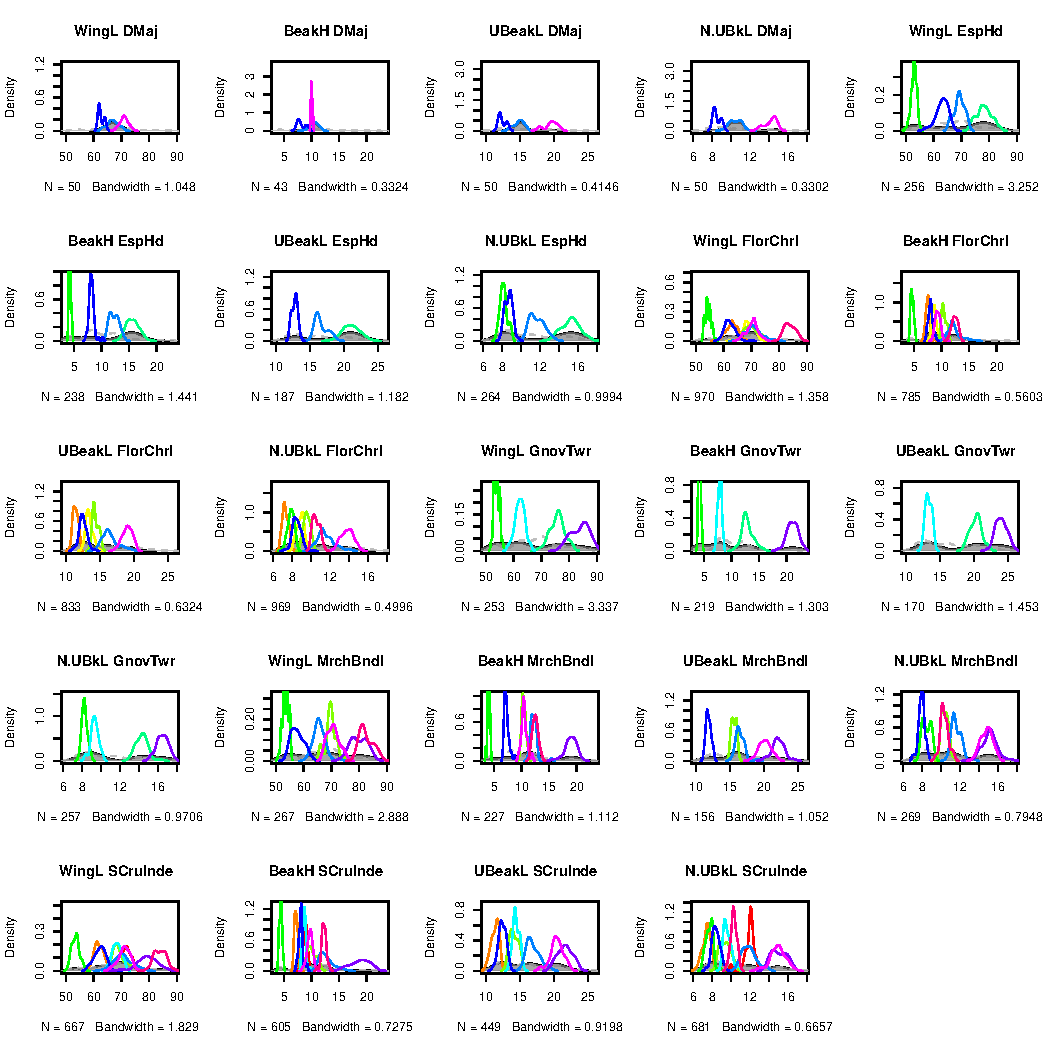
\includegraphics[width=\maxwidth]{figure/unnamed-chunk-5} 

\end{knitrout}


\begin{knitrout}
\definecolor{shadecolor}{rgb}{0.969, 0.969, 0.969}\color{fgcolor}\begin{kframe}
\begin{alltt}
\hlkwd{plot_dens}\hlstd{(traits.finch,} \hlkwd{rep}\hlstd{(}\hlstr{"region"}\hlstd{,} \hlkwc{times} \hlstd{=} \hlkwd{dim}\hlstd{(traits.finch)[}\hlnum{1}\hlstd{]), sp.finch,}
    \hlkwc{ylim.cex} \hlstd{=} \hlnum{6}\hlstd{,} \hlkwc{plot.ask} \hlstd{= F,} \hlkwc{leg} \hlstd{= F)}
\end{alltt}
\end{kframe}
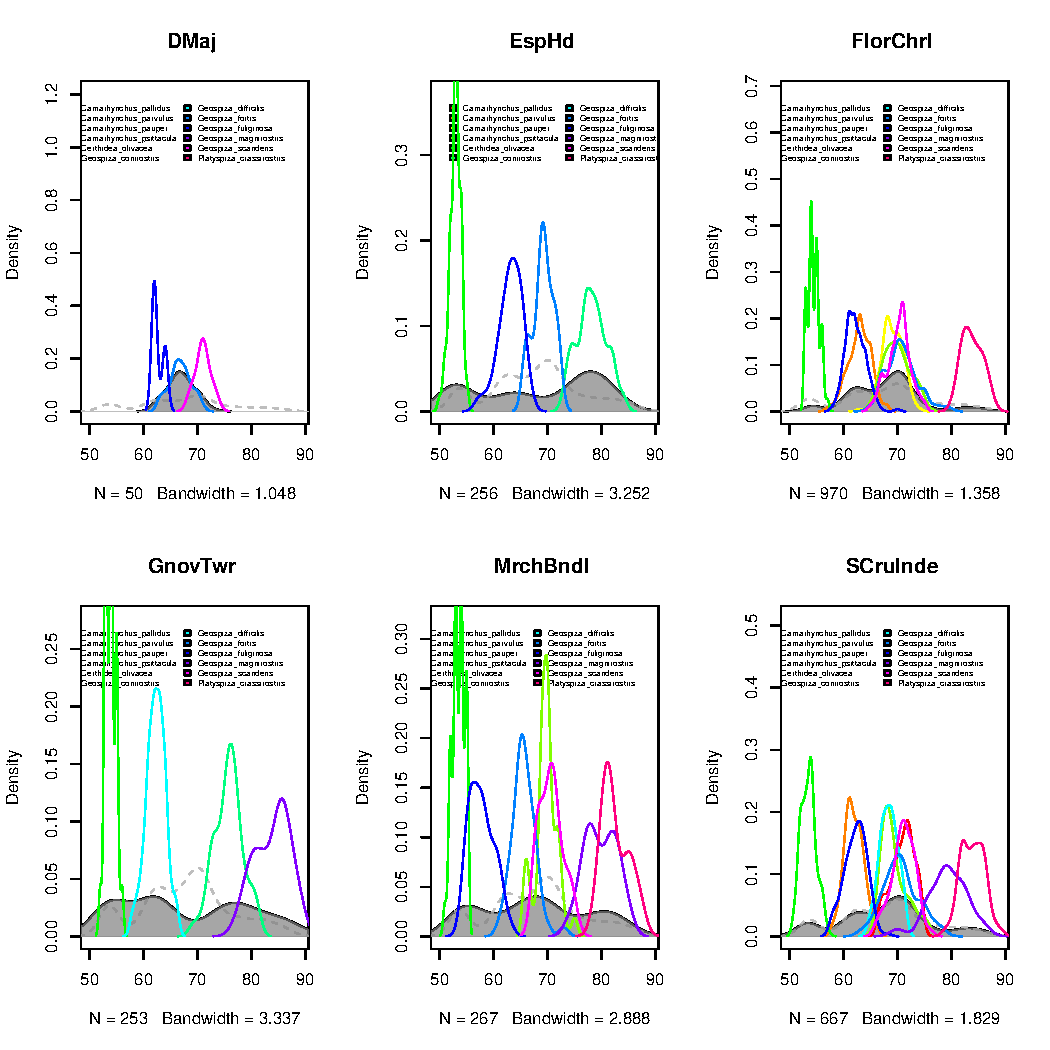
\includegraphics[width=\maxwidth]{figure/unnamed-chunk-6} 

\end{knitrout}


\begin{knitrout}
\definecolor{shadecolor}{rgb}{0.969, 0.969, 0.969}\color{fgcolor}\begin{kframe}
\begin{alltt}
\hlkwd{plot_dens}\hlstd{(traits.finch,} \hlkwd{rep}\hlstd{(}\hlstr{"toutes_sp"}\hlstd{,} \hlkwc{times} \hlstd{=} \hlkwd{dim}\hlstd{(traits.finch)[}\hlnum{1}\hlstd{]), ind.plot.finch,}
    \hlkwc{ylim.cex} \hlstd{=} \hlnum{3}\hlstd{,} \hlkwc{plot.ask} \hlstd{= F)}
\end{alltt}
\end{kframe}
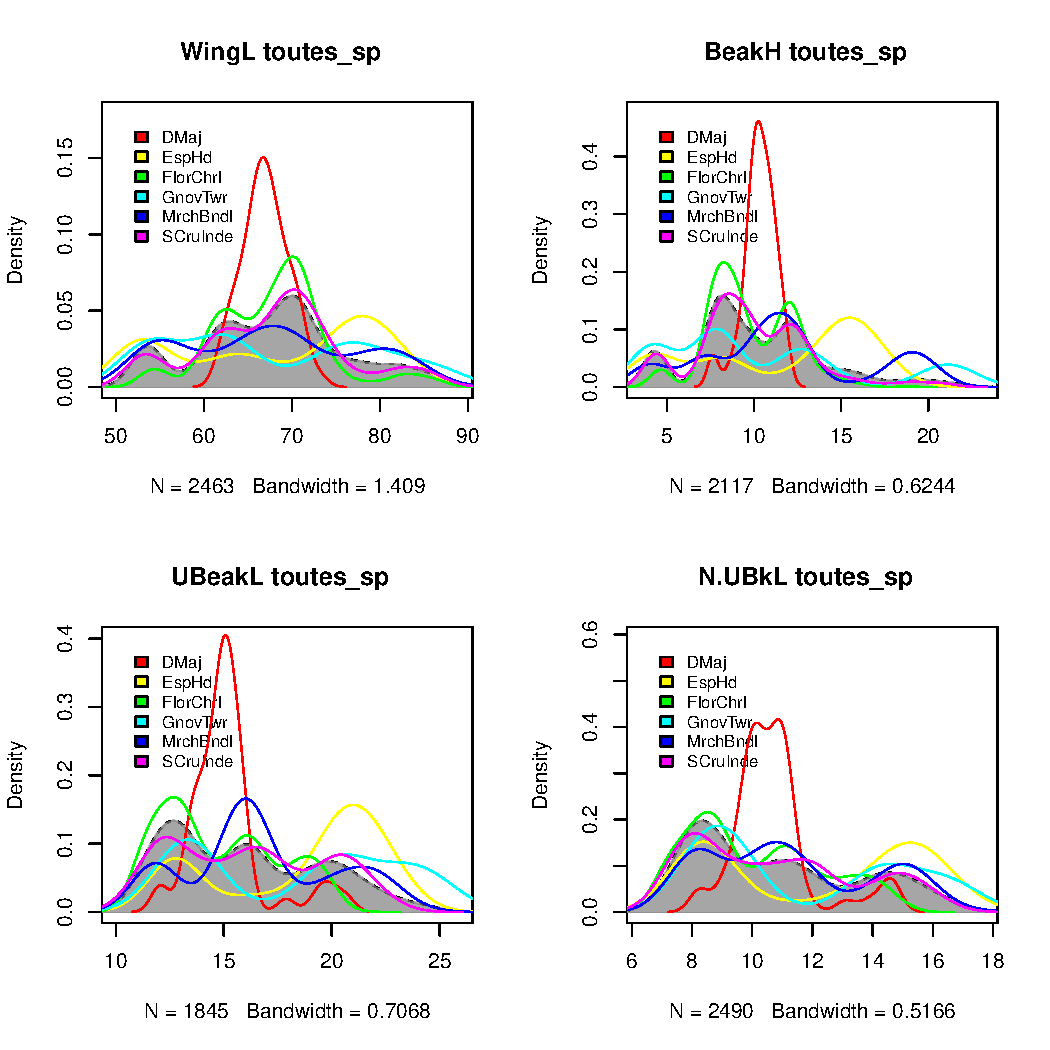
\includegraphics[width=\maxwidth]{figure/unnamed-chunk-7} 

\end{knitrout}




\newpage

%%%%%%%%%%%%%%%%
\section{Decomposition of variances}
%%%%%%%%%%%%%%%%

\subsection{Decomposition of within/among species variances}

\begin{knitrout}
\definecolor{shadecolor}{rgb}{0.969, 0.969, 0.969}\color{fgcolor}\begin{kframe}
\begin{alltt}
\hlstd{comm} \hlkwb{<-} \hlkwd{t}\hlstd{(}\hlkwd{table}\hlstd{(ind.plot.finch,} \hlnum{1}\hlopt{:}\hlkwd{length}\hlstd{(ind.plot.finch)))}
\hlstd{comm.sp} \hlkwb{<-} \hlkwd{table}\hlstd{(sp.finch, ind.plot.finch)}
\hlkwd{class}\hlstd{(comm.sp)} \hlkwb{<-} \hlstr{"matrix"}

\hlstd{traits.finch.sp} \hlkwb{<-} \hlkwd{apply}\hlstd{(}\hlkwd{apply}\hlstd{(traits.finch,} \hlnum{2}\hlstd{, scale),} \hlnum{2}\hlstd{,} \hlkwa{function}\hlstd{(}\hlkwc{x}\hlstd{)} \hlkwd{tapply}\hlstd{(x,}
    \hlstd{sp.finch, mean,} \hlkwc{na.rm} \hlstd{= T))}

\hlstd{mat.dist} \hlkwb{<-} \hlkwd{as.matrix}\hlstd{(}\hlkwd{dist}\hlstd{(traits.finch.sp))}\hlopt{^}\hlnum{2}

\hlstd{res.rao} \hlkwb{<-} \hlkwd{RaoRel}\hlstd{(}\hlkwc{sample} \hlstd{=} \hlkwd{as.matrix}\hlstd{(comm.sp),} \hlkwc{dfunc} \hlstd{= mat.dist,} \hlkwc{dphyl} \hlstd{=} \hlkwa{NULL}\hlstd{,}
    \hlkwc{weight} \hlstd{= F,} \hlkwc{Jost} \hlstd{= F,} \hlkwc{structure} \hlstd{=} \hlkwa{NULL}\hlstd{)}

\hlstd{witRao} \hlkwb{<-} \hlstd{res.rao}\hlopt{$}\hlstd{FD}\hlopt{$}\hlstd{Mean_Alpha}  \hlcom{#overall within species variance}
\hlstd{betRao} \hlkwb{<-} \hlstd{res.rao}\hlopt{$}\hlstd{FD}\hlopt{$}\hlstd{Beta_add}  \hlcom{#between species variance}
\hlstd{totRao} \hlkwb{<-} \hlstd{res.rao}\hlopt{$}\hlstd{FD}\hlopt{$}\hlstd{Gamma}  \hlcom{#the total variance}

\hlstd{witRao} \hlopt{+} \hlstd{betRao}
\end{alltt}
\begin{verbatim}
## [1] 8.37
\end{verbatim}
\begin{alltt}
\hlstd{totRao}
\end{alltt}
\begin{verbatim}
## [1] 8.37
\end{verbatim}
\end{kframe}
\end{knitrout}


Now let's take the abundance to calculate Rao diversity.

\begin{knitrout}
\definecolor{shadecolor}{rgb}{0.969, 0.969, 0.969}\color{fgcolor}\begin{kframe}
\begin{alltt}
\hlstd{res.rao.w} \hlkwb{<-} \hlkwd{RaoRel}\hlstd{(}\hlkwc{sample} \hlstd{=} \hlkwd{as.matrix}\hlstd{(comm.sp),} \hlkwc{dfunc} \hlstd{= mat.dist,} \hlkwc{dphyl} \hlstd{=} \hlkwa{NULL}\hlstd{,}
    \hlkwc{weight} \hlstd{= T,} \hlkwc{Jost} \hlstd{= F,} \hlkwc{structure} \hlstd{=} \hlkwa{NULL}\hlstd{)}

\hlstd{witRao.w} \hlkwb{<-} \hlstd{res.rao.w}\hlopt{$}\hlstd{FD}\hlopt{$}\hlstd{Mean_Alpha}  \hlcom{#overall within species variance}
\hlstd{betRao.w} \hlkwb{<-} \hlstd{res.rao.w}\hlopt{$}\hlstd{FD}\hlopt{$}\hlstd{Beta_add}  \hlcom{#between species variance}
\hlstd{totRao.w} \hlkwb{<-} \hlstd{res.rao.w}\hlopt{$}\hlstd{FD}\hlopt{$}\hlstd{Gamma}  \hlcom{#the total variance}

\hlstd{witRao.w}
\end{alltt}
\begin{verbatim}
## [1] 7.551
\end{verbatim}
\begin{alltt}
\hlstd{betRao.w}
\end{alltt}
\begin{verbatim}
## [1] 0.3458
\end{verbatim}
\end{kframe}
\end{knitrout}


Plot the results

\begin{knitrout}
\definecolor{shadecolor}{rgb}{0.969, 0.969, 0.969}\color{fgcolor}\begin{kframe}
\begin{alltt}
\hlkwd{barplot}\hlstd{(}\hlkwd{cbind}\hlstd{(}\hlkwd{c}\hlstd{(witRao.w, betRao.w),} \hlkwd{c}\hlstd{(witRao, betRao)),} \hlkwc{names.arg} \hlstd{=} \hlkwd{c}\hlstd{(}\hlstr{"abundance"}\hlstd{,}
    \hlstr{"presence"}\hlstd{),} \hlkwc{legend.text} \hlstd{=} \hlkwd{c}\hlstd{(}\hlstr{"within species"}\hlstd{,} \hlstr{"between species"}\hlstd{),} \hlkwc{ylab} \hlstd{=} \hlstr{"Rao"}\hlstd{,}
    \hlkwc{ylim} \hlstd{=} \hlkwd{c}\hlstd{(}\hlnum{0}\hlstd{,} \hlnum{10}\hlstd{))}
\end{alltt}
\end{kframe}

{\centering 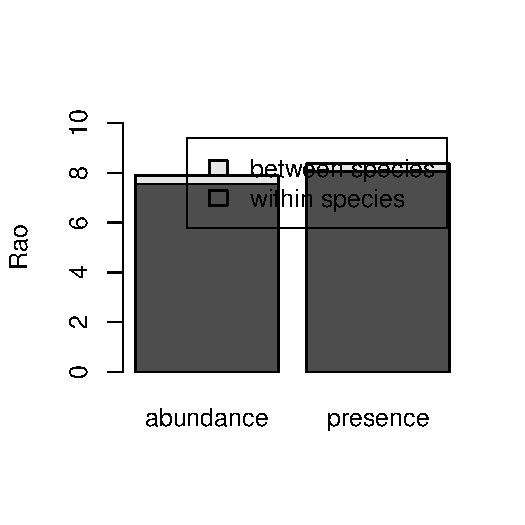
\includegraphics[width=\maxwidth]{figure/unnamed-chunk-10} 

}



\end{knitrout}


We can do this analysis for each trait separately. We need to replace (or exclude) NA values. For this example, we use the package mice to complete the data.

\begin{knitrout}
\definecolor{shadecolor}{rgb}{0.969, 0.969, 0.969}\color{fgcolor}\begin{kframe}
\begin{alltt}
\hlstd{comm} \hlkwb{<-} \hlkwd{t}\hlstd{(}\hlkwd{table}\hlstd{(ind.plot.finch,} \hlnum{1}\hlopt{:}\hlkwd{length}\hlstd{(ind.plot.finch)))}

\hlkwd{require}\hlstd{(mice)}
\hlstd{traits} \hlkwb{=} \hlstd{traits.finch}
\hlstd{mice} \hlkwb{<-} \hlkwd{mice}\hlstd{(traits.finch)}
\hlstd{traits.finch.mice} \hlkwb{<-} \hlkwd{complete}\hlstd{(mice)}
\end{alltt}
\end{kframe}
\end{knitrout}



\begin{knitrout}
\definecolor{shadecolor}{rgb}{0.969, 0.969, 0.969}\color{fgcolor}\begin{kframe}
\begin{alltt}
\hlstd{traits.finch.mice.sp} \hlkwb{<-} \hlkwd{apply}\hlstd{(}\hlkwd{apply}\hlstd{(traits.finch.mice,} \hlnum{2}\hlstd{, scale),} \hlnum{2}\hlstd{,} \hlkwa{function}\hlstd{(}\hlkwc{x}\hlstd{)} \hlkwd{tapply}\hlstd{(x,}
    \hlstd{sp.finch, mean,} \hlkwc{na.rm} \hlstd{= T))}

\hlstd{trait.rao.w} \hlkwb{<-} \hlkwd{list}\hlstd{()}
\hlstd{witRao.w.bytrait} \hlkwb{<-} \hlkwd{c}\hlstd{()}
\hlstd{betRao.w.bytrait} \hlkwb{<-} \hlkwd{c}\hlstd{()}
\hlkwa{for} \hlstd{(t} \hlkwa{in} \hlnum{1}\hlopt{:}\hlnum{4}\hlstd{) \{}
    \hlstd{trait.rao.w[[t]]} \hlkwb{<-} \hlkwd{RaoRel}\hlstd{(}\hlkwc{sample} \hlstd{=} \hlkwd{as.matrix}\hlstd{(comm.sp),} \hlkwc{dfunc} \hlstd{=} \hlkwd{dist}\hlstd{(traits.finch.mice.sp[,}
        \hlstd{t]),} \hlkwc{dphyl} \hlstd{=} \hlkwa{NULL}\hlstd{,} \hlkwc{weight} \hlstd{= T,} \hlkwc{Jost} \hlstd{= F,} \hlkwc{structure} \hlstd{=} \hlkwa{NULL}\hlstd{)}
    \hlstd{witRao.w.bytrait} \hlkwb{<-} \hlkwd{c}\hlstd{(witRao.w.bytrait, trait.rao.w[[t]]}\hlopt{$}\hlstd{FD}\hlopt{$}\hlstd{Mean_Alpha)}
    \hlstd{betRao.w.bytrait} \hlkwb{<-} \hlkwd{c}\hlstd{(betRao.w.bytrait, trait.rao.w[[t]]}\hlopt{$}\hlstd{FD}\hlopt{$}\hlstd{Beta_add)}
\hlstd{\}}
\end{alltt}
\end{kframe}
\end{knitrout}



Plot the results by traits.

\begin{knitrout}
\definecolor{shadecolor}{rgb}{0.969, 0.969, 0.969}\color{fgcolor}\begin{kframe}
\begin{alltt}
\hlkwd{barplot}\hlstd{(}\hlkwd{t}\hlstd{(}\hlkwd{cbind}\hlstd{(witRao.w.bytrait, betRao.w.bytrait)),} \hlkwc{names.arg} \hlstd{=} \hlkwd{colnames}\hlstd{(traits.finch),}
    \hlkwc{legend.text} \hlstd{=} \hlkwd{c}\hlstd{(}\hlstr{"within species"}\hlstd{,} \hlstr{"between species"}\hlstd{),} \hlkwc{ylab} \hlstd{=} \hlstr{"Rao"}\hlstd{,} \hlkwc{ylim} \hlstd{=} \hlkwd{c}\hlstd{(}\hlnum{0}\hlstd{,}
        \hlnum{1.5}\hlstd{))}
\end{alltt}
\end{kframe}
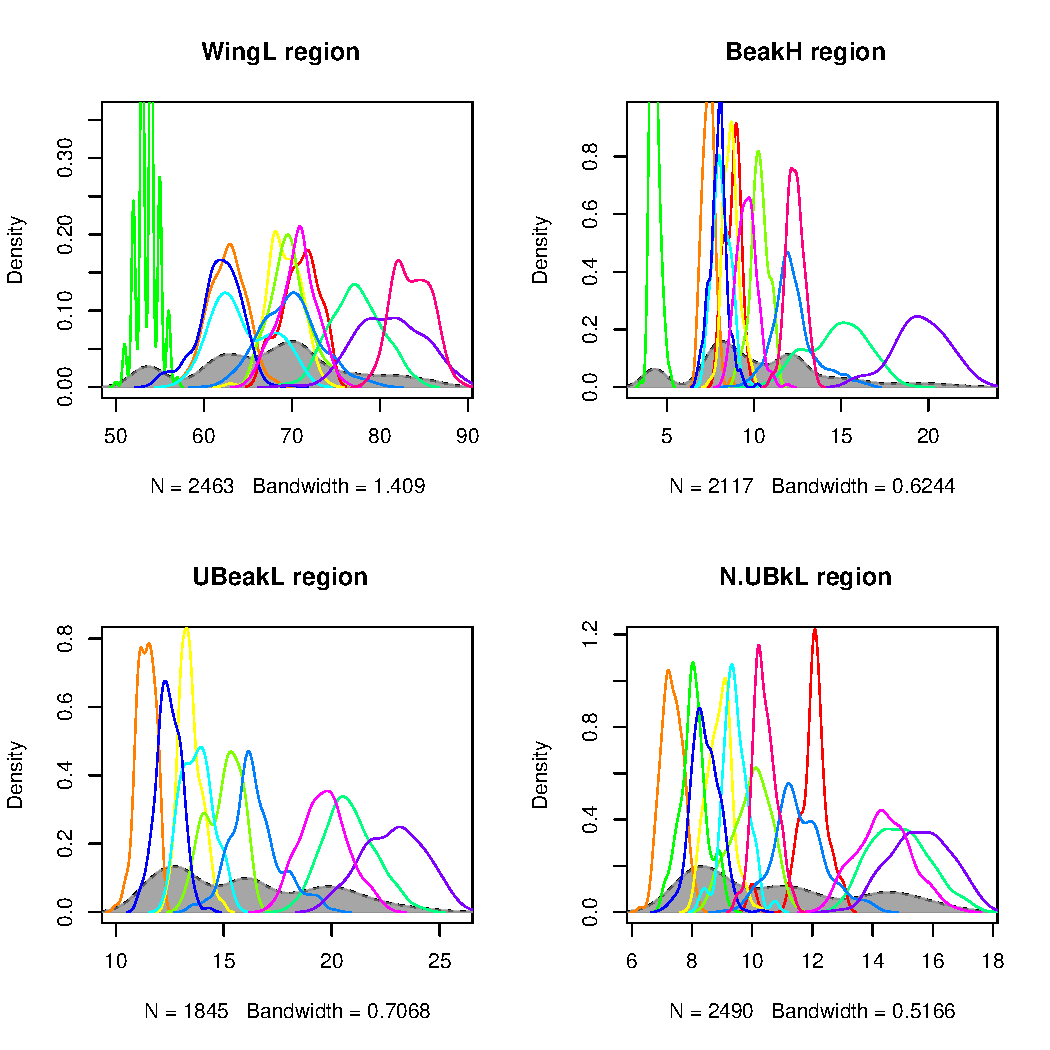
\includegraphics[width=\maxwidth]{figure/unnamed-chunk-13} 

\end{knitrout}



\subsection{Decomposition of within/among species variances}

\begin{knitrout}
\definecolor{shadecolor}{rgb}{0.969, 0.969, 0.969}\color{fgcolor}\begin{kframe}
\begin{alltt}
\hlstd{res.decomp} \hlkwb{<-} \hlkwd{decomp_within}\hlstd{(}\hlkwc{traits} \hlstd{= traits.finch,} \hlkwc{sp} \hlstd{= sp.finch,} \hlkwc{ind.plot} \hlstd{= ind.plot.finch,}
    \hlkwc{print} \hlstd{=} \hlnum{FALSE}\hlstd{)}

\hlkwd{barplot.decomp_within}\hlstd{(res.decomp)}
\end{alltt}
\end{kframe}

{\centering 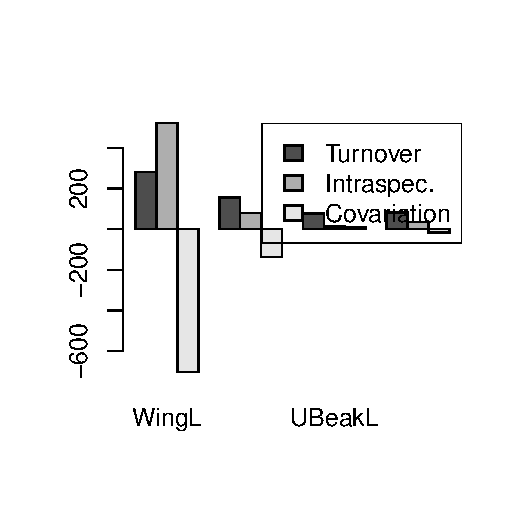
\includegraphics[width=\maxwidth]{figure/unnamed-chunk-141} 

}


\begin{kframe}\begin{alltt}
\hlkwd{par}\hlstd{(}\hlkwc{mfrow} \hlstd{=} \hlkwd{c}\hlstd{(}\hlnum{2}\hlstd{,} \hlnum{2}\hlstd{))}
\hlkwd{barplot.decomp_within}\hlstd{(res.decomp,} \hlkwc{resume} \hlstd{= F)}
\end{alltt}
\end{kframe}

{\centering 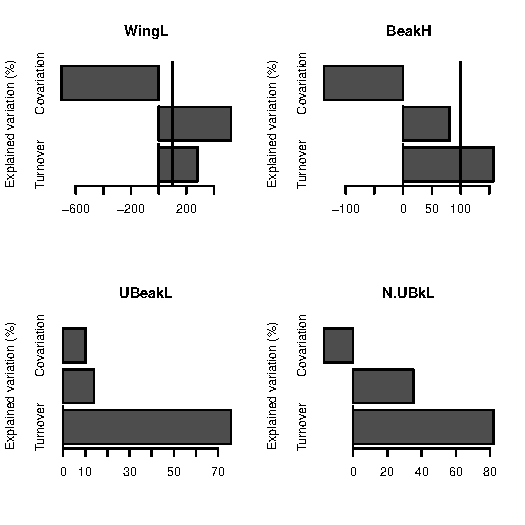
\includegraphics[width=\maxwidth]{figure/unnamed-chunk-142} 

}


\begin{kframe}\begin{alltt}
\hlkwd{par}\hlstd{(}\hlkwc{mfrow} \hlstd{=} \hlkwd{c}\hlstd{(}\hlnum{1}\hlstd{,} \hlnum{1}\hlstd{))}
\end{alltt}
\end{kframe}
\end{knitrout}



\newpage

\subsection{Decomposition of variances using nested factors}

\begin{knitrout}
\definecolor{shadecolor}{rgb}{0.969, 0.969, 0.969}\color{fgcolor}\begin{kframe}
\begin{alltt}
\hlstd{vec} \hlkwb{<-} \hlkwd{seq}\hlstd{(}\hlnum{1}\hlstd{,} \hlkwd{length}\hlstd{(sp.finch)} \hlopt{*} \hlnum{2}\hlstd{,} \hlkwc{by} \hlstd{=} \hlnum{2}\hlstd{)}
\hlstd{genus} \hlkwb{<-} \hlkwd{as.vector}\hlstd{(}\hlkwd{unlist}\hlstd{(}\hlkwd{strsplit}\hlstd{(}\hlkwd{as.vector}\hlstd{(sp.finch),} \hlstr{"_"}\hlstd{))[vec])}
\hlstd{fact} \hlkwb{<-} \hlkwd{cbind}\hlstd{(}\hlkwc{genus} \hlstd{=} \hlkwd{as.factor}\hlstd{(genus),} \hlkwc{species} \hlstd{=} \hlkwd{as.factor}\hlstd{(}\hlkwd{as.vector}\hlstd{(sp.finch)),}
    \hlkwc{sites} \hlstd{=} \hlkwd{as.factor}\hlstd{(}\hlkwd{as.vector}\hlstd{(ind.plot.finch)))}

\hlstd{res.partvar.finch} \hlkwb{<-} \hlkwd{partvar}\hlstd{(}\hlkwc{traits} \hlstd{= traits.finch,} \hlkwc{factors} \hlstd{= fact)}

\hlstd{res.partvar.finch}
\end{alltt}
\end{kframe}
\end{knitrout}



\begin{knitrout}
\definecolor{shadecolor}{rgb}{0.969, 0.969, 0.969}\color{fgcolor}\begin{kframe}
\begin{alltt}
\hlkwd{par}\hlstd{(}\hlkwc{mfrow} \hlstd{=} \hlkwd{c}\hlstd{(}\hlnum{2}\hlstd{,} \hlnum{2}\hlstd{),} \hlkwc{mai} \hlstd{=} \hlkwd{c}\hlstd{(}\hlnum{0.2}\hlstd{,} \hlnum{0.2}\hlstd{,} \hlnum{0.2}\hlstd{,} \hlnum{0.2}\hlstd{))}
\hlstd{colors} \hlkwb{<-} \hlkwd{c}\hlstd{(}\hlkwd{rgb}\hlstd{(}\hlnum{102}\hlstd{,} \hlnum{167}\hlstd{,} \hlnum{0}\hlstd{,} \hlkwc{maxColorValue} \hlstd{=} \hlnum{255}\hlstd{),} \hlkwd{rgb}\hlstd{(}\hlnum{185}\hlstd{,} \hlnum{210}\hlstd{,} \hlnum{0}\hlstd{,} \hlkwc{maxColorValue} \hlstd{=} \hlnum{255}\hlstd{),}
    \hlkwd{rgb}\hlstd{(}\hlnum{98}\hlstd{,} \hlnum{174}\hlstd{,} \hlnum{255}\hlstd{,} \hlkwc{maxColorValue} \hlstd{=} \hlnum{255}\hlstd{),} \hlkwd{rgb}\hlstd{(}\hlnum{158}\hlstd{,} \hlnum{30}\hlstd{,} \hlnum{240}\hlstd{,} \hlkwc{maxColorValue} \hlstd{=} \hlnum{255}\hlstd{))}

\hlkwd{pie_partvar}\hlstd{(res.partvar.finch,} \hlkwc{col} \hlstd{= colors)}
\end{alltt}
\end{kframe}

{\centering 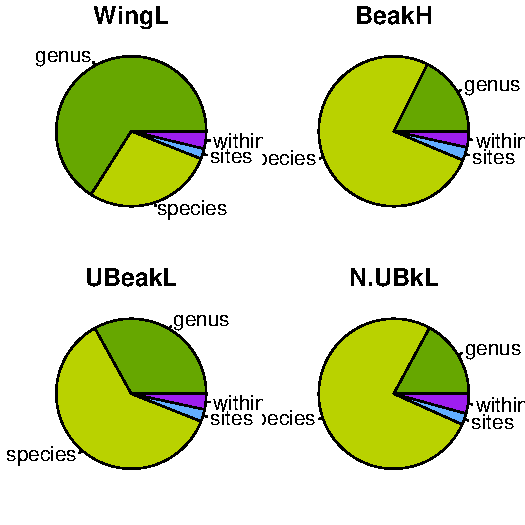
\includegraphics[width=\maxwidth]{figure/unnamed-chunk-161} 

}


\begin{kframe}\begin{alltt}
\hlkwd{par}\hlstd{(oldpar)}

\hlkwd{bar_partvar}\hlstd{(res.partvar.finch,} \hlkwc{col} \hlstd{= colors,} \hlkwc{leg} \hlstd{=} \hlnum{TRUE}\hlstd{)}
\end{alltt}
\end{kframe}

{\centering 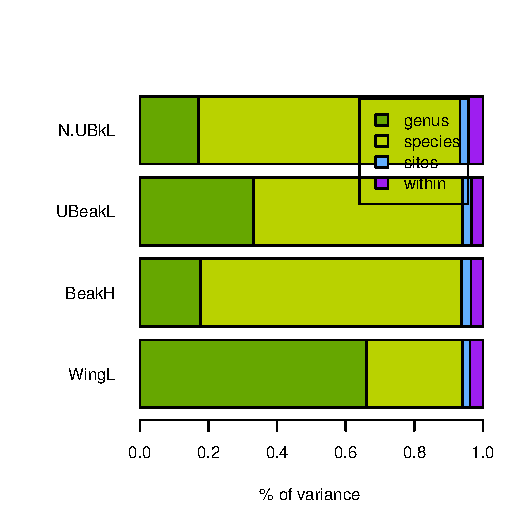
\includegraphics[width=\maxwidth]{figure/unnamed-chunk-162} 

}



\end{knitrout}




\newpage

\subsection{Plot the relation between populational trait means and sites traits means.}

\begin{knitrout}
\definecolor{shadecolor}{rgb}{0.969, 0.969, 0.969}\color{fgcolor}\begin{kframe}
\begin{alltt}
\hlkwd{plot_sp_pop}\hlstd{(traits.finch, ind.plot.finch, sp.finch,} \hlkwc{silent} \hlstd{=} \hlnum{TRUE}\hlstd{)}
\end{alltt}
\end{kframe}
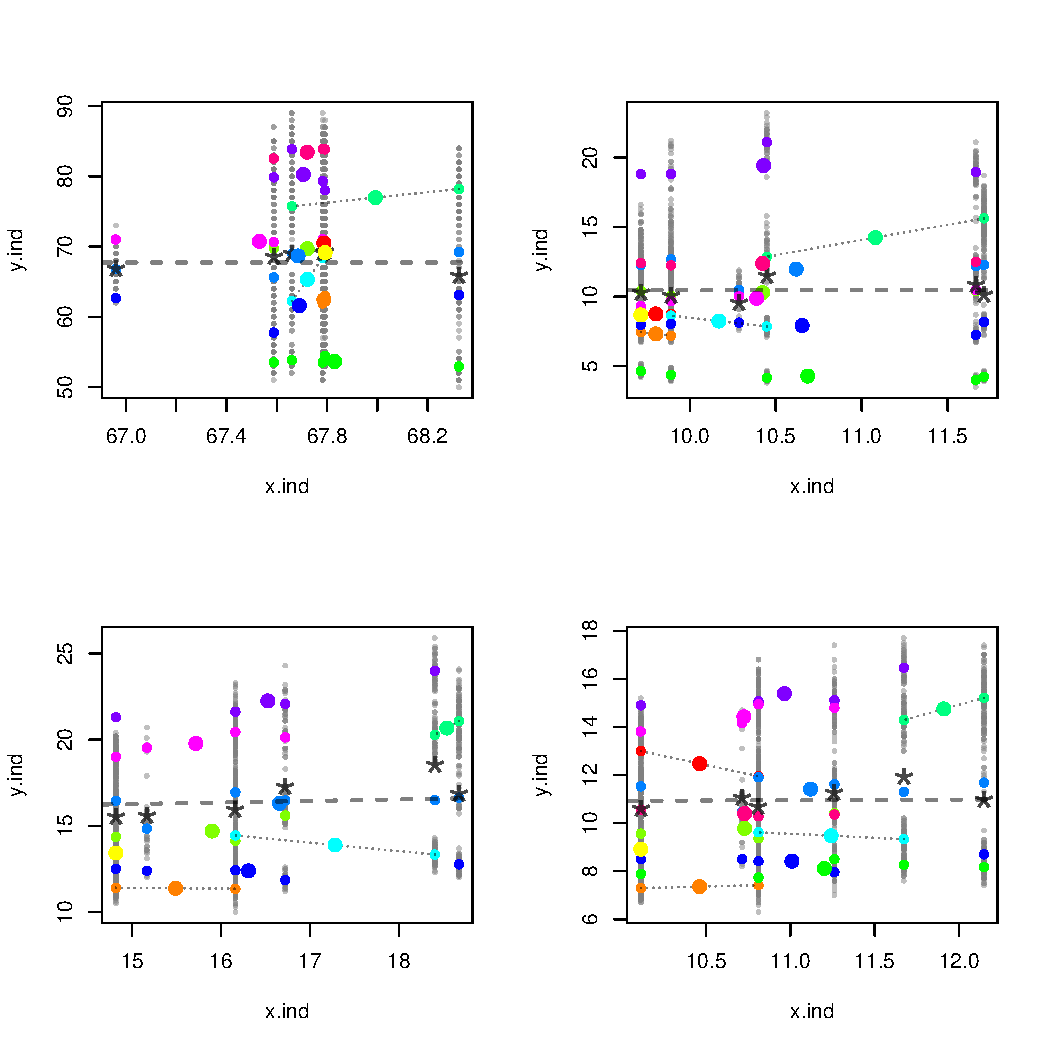
\includegraphics[width=\maxwidth]{figure/unnamed-chunk-17} 

\end{knitrout}


If we change the value of the threshold (alpha=10\% instead of 5\% and the minimum individual to represent singificativity fixed to 3 instead of 10 by default) we can see some significant relationships.

\newpage

\begin{knitrout}
\definecolor{shadecolor}{rgb}{0.969, 0.969, 0.969}\color{fgcolor}\begin{kframe}
\begin{alltt}
\hlkwd{plot_sp_pop}\hlstd{(traits.finch, ind.plot.finch, sp.finch,} \hlkwc{p.val} \hlstd{=} \hlnum{0.1}\hlstd{,} \hlkwc{min.ind.signif} \hlstd{=} \hlnum{3}\hlstd{,}
    \hlkwc{silent} \hlstd{=} \hlnum{TRUE}\hlstd{)}
\end{alltt}
\end{kframe}
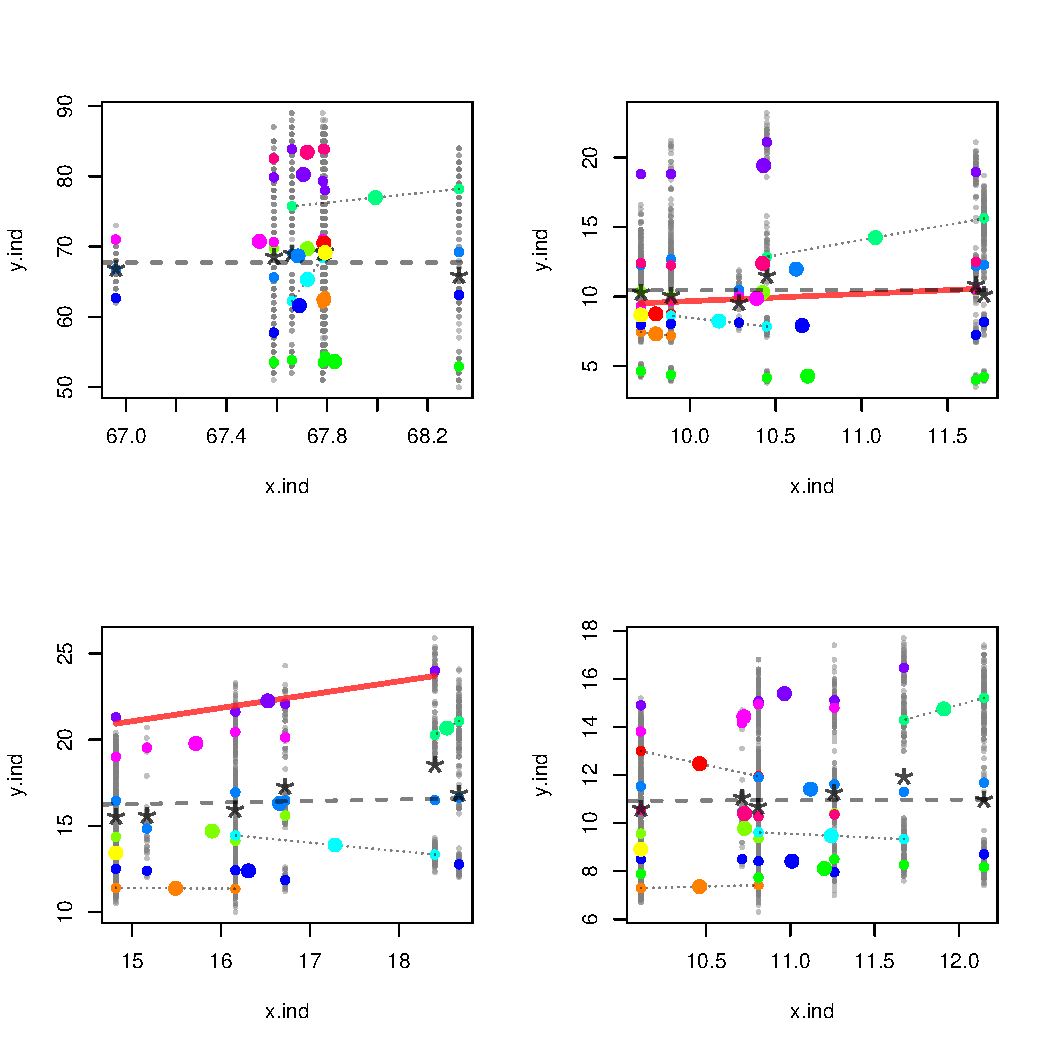
\includegraphics[width=\maxwidth]{figure/unnamed-chunk-18} 

\end{knitrout}


\newpage

For a more simple figure, add the option resume=TRUE. Again if we change the value of the threshold (alpha=10\% instead of 5\% and the minimum individual to represent singificativity fixed to 3 instead of 10 by default) we can see some significant relationships.

\begin{knitrout}
\definecolor{shadecolor}{rgb}{0.969, 0.969, 0.969}\color{fgcolor}\begin{kframe}
\begin{alltt}
\hlkwd{plot_sp_pop}\hlstd{(traits.finch, ind.plot.finch, sp.finch,} \hlkwc{silent} \hlstd{=} \hlnum{TRUE}\hlstd{,} \hlkwc{resume} \hlstd{=} \hlnum{TRUE}\hlstd{,}
    \hlkwc{col.pop} \hlstd{=} \hlstr{"grey"}\hlstd{)}
\end{alltt}
\end{kframe}
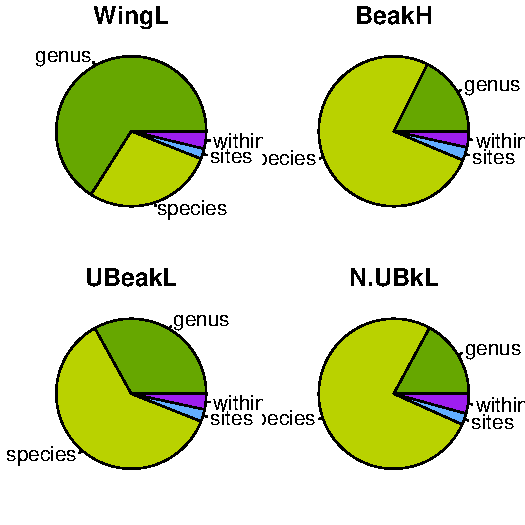
\includegraphics[width=\maxwidth]{figure/unnamed-chunk-191} 
\begin{kframe}\begin{alltt}
\hlkwd{plot_sp_pop}\hlstd{(traits.finch, ind.plot.finch, sp.finch,} \hlkwc{silent} \hlstd{=} \hlnum{TRUE}\hlstd{,} \hlkwc{resume} \hlstd{=} \hlnum{TRUE}\hlstd{,}
    \hlkwc{col.pop} \hlstd{=} \hlstr{"grey"}\hlstd{,} \hlkwc{col.sp} \hlstd{=} \hlstr{"black"}\hlstd{)}
\end{alltt}
\end{kframe}
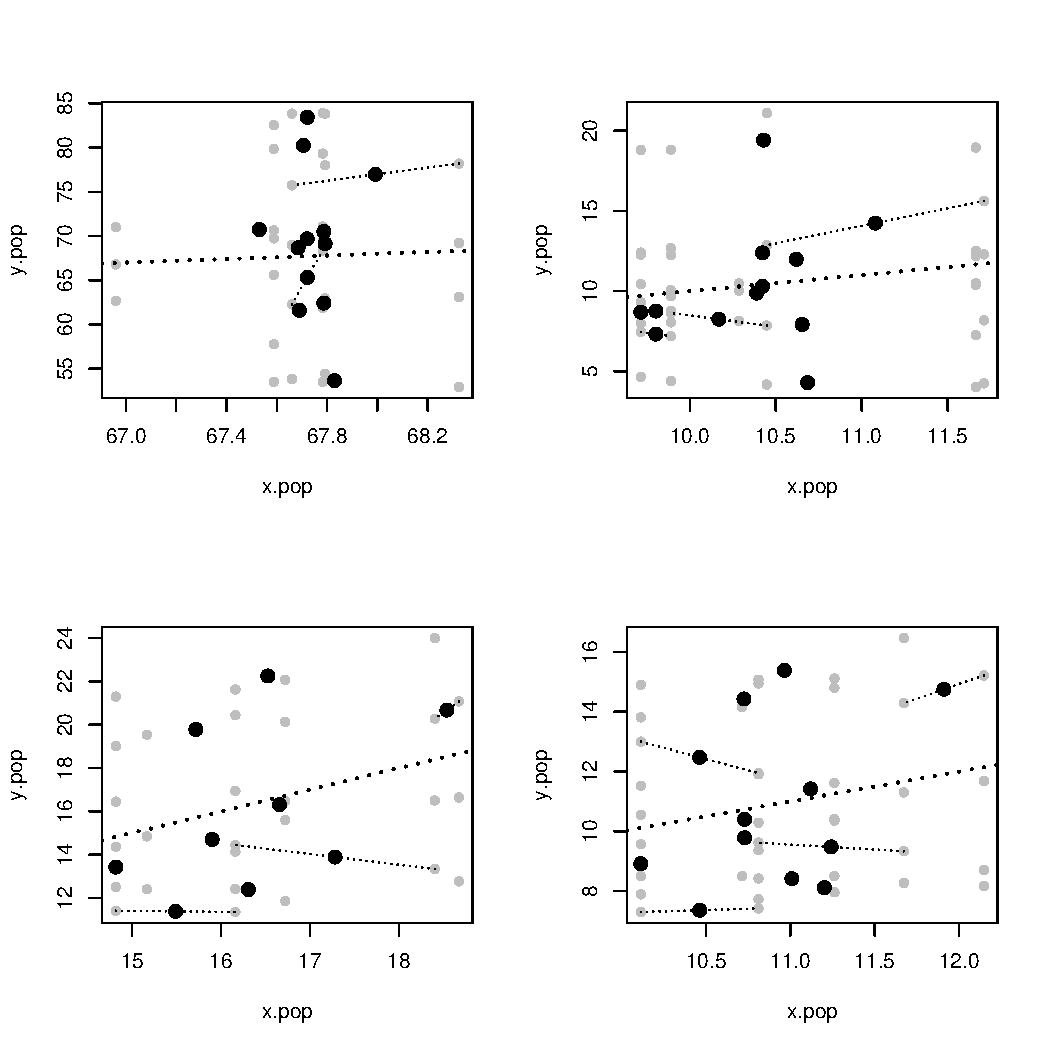
\includegraphics[width=\maxwidth]{figure/unnamed-chunk-192} 
\begin{kframe}\begin{alltt}
\hlkwd{plot_sp_pop}\hlstd{(traits.finch, ind.plot.finch, sp.finch,} \hlkwc{silent} \hlstd{=} \hlnum{TRUE}\hlstd{,} \hlkwc{resume} \hlstd{=} \hlnum{TRUE}\hlstd{,}
    \hlkwc{col.pop} \hlstd{=} \hlstr{"grey"}\hlstd{,} \hlkwc{col.sp} \hlstd{=} \hlstr{"black"}\hlstd{,} \hlkwc{p.val} \hlstd{=} \hlnum{0.1}\hlstd{,} \hlkwc{min.ind.signif} \hlstd{=} \hlnum{3}\hlstd{)}
\end{alltt}
\end{kframe}
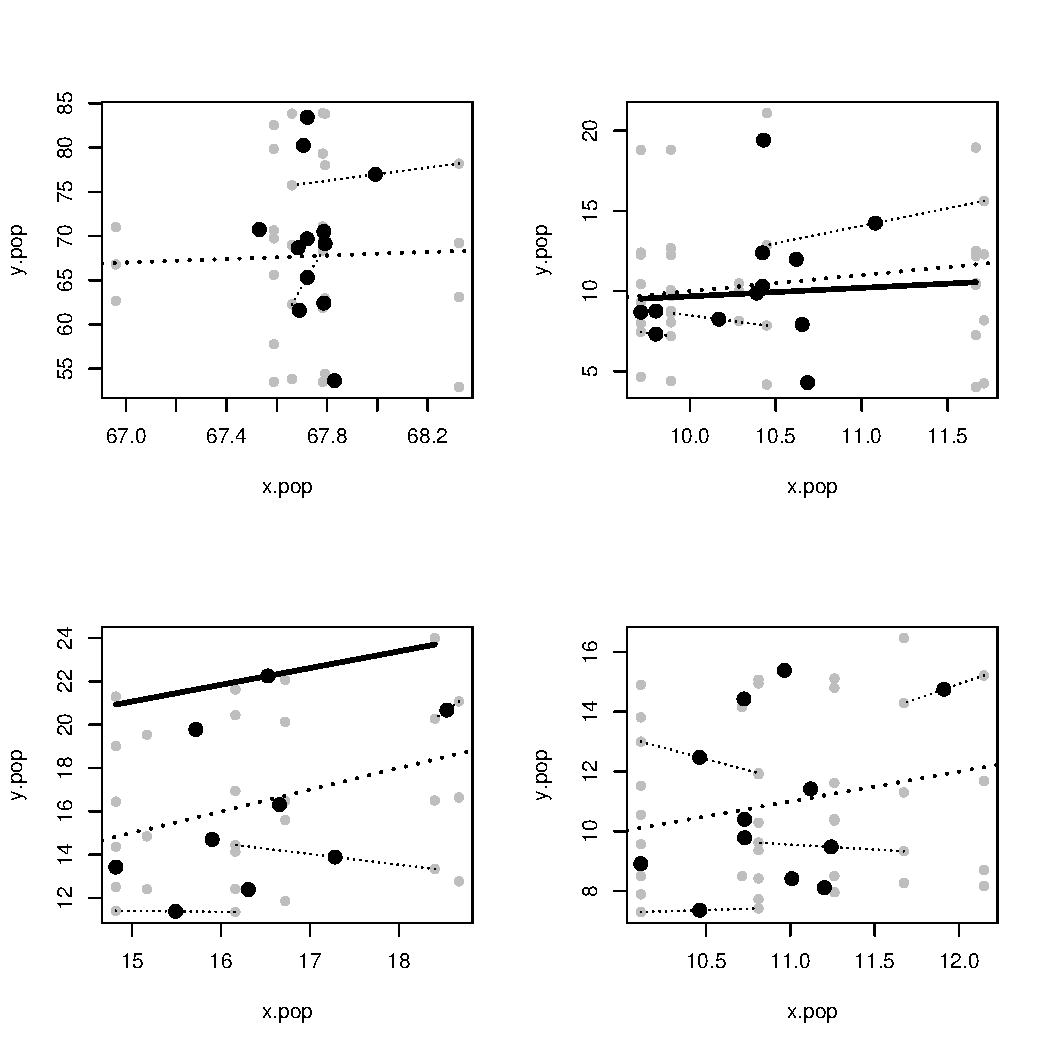
\includegraphics[width=\maxwidth]{figure/unnamed-chunk-193} 

\end{knitrout}




\newpage

%%%%%%%%%%%%%%%%
\section{Test of community assembly}
%%%%%%%%%%%%%%%%

\subsection{Ratio of variances: T-statistics}

\begin{knitrout}
\definecolor{shadecolor}{rgb}{0.969, 0.969, 0.969}\color{fgcolor}\begin{kframe}
\begin{alltt}
\hlstd{res.finch} \hlkwb{<-} \hlkwd{Tstats}\hlstd{(traits.finch,} \hlkwc{ind_plot} \hlstd{= ind.plot.finch,} \hlkwc{sp} \hlstd{= sp.finch,}
    \hlkwc{nperm} \hlstd{=} \hlnum{9}\hlstd{,} \hlkwc{print} \hlstd{=} \hlnum{FALSE}\hlstd{)}
\hlkwd{attributes}\hlstd{(res.finch)}
\end{alltt}
\begin{verbatim}
## $names
## [1] "T_IP.IC"    "T_IC.IR"    "T_PC.PR"    "variances"  "T_IP.IC_nm"
## [6] "T_IC.IR_nm" "T_PC.PR_nm" "pval"      
## 
## $class
## [1] "Tstats"
\end{verbatim}
\end{kframe}
\end{knitrout}


Tstats class is associated to S3 methods plot, barplot and summary

\begin{knitrout}
\definecolor{shadecolor}{rgb}{0.969, 0.969, 0.969}\color{fgcolor}\begin{kframe}
\begin{alltt}
\hlkwd{plot}\hlstd{(res.finch)}
\end{alltt}
\end{kframe}

{\centering 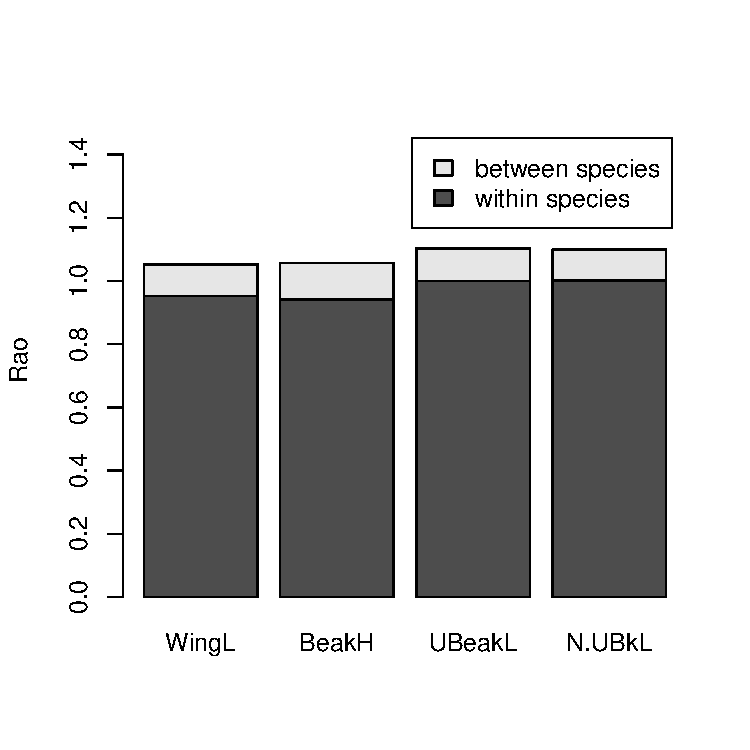
\includegraphics[width=\maxwidth]{figure/unnamed-chunk-21} 

}



\end{knitrout}

\begin{knitrout}
\definecolor{shadecolor}{rgb}{0.969, 0.969, 0.969}\color{fgcolor}\begin{kframe}
\begin{alltt}
\hlkwd{par}\hlstd{(}\hlkwc{mfrow} \hlstd{=} \hlkwd{c}\hlstd{(}\hlnum{2}\hlstd{,} \hlnum{2}\hlstd{))}
\hlkwd{plot}\hlstd{(res.finch,} \hlkwc{type} \hlstd{=} \hlstr{"color_cond"}\hlstd{)}
\hlkwd{plot}\hlstd{(res.finch,} \hlkwc{type} \hlstd{=} \hlstr{"simple"}\hlstd{)}
\hlkwd{plot}\hlstd{(res.finch,} \hlkwc{type} \hlstd{=} \hlstr{"simple_sd"}\hlstd{)}
\hlkwd{plot}\hlstd{(res.finch,} \hlkwc{type} \hlstd{=} \hlstr{"barplot"}\hlstd{)}
\end{alltt}
\end{kframe}

{\centering 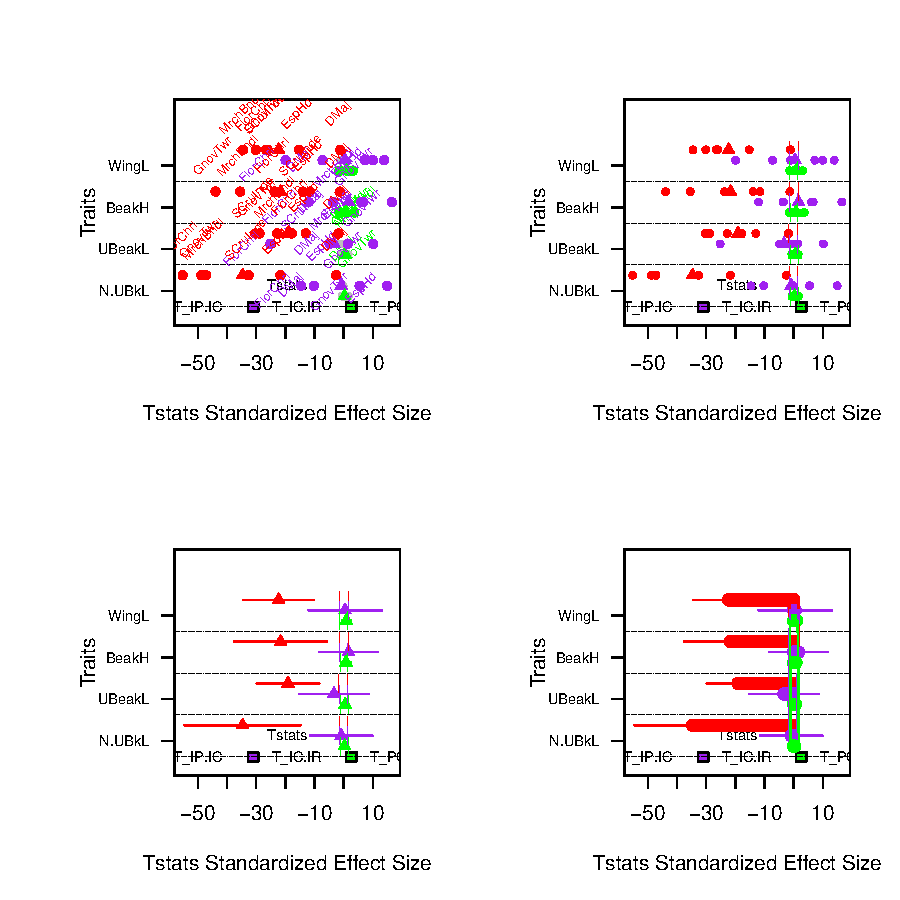
\includegraphics[width=\maxwidth]{figure/unnamed-chunk-22} 

}


\begin{kframe}\begin{alltt}
\hlkwd{par}\hlstd{(oldpar)}
\end{alltt}
\end{kframe}
\end{knitrout}


\newpage

\begin{knitrout}
\definecolor{shadecolor}{rgb}{0.969, 0.969, 0.969}\color{fgcolor}\begin{kframe}
\begin{alltt}
\hlkwd{barplot}\hlstd{(res.finch,} \hlkwc{ylim} \hlstd{=} \hlkwd{c}\hlstd{(}\hlnum{0}\hlstd{,} \hlnum{3.5}\hlstd{))}
\end{alltt}
\end{kframe}

{\centering 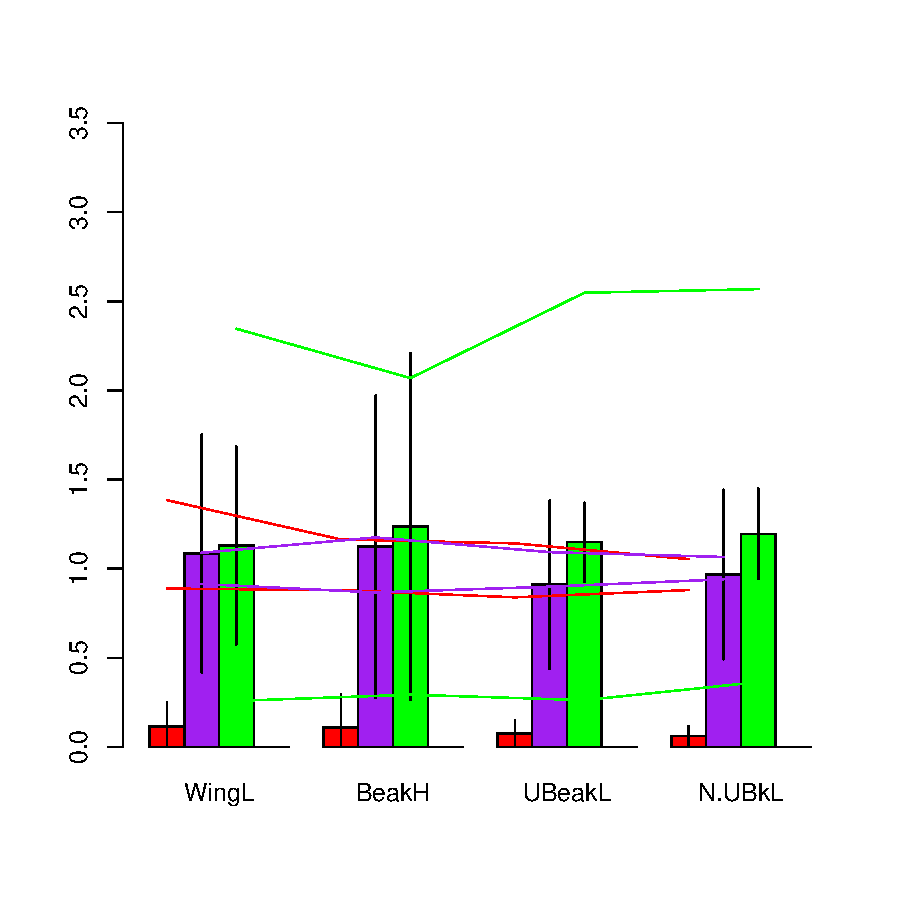
\includegraphics[width=\maxwidth]{figure/unnamed-chunk-23} 

}



\end{knitrout}


\begin{knitrout}
\definecolor{shadecolor}{rgb}{0.969, 0.969, 0.969}\color{fgcolor}\begin{kframe}
\begin{alltt}
\hlkwd{attributes}\hlstd{(}\hlkwd{summary}\hlstd{(res.finch))}
\end{alltt}
\begin{verbatim}
## $names
## [1] "p.value" "percent" "sites"   "binary"
\end{verbatim}
\begin{alltt}
\hlkwd{head}\hlstd{(}\hlkwd{summary}\hlstd{(res.finch)}\hlopt{$}\hlstd{p.value,} \hlnum{10}\hlstd{)}
\end{alltt}
\begin{verbatim}
##             WingL BeakH UBeakL N.UBkL
## T_IP.IC.inf   0.1   0.1    0.1    0.1
## T_IP.IC.inf   0.1   0.1    0.1    0.1
## T_IP.IC.inf   0.1   0.1    0.1    0.1
## T_IP.IC.inf   0.1   0.1    0.1    0.1
## T_IP.IC.inf   0.1   0.1    0.1    0.1
## T_IP.IC.inf   0.1   0.1    0.1    0.1
## T_IP.IC.sup   1.0   1.0    1.0    1.0
## T_IP.IC.sup   1.0   1.0    1.0    1.0
## T_IP.IC.sup   1.0   1.0    1.0    1.0
## T_IP.IC.sup   1.0   1.0    1.0    1.0
\end{verbatim}
\end{kframe}
\end{knitrout}


\newpage

We can also see T-statistics correlations and theirs correlation with others variables (e.g. a gradient variable, or the species richness).

\begin{knitrout}
\definecolor{shadecolor}{rgb}{0.969, 0.969, 0.969}\color{fgcolor}\begin{kframe}
\begin{alltt}
\hlkwd{par}\hlstd{(}\hlkwc{mfrow} \hlstd{=} \hlkwd{c}\hlstd{(}\hlnum{2}\hlstd{,} \hlnum{3}\hlstd{))}
\hlkwd{plot_cor.Tstats}\hlstd{(res.finch,} \hlkwc{plot.ask} \hlstd{=} \hlnum{FALSE}\hlstd{,} \hlkwc{multipanel} \hlstd{= F)}
\end{alltt}


{\ttfamily\noindent\color{warningcolor}{\#\# Warning: largeur de police inconnue pour le caractère 0xd\\\#\# Warning: largeur de police inconnue pour le caractère 0xd}}\end{kframe}
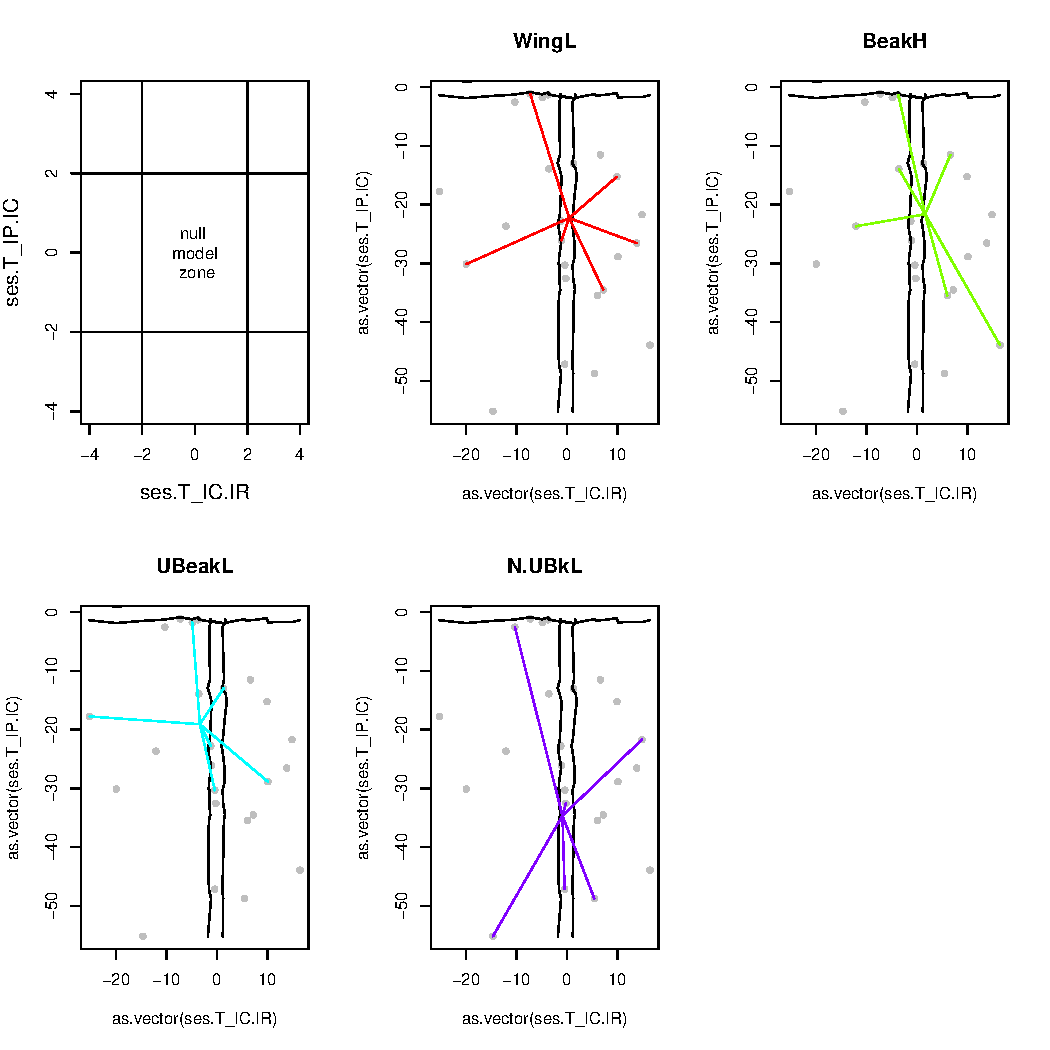
\includegraphics[width=\maxwidth]{figure/unnamed-chunk-251} 
\begin{kframe}

{\ttfamily\noindent\color{warningcolor}{\#\# Warning: largeur de police inconnue pour le caractère 0xd\\\#\# Warning: largeur de police inconnue pour le caractère 0xd}}\end{kframe}
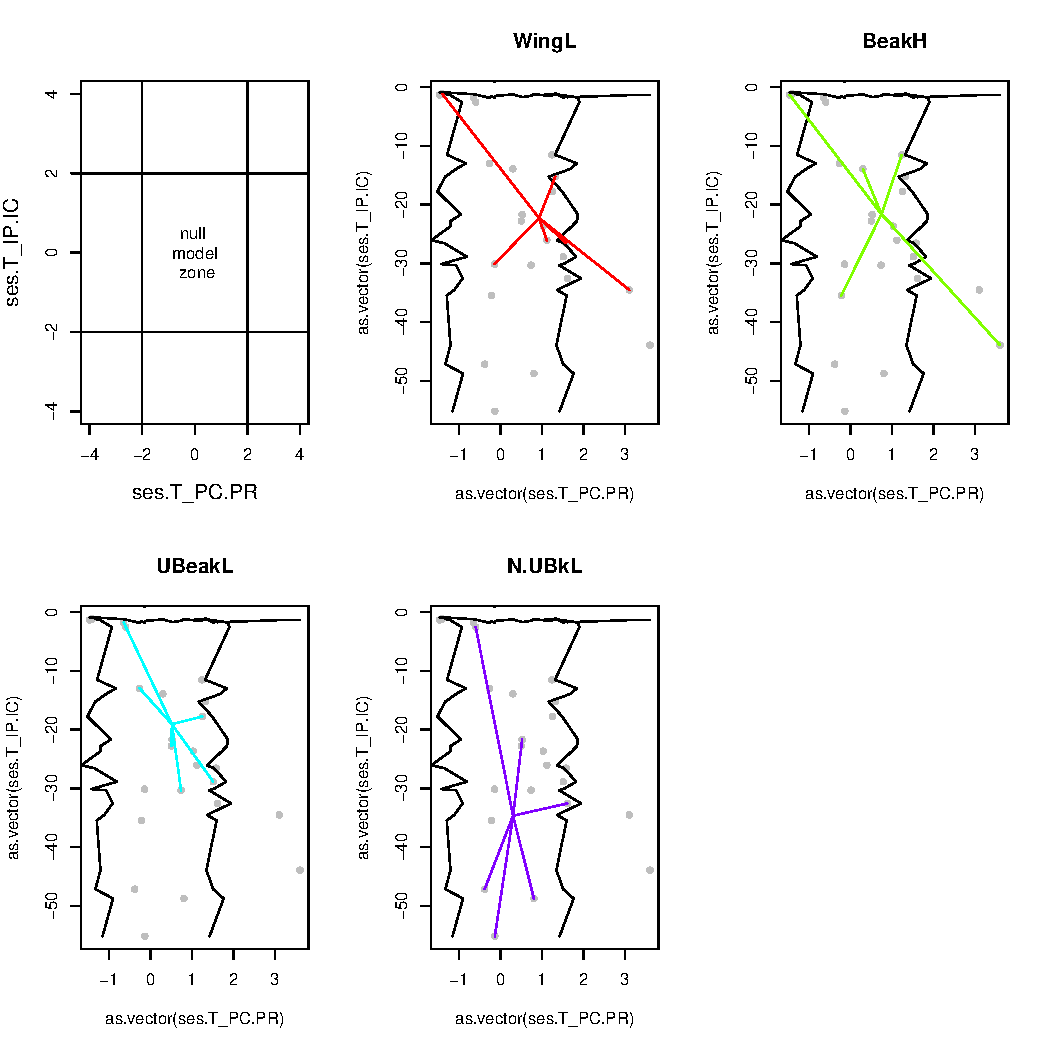
\includegraphics[width=\maxwidth]{figure/unnamed-chunk-252} 
\begin{kframe}

{\ttfamily\noindent\color{warningcolor}{\#\# Warning: largeur de police inconnue pour le caractère 0xd\\\#\# Warning: largeur de police inconnue pour le caractère 0xd}}\end{kframe}
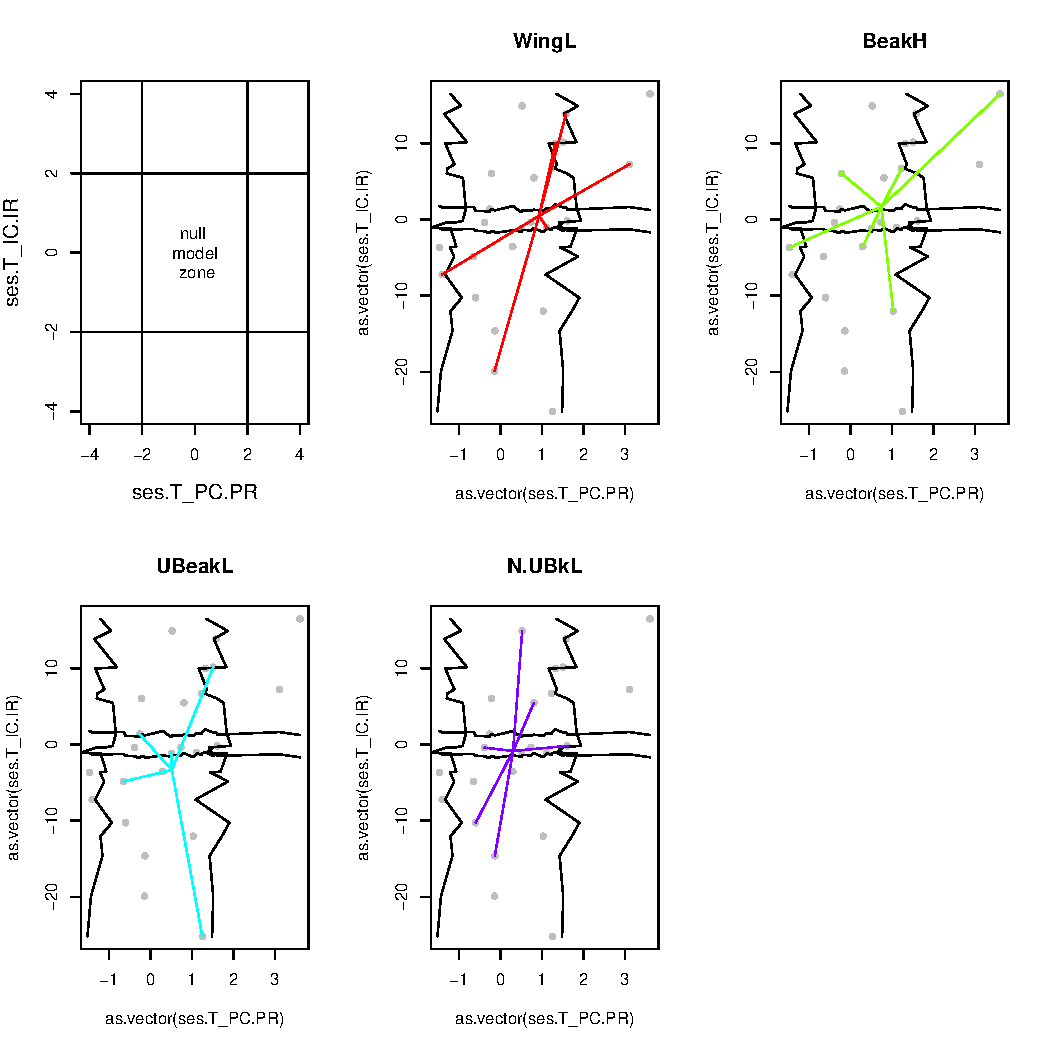
\includegraphics[width=\maxwidth]{figure/unnamed-chunk-253} 

\end{knitrout}


Here we plot T-statistics in function of species richness by sites.

\begin{knitrout}
\definecolor{shadecolor}{rgb}{0.969, 0.969, 0.969}\color{fgcolor}\begin{kframe}
\begin{alltt}
\hlkwd{par}\hlstd{(}\hlkwc{mfrow} \hlstd{=} \hlkwd{c}\hlstd{(}\hlnum{2}\hlstd{,} \hlnum{2}\hlstd{))}
\hlstd{species.richness} \hlkwb{<-} \hlkwd{table}\hlstd{(ind.plot.finch)}
\hlkwd{plot_ses.var}\hlstd{(}\hlkwd{as.listofindex}\hlstd{(}\hlkwd{list}\hlstd{(res.finch)), species.richness,} \hlkwc{multipanel} \hlstd{= F)}
\end{alltt}
\end{kframe}
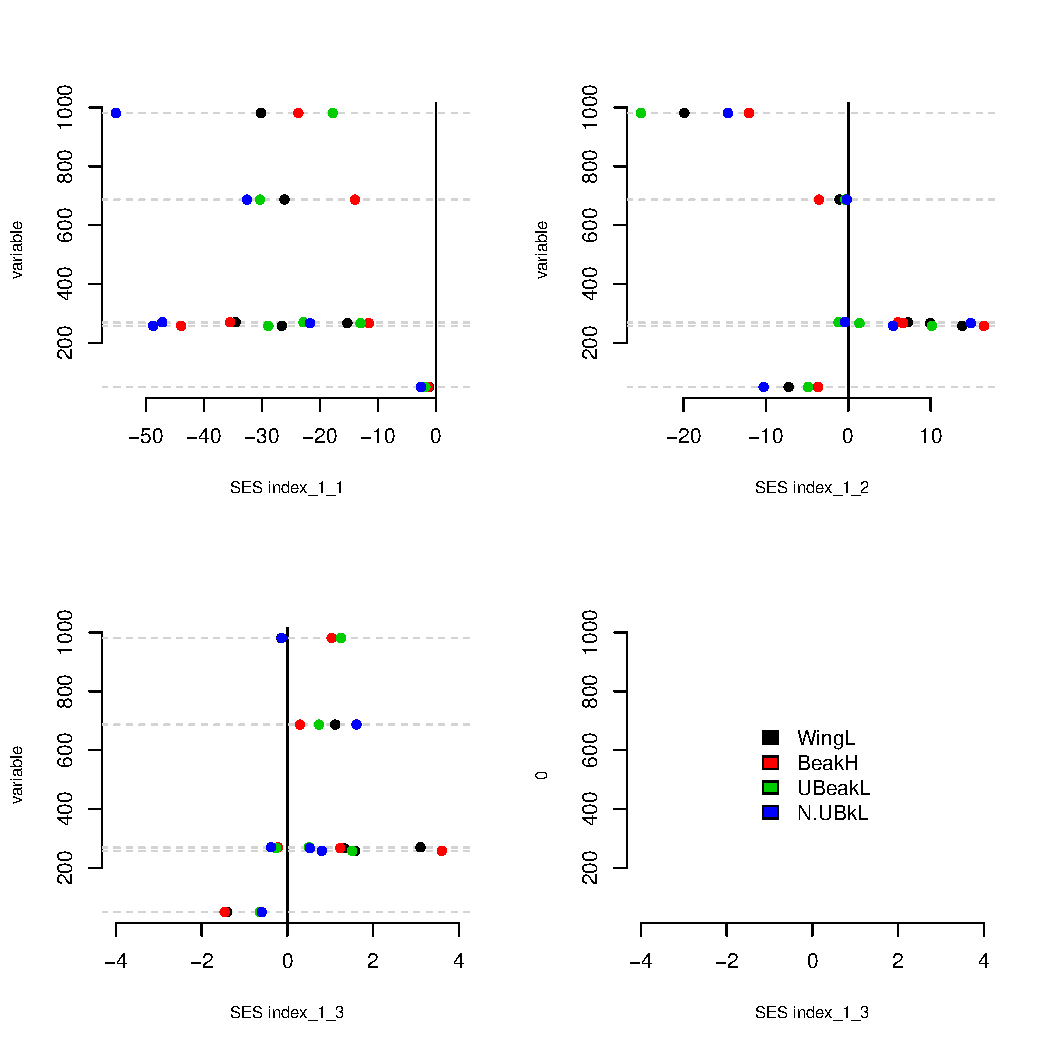
\includegraphics[width=\maxwidth]{figure/unnamed-chunk-26} 

\end{knitrout}


Same plot with \code(resume=TRUE).

\begin{knitrout}
\definecolor{shadecolor}{rgb}{0.969, 0.969, 0.969}\color{fgcolor}\begin{kframe}
\begin{alltt}
\hlkwd{par}\hlstd{(}\hlkwc{mfrow} \hlstd{=} \hlkwd{c}\hlstd{(}\hlnum{2}\hlstd{,} \hlnum{2}\hlstd{))}
\hlkwd{plot_ses.var}\hlstd{(}\hlkwd{as.listofindex}\hlstd{(}\hlkwd{list}\hlstd{(res.finch)), species.richness,} \hlkwc{resume} \hlstd{= T,}
    \hlkwc{multipanel} \hlstd{= F)}
\end{alltt}
\end{kframe}
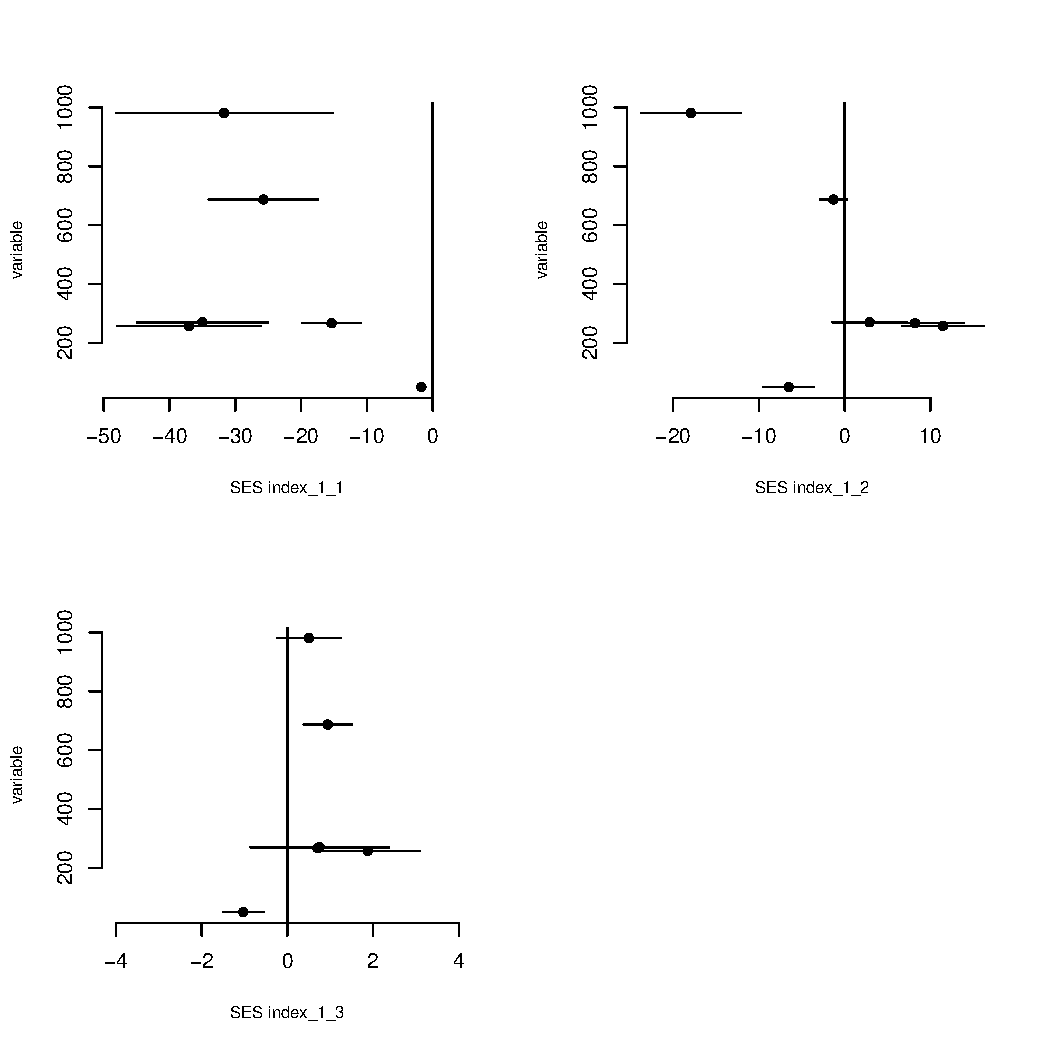
\includegraphics[width=\maxwidth]{figure/unnamed-chunk-27} 
\begin{kframe}\begin{alltt}
\hlkwd{par}\hlstd{(}\hlkwc{mfrow} \hlstd{=} \hlkwd{c}\hlstd{(}\hlnum{1}\hlstd{,} \hlnum{1}\hlstd{))}
\end{alltt}
\end{kframe}
\end{knitrout}



\newpage
\subsection{Others univariates index}

The function \code(com.index) allow to choose your own function (like mean, range, variance...) to calculate customize index.

\begin{knitrout}
\definecolor{shadecolor}{rgb}{0.969, 0.969, 0.969}\color{fgcolor}\begin{kframe}
\begin{alltt}
\hlstd{funct} \hlkwb{<-} \hlkwd{c}\hlstd{(}\hlstr{"mean(x, na.rm=T)"}\hlstd{,} \hlstr{"kurtosis(x, na.rm=T)"}\hlstd{,} \hlstr{"max(x, na.rm=T) - min(x, na.rm=T)"}\hlstd{,}
    \hlstr{"CVNND(x)"}\hlstd{)}
\hlstd{res.finch.sp_mn2} \hlkwb{<-} \hlkwd{com.index}\hlstd{(}\hlkwc{traits} \hlstd{= traits.finch,} \hlkwc{index} \hlstd{= funct,} \hlkwc{sp} \hlstd{= sp.finch,}
    \hlkwc{nullmodels} \hlstd{=} \hlkwd{c}\hlstd{(}\hlnum{2}\hlstd{,} \hlnum{2}\hlstd{,} \hlnum{2}\hlstd{,} \hlnum{2}\hlstd{),} \hlkwc{ind.plot} \hlstd{= ind.plot.finch,} \hlkwc{nperm} \hlstd{=} \hlnum{9}\hlstd{,} \hlkwc{print} \hlstd{=} \hlnum{FALSE}\hlstd{)}
\hlstd{res.finch.sp_mn3} \hlkwb{<-} \hlkwd{com.index}\hlstd{(}\hlkwc{traits} \hlstd{= traits.finch,} \hlkwc{index} \hlstd{= funct,} \hlkwc{sp} \hlstd{= sp.finch,}
    \hlkwc{nullmodels} \hlstd{=} \hlkwd{c}\hlstd{(}\hlnum{3}\hlstd{,} \hlnum{3}\hlstd{,} \hlnum{3}\hlstd{,} \hlnum{3}\hlstd{),} \hlkwc{ind.plot} \hlstd{= ind.plot.finch,} \hlkwc{nperm} \hlstd{=} \hlnum{9}\hlstd{,} \hlkwc{print} \hlstd{=} \hlnum{FALSE}\hlstd{)}
\end{alltt}
\end{kframe}
\end{knitrout}


\newpage
We can represent Standardized Effect Size (ses) using the function \code(plot(as.listofindex(list1, list2, list3)))
\begin{knitrout}
\definecolor{shadecolor}{rgb}{0.969, 0.969, 0.969}\color{fgcolor}\begin{kframe}
\begin{alltt}
\hlstd{list.ind2} \hlkwb{<-} \hlkwd{list}\hlstd{(res.finch.sp_mn2, res.finch.sp_mn3)}
\hlstd{index.list2} \hlkwb{<-} \hlkwd{as.listofindex}\hlstd{(list.ind2)}

\hlkwd{plot}\hlstd{(index.list2)}
\end{alltt}
\end{kframe}
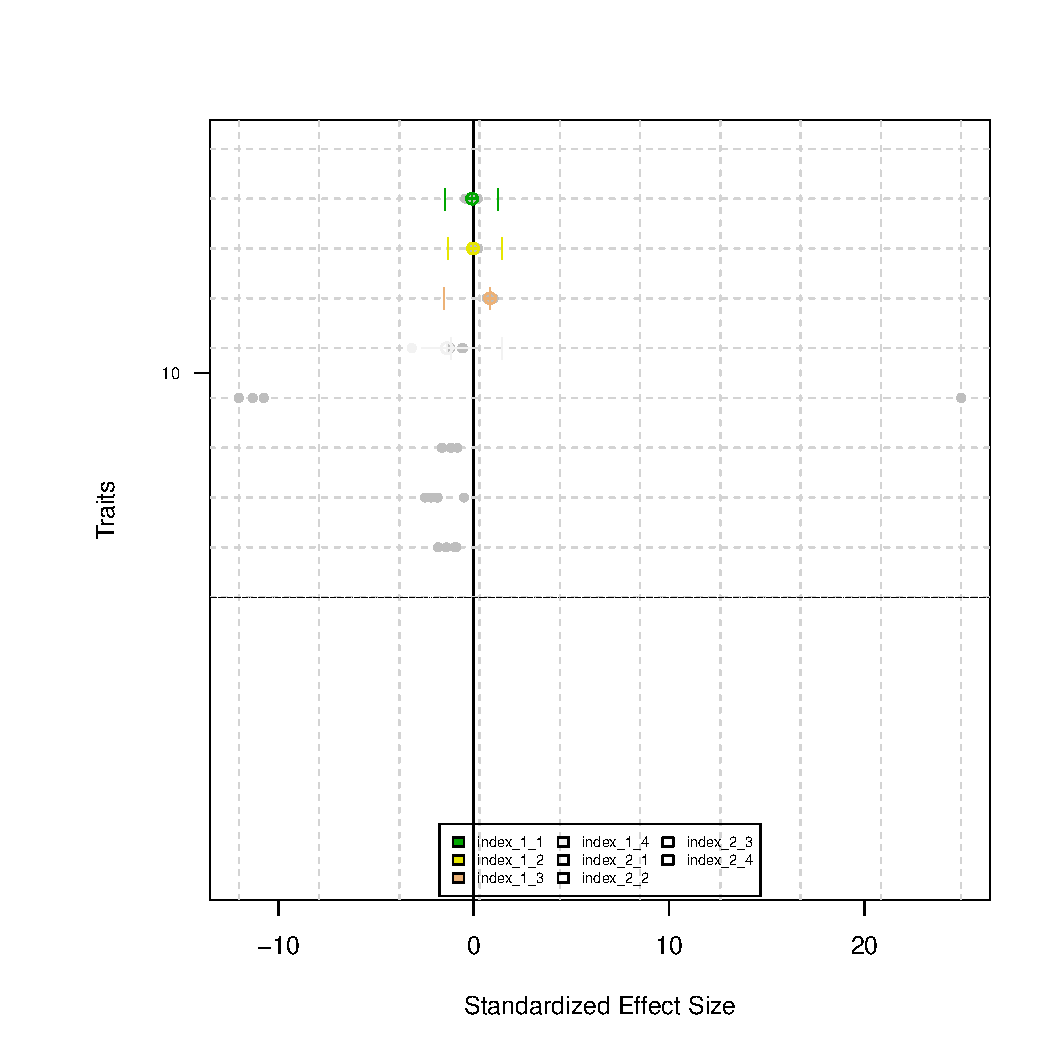
\includegraphics[width=\maxwidth]{figure/unnamed-chunk-29} 

\end{knitrout}


\newpage

This allows to calcul index by sites for example using \code("tapply(x, sites, mean)").

\begin{knitrout}
\definecolor{shadecolor}{rgb}{0.969, 0.969, 0.969}\color{fgcolor}\begin{kframe}
\begin{alltt}
\hlstd{funct} \hlkwb{<-} \hlkwd{c}\hlstd{(}\hlstr{"tapply(x, ind.plot.finch, function(x) mean(x, na.rm=T))"}\hlstd{,} \hlstr{"tapply(x, ind.plot.finch, function(x) kurtosis(x, na.rm=T))"}\hlstd{,}
    \hlstr{"tapply(x, ind.plot.finch, function(x) max(x, na.rm=T)-min(x, na.rm=T))"}\hlstd{,}
    \hlstr{"tapply(x, ind.plot.finch, function(x) CVNND(x))"}\hlstd{)}

\hlcom{## Null model 1 is trivial for this function because randomisation is within}
\hlcom{## community only}

\hlstd{res.finch.ind_mn1} \hlkwb{<-} \hlkwd{com.index}\hlstd{(}\hlkwc{traits} \hlstd{= traits.finch,} \hlkwc{index} \hlstd{= funct,} \hlkwc{sp} \hlstd{= sp.finch,}
    \hlkwc{nullmodels} \hlstd{=} \hlkwd{c}\hlstd{(}\hlnum{1}\hlstd{,} \hlnum{1}\hlstd{,} \hlnum{1}\hlstd{,} \hlnum{1}\hlstd{),} \hlkwc{ind.plot} \hlstd{= ind.plot.finch,} \hlkwc{nperm} \hlstd{=} \hlnum{9}\hlstd{,} \hlkwc{print} \hlstd{=} \hlnum{FALSE}\hlstd{)}
\hlstd{res.finch.ind_mn2} \hlkwb{<-} \hlkwd{com.index}\hlstd{(}\hlkwc{traits} \hlstd{= traits.finch,} \hlkwc{index} \hlstd{= funct,} \hlkwc{sp} \hlstd{= sp.finch,}
    \hlkwc{nullmodels} \hlstd{=} \hlkwd{c}\hlstd{(}\hlnum{2}\hlstd{,} \hlnum{2}\hlstd{,} \hlnum{2}\hlstd{,} \hlnum{2}\hlstd{),} \hlkwc{ind.plot} \hlstd{= ind.plot.finch,} \hlkwc{nperm} \hlstd{=} \hlnum{9}\hlstd{,} \hlkwc{print} \hlstd{=} \hlnum{FALSE}\hlstd{)}
\end{alltt}
\end{kframe}
\end{knitrout}



We can calcul index with or without intraspecific variance.

\begin{knitrout}
\definecolor{shadecolor}{rgb}{0.969, 0.969, 0.969}\color{fgcolor}\begin{kframe}
\begin{alltt}
\hlcom{# Calcul of means by population (name_sp_site is a name of a population)}
\hlcom{# like in the function com.index and determine the site for each population}
\hlcom{# (sites_bypop)}

\hlstd{name_sp_sites} \hlkwb{=} \hlkwd{paste}\hlstd{(sp.finch, ind.plot.finch,} \hlkwc{sep} \hlstd{=} \hlstr{"_"}\hlstd{)}
\hlstd{traits.by.pop} \hlkwb{<-} \hlkwd{apply}\hlstd{(traits.finch,} \hlnum{2}\hlstd{,} \hlkwa{function}\hlstd{(}\hlkwc{x}\hlstd{)} \hlkwd{tapply}\hlstd{(x, name_sp_sites,}
    \hlstd{mean,} \hlkwc{na.rm} \hlstd{= T))}

\hlstd{sites_bypop} \hlkwb{<-} \hlkwd{lapply}\hlstd{(}\hlkwd{strsplit}\hlstd{(}\hlkwd{paste}\hlstd{(}\hlkwd{rownames}\hlstd{(traits.by.pop),} \hlkwc{sep} \hlstd{=} \hlstr{"_"}\hlstd{),} \hlkwc{split} \hlstd{=} \hlstr{"_"}\hlstd{),}
    \hlkwa{function}\hlstd{(}\hlkwc{x}\hlstd{) x[}\hlnum{3}\hlstd{])}

\hlcom{# We use the precedent list of function 'funct'}
\hlstd{funct.withIV} \hlkwb{<-} \hlstd{funct}

\hlstd{fact} \hlkwb{<-} \hlkwd{unlist}\hlstd{(sites_bypop)}
\hlstd{funct.withoutIV} \hlkwb{<-} \hlkwd{c}\hlstd{(}\hlstr{"tapply(x, fact, function(x) mean(x, na.rm=T))"}\hlstd{,} \hlstr{"tapply(x, fact, function(x) kurtosis(x, na.rm=T))"}\hlstd{,}
    \hlstr{"tapply(x, fact, function(x) max(x, na.rm=T)-min(x, na.rm=T))"}\hlstd{,} \hlstr{"tapply(x, fact, function(x) CVNND(x))"}\hlstd{)}


\hlstd{res.finch.withIV} \hlkwb{<-} \hlkwd{com.index}\hlstd{(}\hlkwc{traits} \hlstd{= traits.finch,} \hlkwc{index} \hlstd{= funct.withIV,} \hlkwc{sp} \hlstd{= sp.finch,}
    \hlkwc{nullmodels} \hlstd{=} \hlkwd{c}\hlstd{(}\hlnum{2}\hlstd{,} \hlnum{2}\hlstd{,} \hlnum{2}\hlstd{,} \hlnum{2}\hlstd{),} \hlkwc{ind.plot} \hlstd{= ind.plot.finch,} \hlkwc{nperm} \hlstd{=} \hlnum{9}\hlstd{,} \hlkwc{print} \hlstd{=} \hlnum{FALSE}\hlstd{)}

\hlstd{res.finch.withoutIV} \hlkwb{<-} \hlkwd{com.index}\hlstd{(}\hlkwc{traits} \hlstd{= traits.finch,} \hlkwc{index} \hlstd{= funct.withoutIV,}
    \hlkwc{sp} \hlstd{= sp.finch,} \hlkwc{nullmodels} \hlstd{=} \hlkwd{c}\hlstd{(}\hlnum{3}\hlstd{,} \hlnum{3}\hlstd{,} \hlnum{3}\hlstd{,} \hlnum{3}\hlstd{),} \hlkwc{ind.plot} \hlstd{= ind.plot.finch,} \hlkwc{nperm} \hlstd{=} \hlnum{9}\hlstd{,}
    \hlkwc{print} \hlstd{=} \hlnum{FALSE}\hlstd{)}
\end{alltt}
\end{kframe}
\end{knitrout}



\newpage

We can also represent T-statistics and custom index thanks to the \code(plot.listofindex) function.
\begin{knitrout}
\definecolor{shadecolor}{rgb}{0.969, 0.969, 0.969}\color{fgcolor}\begin{kframe}
\begin{alltt}
\hlstd{list.ind} \hlkwb{<-} \hlkwd{list}\hlstd{(res.finch.withIV, res.finch.withoutIV, res.finch)}
\hlstd{namesindex.i.l1} \hlkwb{=} \hlkwd{c}\hlstd{(}\hlstr{"mean"}\hlstd{,} \hlstr{"kurtosis"}\hlstd{,} \hlstr{"range"}\hlstd{,} \hlstr{"CVNND"}\hlstd{,} \hlstr{"mean.pop"}\hlstd{,} \hlstr{"kurtosis.pop"}\hlstd{,}
    \hlstr{"range.pop"}\hlstd{,} \hlstr{"CVNND.pop"}\hlstd{,} \hlstr{"T_IP.IC"}\hlstd{,} \hlstr{"T_IC.IR"}\hlstd{,} \hlstr{"T_PC.PR"}\hlstd{)}

\hlstd{i.l1} \hlkwb{<-} \hlkwd{as.listofindex}\hlstd{(list.ind,} \hlkwc{namesindex} \hlstd{= namesindex.i.l1)}

\hlkwd{class}\hlstd{(i.l1)}
\end{alltt}
\begin{verbatim}
## [1] "listofindex"
\end{verbatim}
\begin{alltt}
\hlkwd{par}\hlstd{(}\hlkwc{mfrow} \hlstd{=} \hlkwd{c}\hlstd{(}\hlnum{2}\hlstd{,} \hlnum{3}\hlstd{))}
\hlkwd{plot}\hlstd{(i.l1,} \hlkwc{type} \hlstd{=} \hlstr{"bytraits"}\hlstd{,} \hlkwc{bysites} \hlstd{=} \hlnum{TRUE}\hlstd{)}
\end{alltt}


{\ttfamily\noindent\color{warningcolor}{\#\# Warning: "{}bysites"{} is not a graphical parameter\\\#\# Warning: "{}bysites"{} is not a graphical parameter\\\#\# Warning: "{}bysites"{} is not a graphical parameter\\\#\# Warning: "{}bysites"{} is not a graphical parameter\\\#\# Warning: "{}bysites"{} is not a graphical parameter\\\#\# Warning: "{}bysites"{} is not a graphical parameter\\\#\# Warning: "{}bysites"{} is not a graphical parameter\\\#\# Warning: "{}bysites"{} is not a graphical parameter\\\#\# Warning: "{}bysites"{} is not a graphical parameter\\\#\# Warning: "{}bysites"{} is not a graphical parameter\\\#\# Warning: "{}bysites"{} is not a graphical parameter\\\#\# Warning: "{}bysites"{} is not a graphical parameter\\\#\# Warning: "{}bysites"{} is not a graphical parameter\\\#\# Warning: "{}bysites"{} is not a graphical parameter\\\#\# Warning: "{}bysites"{} is not a graphical parameter\\\#\# Warning: "{}bysites"{} is not a graphical parameter\\\#\# Warning: "{}bysites"{} is not a graphical parameter\\\#\# Warning: "{}bysites"{} is not a graphical parameter\\\#\# Warning: "{}bysites"{} is not a graphical parameter\\\#\# Warning: "{}bysites"{} is not a graphical parameter\\\#\# Warning: "{}bysites"{} is not a graphical parameter\\\#\# Warning: "{}bysites"{} is not a graphical parameter\\\#\# Warning: "{}bysites"{} is not a graphical parameter\\\#\# Warning: "{}bysites"{} is not a graphical parameter}}\end{kframe}
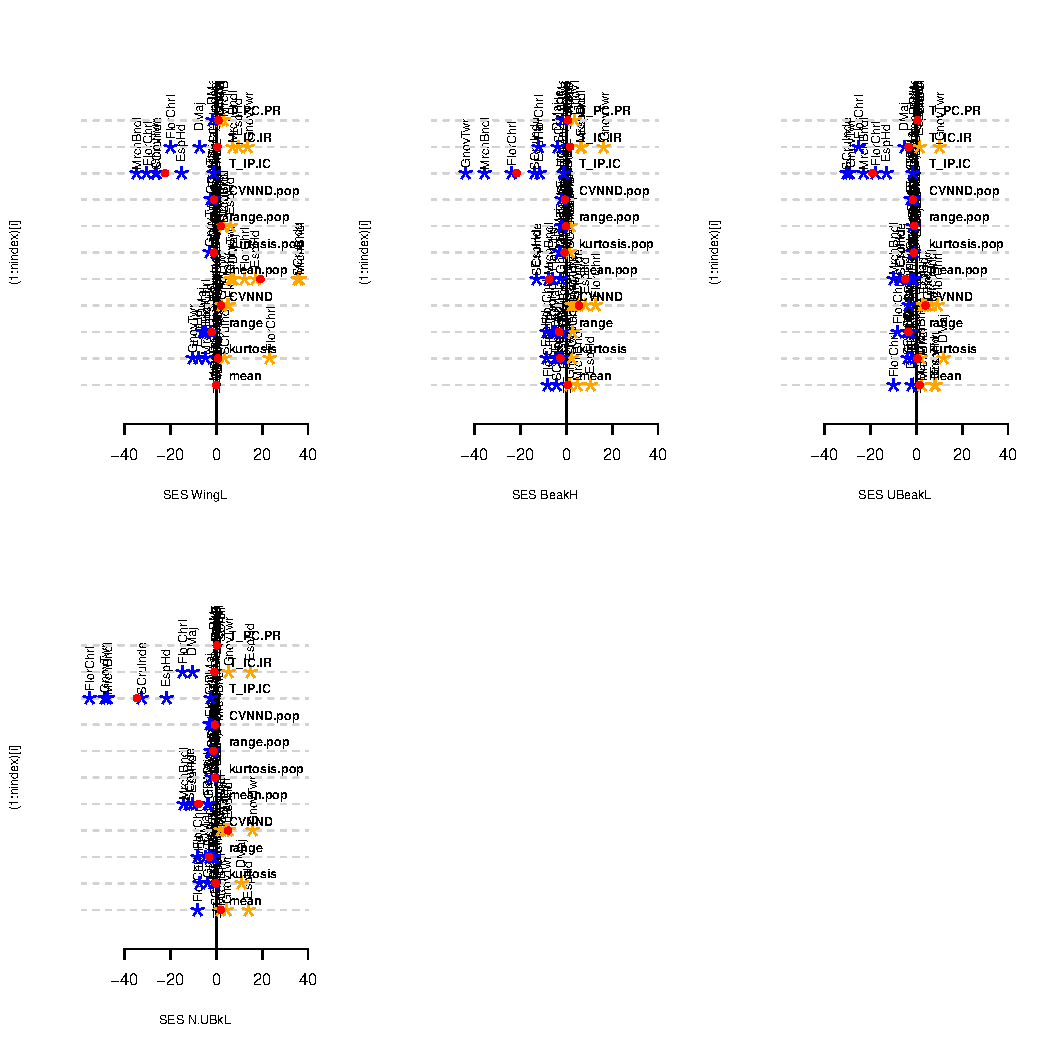
\includegraphics[width=\maxwidth]{figure/unnamed-chunk-321} 
\begin{kframe}\begin{alltt}
\hlkwd{par}\hlstd{(}\hlkwc{mfrow} \hlstd{=} \hlkwd{c}\hlstd{(}\hlnum{2}\hlstd{,} \hlnum{2}\hlstd{))}
\hlkwd{plot}\hlstd{(i.l1,} \hlkwc{type} \hlstd{=} \hlstr{"bytraits"}\hlstd{)}
\end{alltt}
\end{kframe}
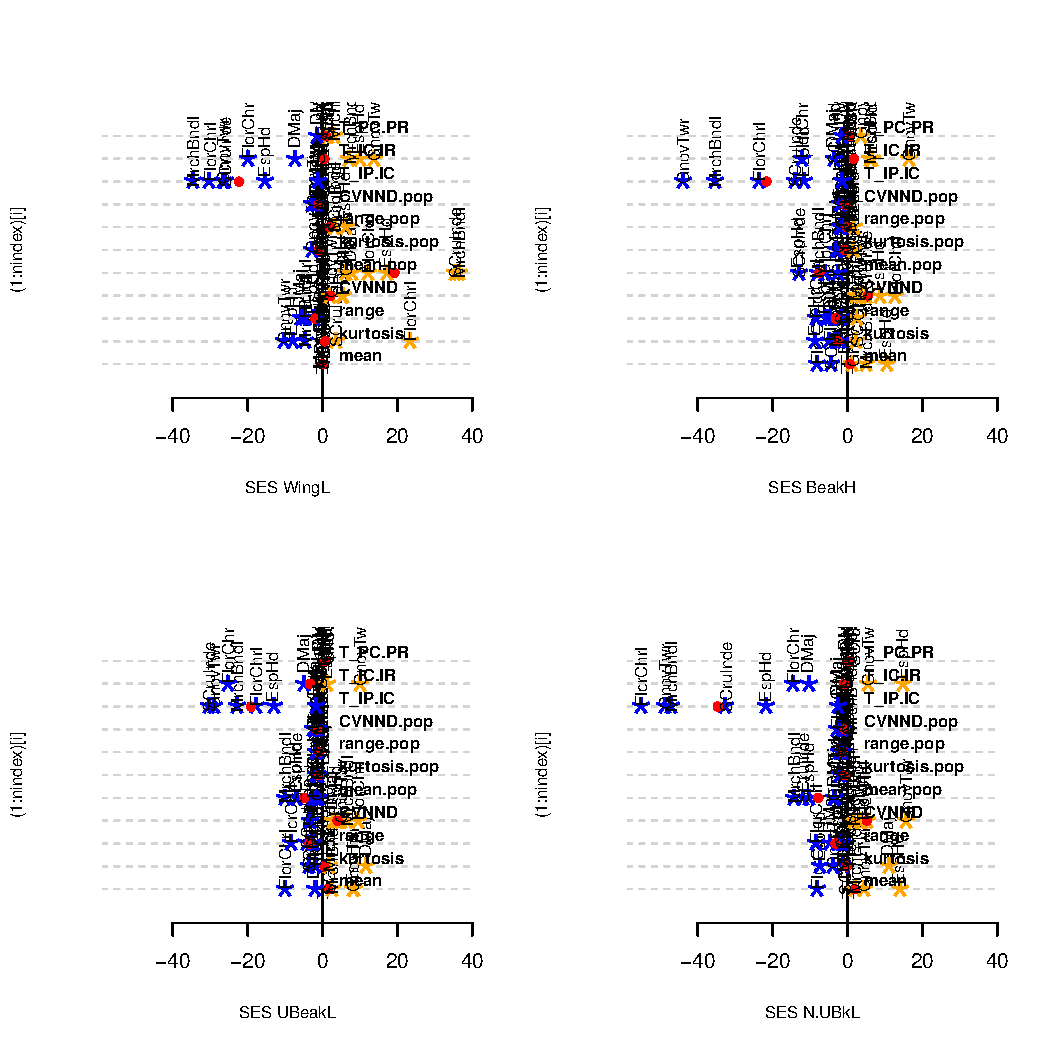
\includegraphics[width=\maxwidth]{figure/unnamed-chunk-322} 
\begin{kframe}\begin{alltt}
\hlkwd{par}\hlstd{(}\hlkwc{mfrow} \hlstd{=} \hlkwd{c}\hlstd{(}\hlnum{1}\hlstd{,} \hlnum{1}\hlstd{))}
\end{alltt}
\end{kframe}
\end{knitrout}



\begin{knitrout}
\definecolor{shadecolor}{rgb}{0.969, 0.969, 0.969}\color{fgcolor}\begin{kframe}
\begin{alltt}
\hlkwd{plot}\hlstd{(i.l1,} \hlkwc{type} \hlstd{=} \hlstr{"simple"}\hlstd{)}
\end{alltt}
\end{kframe}
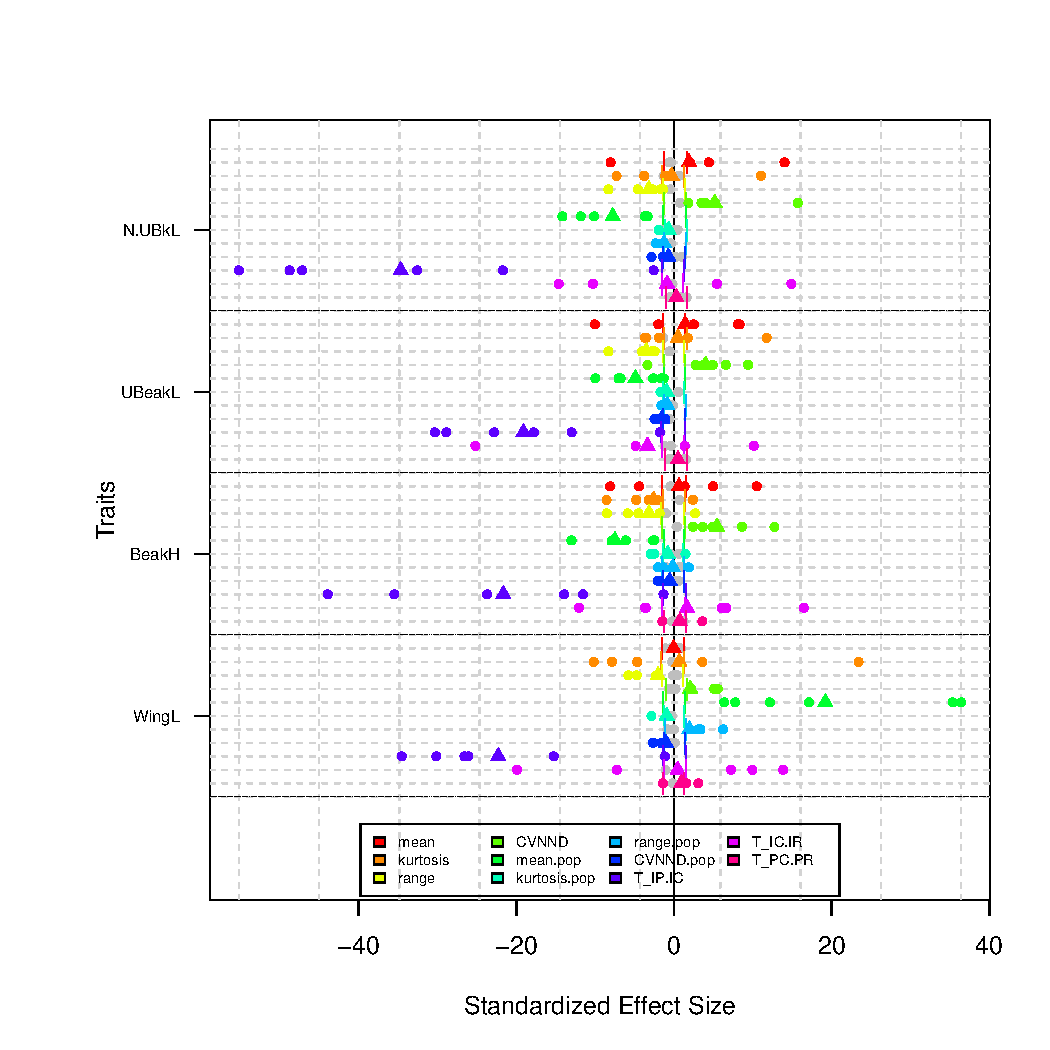
\includegraphics[width=\maxwidth]{figure/unnamed-chunk-331} 
\begin{kframe}\begin{alltt}
\hlkwd{plot}\hlstd{(i.l1,} \hlkwc{type} \hlstd{=} \hlstr{"simple_range"}\hlstd{)}
\end{alltt}
\end{kframe}
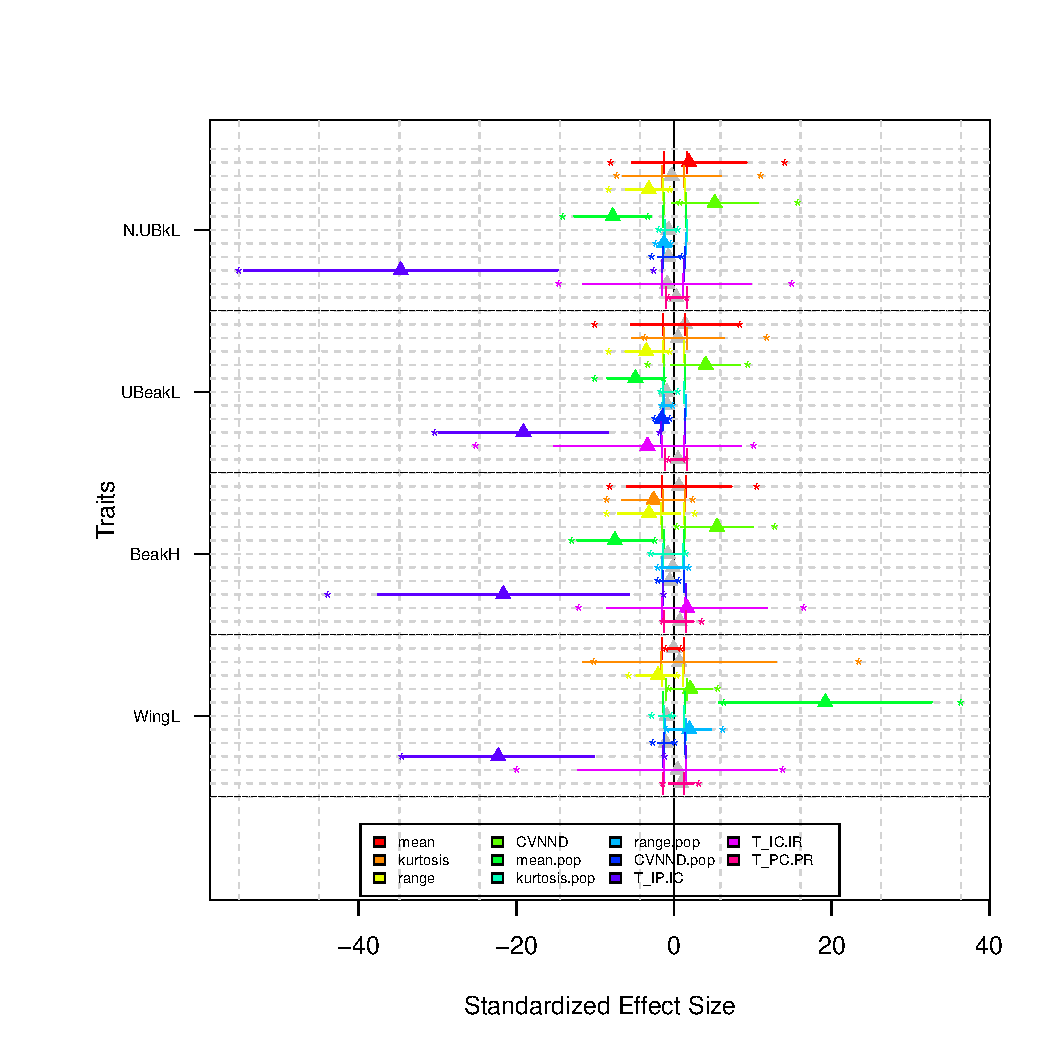
\includegraphics[width=\maxwidth]{figure/unnamed-chunk-332} 
\begin{kframe}\begin{alltt}
\hlkwd{plot}\hlstd{(i.l1,} \hlkwc{type} \hlstd{=} \hlstr{"normal"}\hlstd{)}
\end{alltt}
\end{kframe}
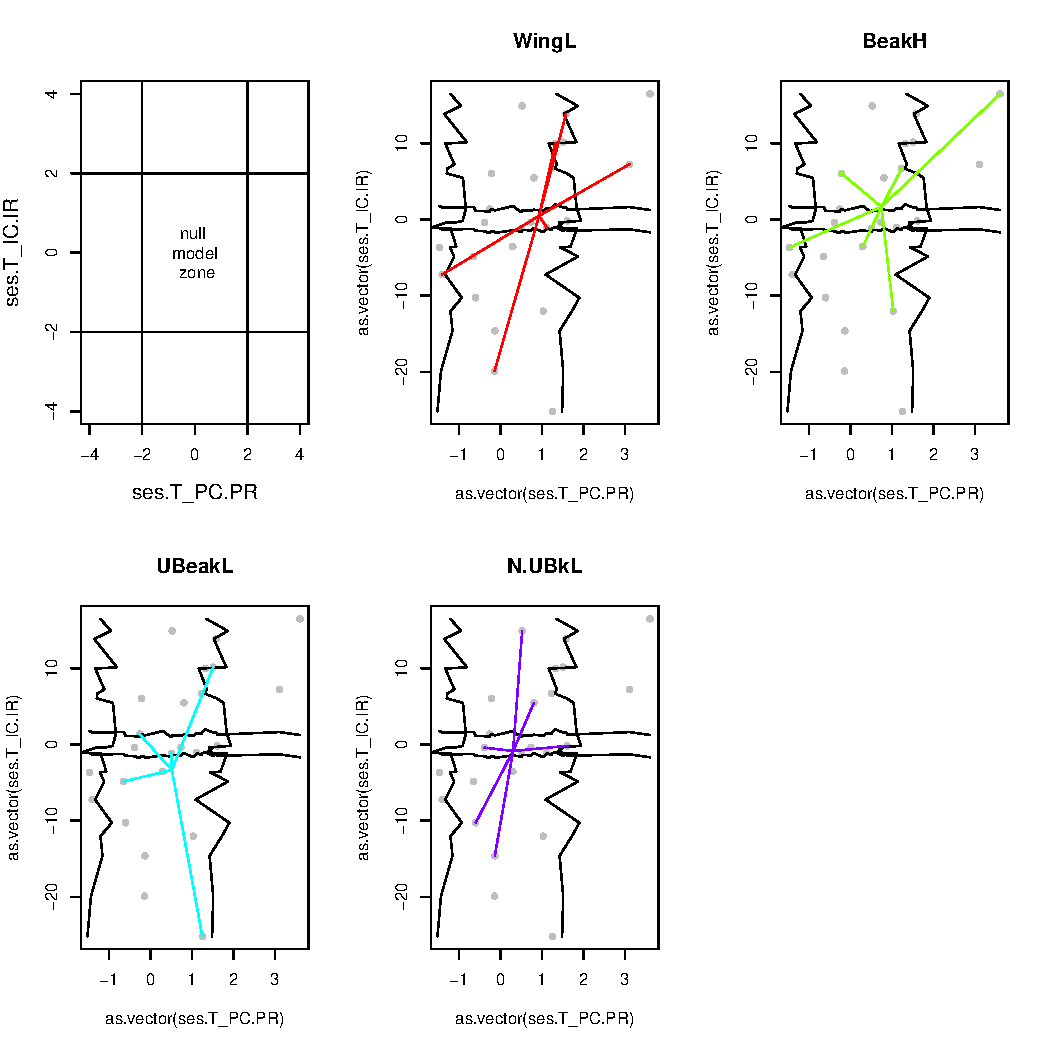
\includegraphics[width=\maxwidth]{figure/unnamed-chunk-333} 
\begin{kframe}\begin{alltt}
\hlkwd{plot}\hlstd{(i.l1,} \hlkwc{type} \hlstd{=} \hlstr{"barplot"}\hlstd{)}
\end{alltt}
\end{kframe}
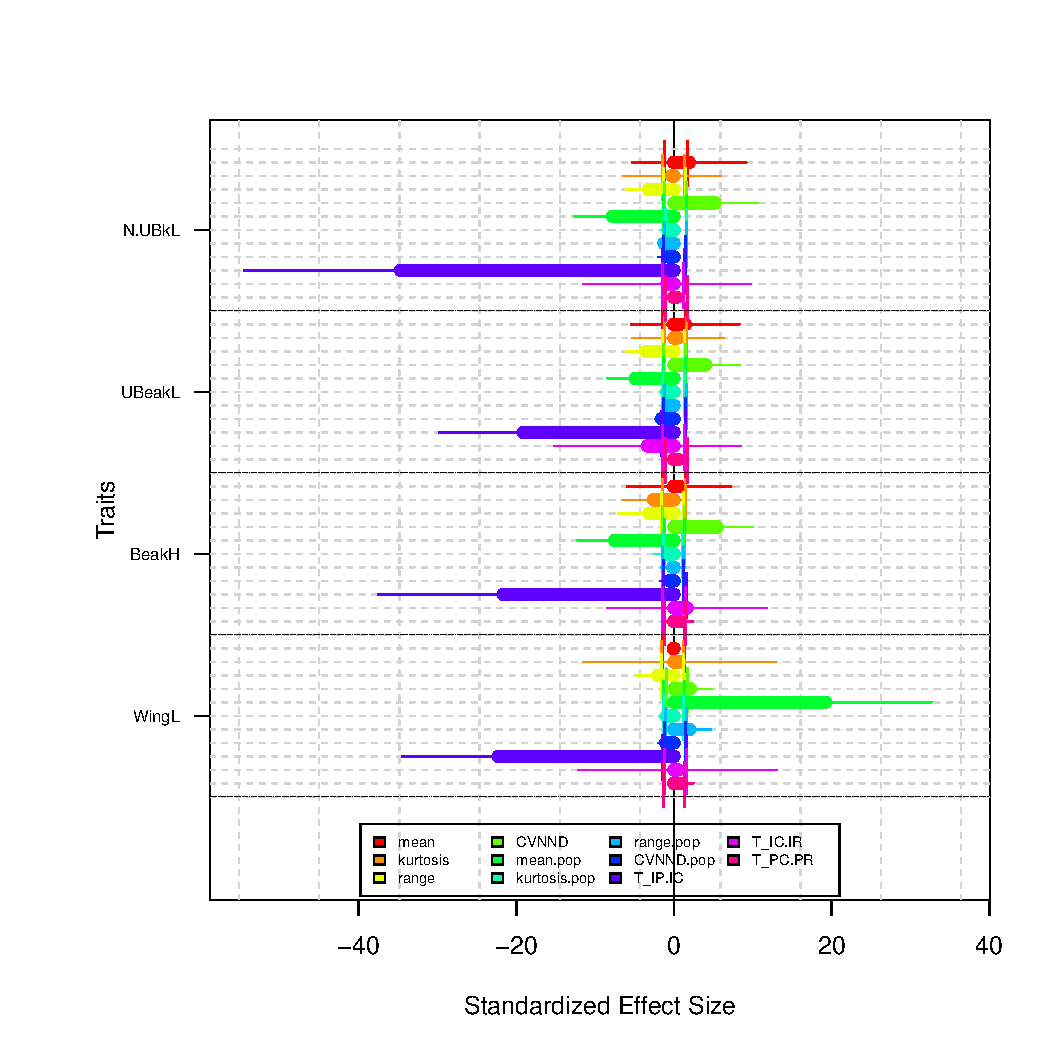
\includegraphics[width=\maxwidth]{figure/unnamed-chunk-334} 

\end{knitrout}




\newpage

\subsection{Multivariates index}

For most multivariate functions we need to replace (or exclude) NA values. For this example, we use the package mice to complete the data.

\begin{knitrout}
\definecolor{shadecolor}{rgb}{0.969, 0.969, 0.969}\color{fgcolor}\begin{kframe}
\begin{alltt}
\hlstd{comm} \hlkwb{<-} \hlkwd{t}\hlstd{(}\hlkwd{table}\hlstd{(ind.plot.finch,} \hlnum{1}\hlopt{:}\hlkwd{length}\hlstd{(ind.plot.finch)))}

\hlkwd{require}\hlstd{(mice)}
\hlstd{traits} \hlkwb{=} \hlstd{traits.finch}
\hlstd{mice} \hlkwb{<-} \hlkwd{mice}\hlstd{(traits.finch)}
\hlstd{traits.finch.mice} \hlkwb{<-} \hlkwd{complete}\hlstd{(mice)}
\end{alltt}
\end{kframe}
\end{knitrout}


A simple example to illustrate the concept of the function \code(com.index.multi) 

\begin{knitrout}
\definecolor{shadecolor}{rgb}{0.969, 0.969, 0.969}\color{fgcolor}\begin{kframe}
\begin{alltt}
\hlstd{n_sp_plot} \hlkwb{<-} \hlkwd{as.factor}\hlstd{(}\hlkwd{paste}\hlstd{(sp.finch, ind.plot.finch,} \hlkwc{sep} \hlstd{=} \hlstr{"_"}\hlstd{))}
\hlstd{res.sum.1} \hlkwb{<-} \hlkwd{com.index.multi}\hlstd{(traits.finch,} \hlkwc{index} \hlstd{=} \hlkwd{c}\hlstd{(}\hlstr{"sum(scale(x), na.rm=T)"}\hlstd{,}
    \hlstr{"sum(x, na.rm=T)"}\hlstd{),} \hlkwc{by.factor} \hlstd{= n_sp_plot,} \hlkwc{nullmodels} \hlstd{=} \hlkwd{c}\hlstd{(}\hlnum{2}\hlstd{,} \hlnum{2}\hlstd{),} \hlkwc{ind.plot} \hlstd{= ind.plot.finch,}
    \hlkwc{nperm} \hlstd{=} \hlnum{9}\hlstd{,} \hlkwc{sp} \hlstd{= sp.finch)}
\end{alltt}
\begin{verbatim}
## [1] "creating null models"
## [1] "nm.2 25 %"
## [1] "nm.2 50 %"
## [1] "nm.2 75 %"
## [1] "nm.2 100 %"
## [1] "calcul of null values using null models"
## [1] "sum(scale(x), na.rm=T) 50 %"
## [1] "sum(x, na.rm=T) 100 %"
## [1] "calcul of observed values"
## [1] "50 %"
## [1] "100 %"
\end{verbatim}
\begin{alltt}
\hlkwd{attributes}\hlstd{(}\hlkwd{ses.listofindex}\hlstd{(}\hlkwd{as.listofindex}\hlstd{(}\hlkwd{list}\hlstd{(res.sum.1))))}
\end{alltt}
\begin{verbatim}
## $names
## [1] "index_1_1" "index_1_2"
## 
## $class
## [1] "ses.list"
\end{verbatim}
\end{kframe}
\end{knitrout}


\newpage
A more interesting example using the function \code(hypervolume) from the package ... hypervolume.  We show here several results which differe in there factor that delimit the group to calculate different hypervolume (argument "byfactor"). 

First, let's try the hypervolume function one finch data.
\begin{knitrout}
\definecolor{shadecolor}{rgb}{0.969, 0.969, 0.969}\color{fgcolor}\begin{kframe}
\begin{alltt}
\hlstd{hv} \hlkwb{<-} \hlkwd{hypervolume}\hlstd{(traits.finch.mice,} \hlkwc{reps} \hlstd{=} \hlnum{100}\hlstd{,} \hlkwc{bandwidth} \hlstd{=} \hlnum{0.2}\hlstd{,} \hlkwc{verbose} \hlstd{= F,}
    \hlkwc{warnings} \hlstd{= F)}
\hlkwd{plot}\hlstd{(hv)}
\end{alltt}
\end{kframe}
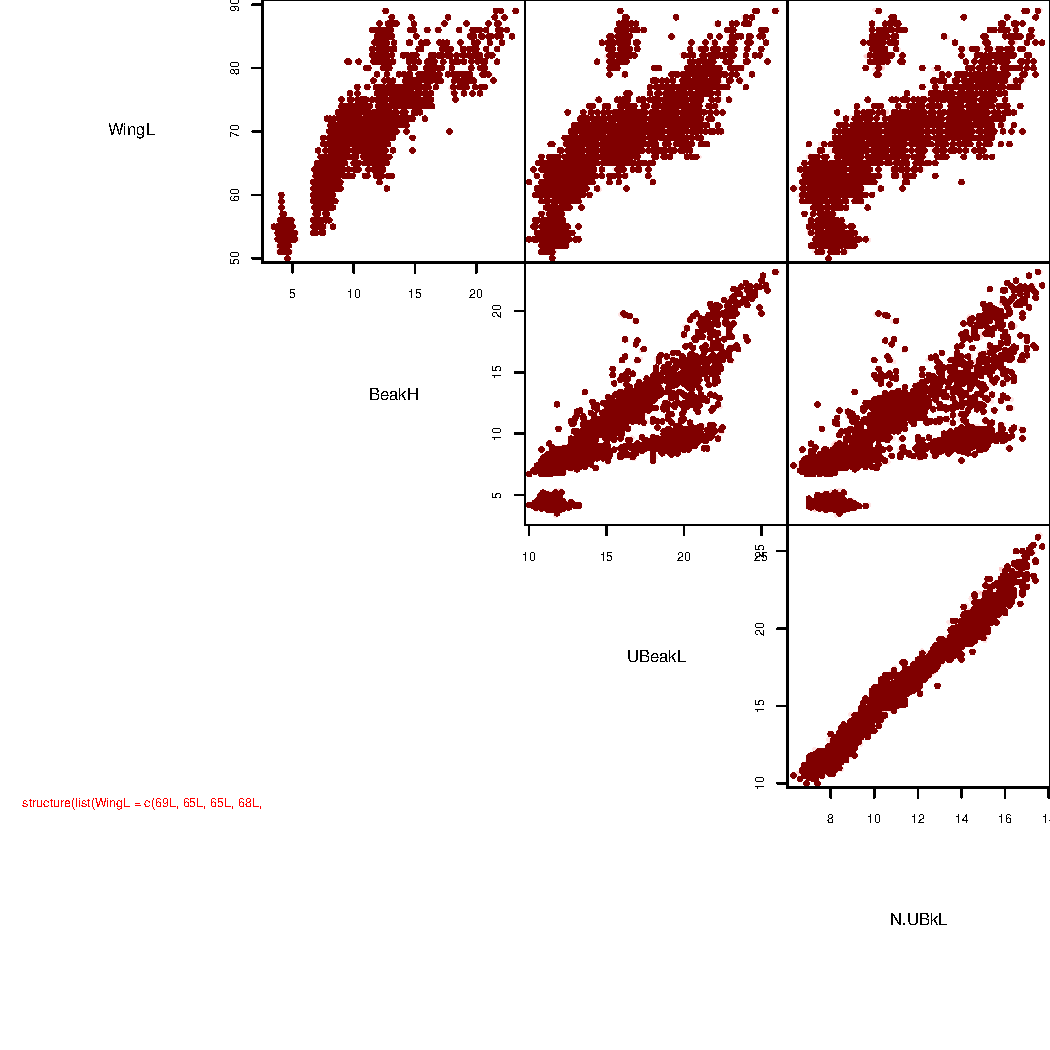
\includegraphics[width=\maxwidth]{figure/unnamed-chunk-36} 

\end{knitrout}


Now, we can do the same analysis for each species.

\begin{knitrout}
\definecolor{shadecolor}{rgb}{0.969, 0.969, 0.969}\color{fgcolor}\begin{kframe}
\begin{alltt}
\hlstd{hv.list} \hlkwb{<-} \hlkwd{new}\hlstd{(}\hlstr{"HypervolumeList"}\hlstd{)}
\hlstd{hv.list2} \hlkwb{<-} \hlkwd{list}\hlstd{()}

\hlkwa{for} \hlstd{(i} \hlkwa{in} \hlnum{1}\hlopt{:}\hlkwd{length}\hlstd{(}\hlkwd{table}\hlstd{(sp.finch))) \{}
    \hlstd{hv.list2[[i]]} \hlkwb{<-} \hlkwd{hypervolume}\hlstd{(traits.finch.mice[sp.finch} \hlopt{==} \hlkwd{levels}\hlstd{(sp.finch)[i],}
        \hlstd{],} \hlkwc{reps} \hlstd{=} \hlnum{1000}\hlstd{,} \hlkwc{bandwidth} \hlstd{=} \hlnum{0.2}\hlstd{,} \hlkwc{verbose} \hlstd{= F,} \hlkwc{warnings} \hlstd{= F)}
\hlstd{\}}

\hlstd{hv.list}\hlopt{@}\hlkwc{HVList} \hlkwb{<-} \hlstd{hv.list2}
\hlkwd{require}\hlstd{(adegenet)}
\end{alltt}


{\ttfamily\noindent\itshape\color{messagecolor}{\#\# Loading required package: adegenet\\\#\#\ \ \ \ ==========================\\\#\#\ \ \ \  adegenet 1.4-1 is loaded\\\#\#\ \ \ \ ==========================\\\#\# \\\#\#\ \ - to start, type '?adegenet'\\\#\#\ \ - to browse adegenet website, type 'adegenetWeb()'\\\#\#\ \ - to post questions/comments: adegenet-forum@lists.r-forge.r-project.org}}\begin{alltt}
\hlstd{colorhv} \hlkwb{<-} \hlkwd{transp}\hlstd{(}\hlkwd{funky}\hlstd{(}\hlkwd{nlevels}\hlstd{(sp.finch)),} \hlkwc{alpha} \hlstd{=} \hlnum{0.8}\hlstd{)}

\hlkwd{plot}\hlstd{(hv.list,} \hlkwc{colors} \hlstd{= colorhv,} \hlkwc{darkfactor} \hlstd{=} \hlnum{0.8}\hlstd{)}
\end{alltt}
\end{kframe}
\includegraphics[width=\maxwidth]{figure/unnamed-chunk-371} 
\begin{kframe}\begin{alltt}
\hlkwd{plot}\hlstd{(hv.list,} \hlkwc{colors} \hlstd{= colorhv,} \hlkwc{darkfactor} \hlstd{=} \hlnum{0.8}\hlstd{,} \hlkwc{showdata} \hlstd{= F,} \hlkwc{npmax} \hlstd{=} \hlnum{200}\hlstd{,}
    \hlkwc{cex.random} \hlstd{=} \hlnum{1}\hlstd{)}
\end{alltt}
\end{kframe}
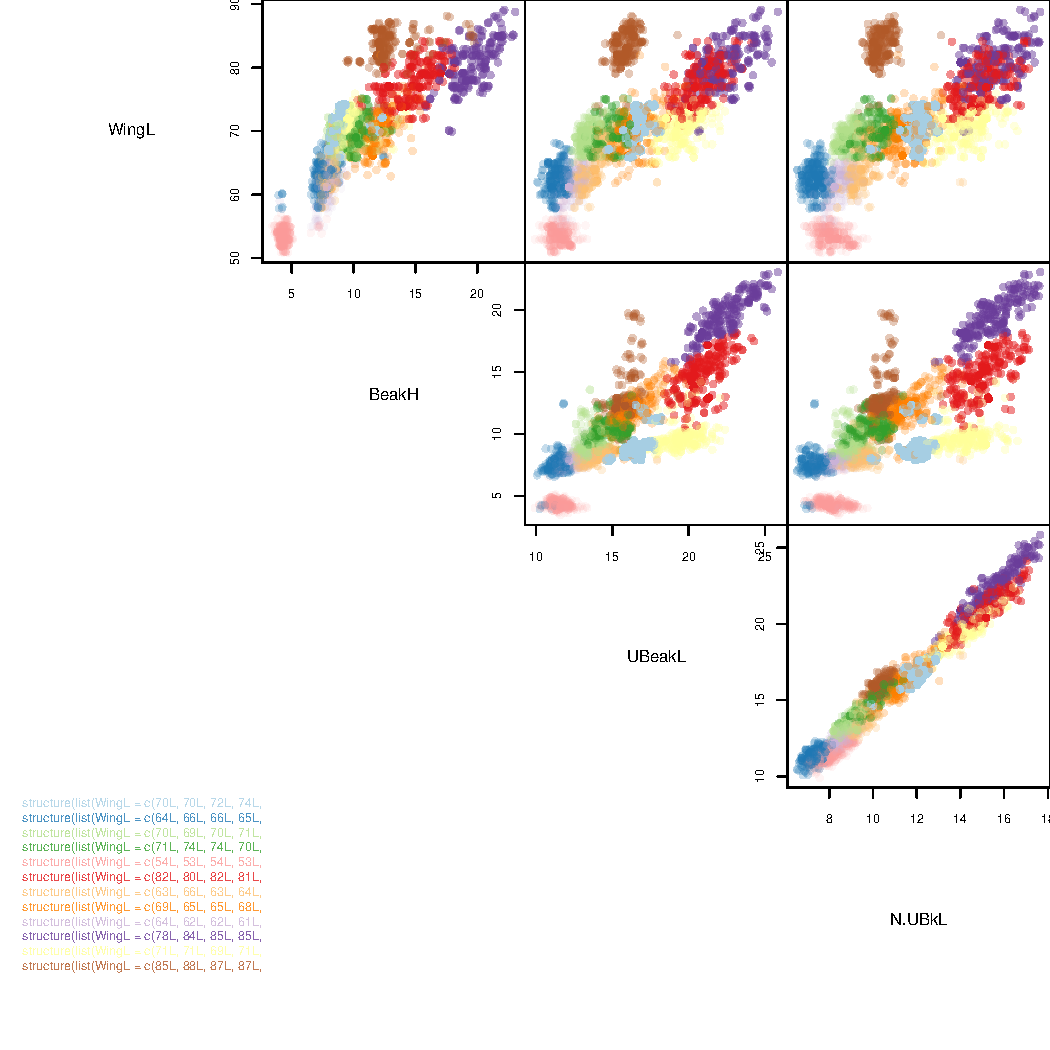
\includegraphics[width=\maxwidth]{figure/unnamed-chunk-372} 
\begin{kframe}\begin{alltt}
\hlkwd{summary}\hlstd{(hv.list)}
\end{alltt}
\begin{verbatim}
## Hypervolume
## 	Name: structure(list(WingL = c(70L, 70L, 72L, 74L, 74L, 72L, 73L, 73L, 
## 	Nr. of observations: 23
## 	Dimensionality: 4
## 	Volume: 0.588800
## 	Bandwidth: 0.2 0.2 0.2 0.2
## 	Quantile desired: 0.000000
## 	Quantile obtained: 0.000000
## 	Nr. of repetitions per point: 1000
## 	Number of random points: 14617
## Hypervolume
## 	Name: structure(list(WingL = c(64L, 66L, 66L, 65L, 65L, 63L, 63L, 62L, 
## 	Nr. of observations: 172
## 	Dimensionality: 4
## 	Volume: 3.512137
## 	Bandwidth: 0.2 0.2 0.2 0.2
## 	Quantile desired: 0.000000
## 	Quantile obtained: 0.000000
## 	Nr. of repetitions per point: 1000
## 	Number of random points: 91290
## Hypervolume
## 	Name: structure(list(WingL = c(70L, 69L, 70L, 71L, 72L, 69L, 71L, 68L, 
## 	Nr. of observations: 142
## 	Dimensionality: 4
## 	Volume: 3.062729
## 	Bandwidth: 0.2 0.2 0.2 0.2
## 	Quantile desired: 0.000000
## 	Quantile obtained: 0.000000
## 	Nr. of repetitions per point: 1000
## 	Number of random points: 78616
## Hypervolume
## 	Name: structure(list(WingL = c(71L, 74L, 74L, 70L, 68L, 70L, 70L, 66L, 
## 	Nr. of observations: 73
## 	Dimensionality: 4
## 	Volume: 1.727309
## 	Bandwidth: 0.2 0.2 0.2 0.2
## 	Quantile desired: 0.000000
## 	Quantile obtained: 0.000000
## 	Nr. of repetitions per point: 1000
## 	Number of random points: 43449
## Hypervolume
## 	Name: structure(list(WingL = c(54L, 53L, 54L, 53L, 54L, 53L, 53L, 53L, 
## 	Nr. of observations: 299
## 	Dimensionality: 4
## 	Volume: 4.132790
## 	Bandwidth: 0.2 0.2 0.2 0.2
## 	Quantile desired: 0.000000
## 	Quantile obtained: 0.000000
## 	Nr. of repetitions per point: 1000
## 	Number of random points: 114703
## Hypervolume
## 	Name: structure(list(WingL = c(82L, 80L, 82L, 81L, 82L, 80L, 84L, 83L, 
## 	Nr. of observations: 206
## 	Dimensionality: 4
## 	Volume: 5.100971
## 	Bandwidth: 0.2 0.2 0.2 0.2
## 	Quantile desired: 0.000000
## 	Quantile obtained: 0.000000
## 	Nr. of repetitions per point: 1000
## 	Number of random points: 127193
## Hypervolume
## 	Name: structure(list(WingL = c(63L, 66L, 63L, 64L, 63L, 61L, 62L, 65L, 
## 	Nr. of observations: 125
## 	Dimensionality: 4
## 	Volume: 2.758810
## 	Bandwidth: 0.2 0.2 0.2 0.2
## 	Quantile desired: 0.000000
## 	Quantile obtained: 0.000000
## 	Nr. of repetitions per point: 1000
## 	Number of random points: 70621
## Hypervolume
## 	Name: structure(list(WingL = c(69L, 65L, 65L, 68L, 66L, 68L, 67L, 69L, 
## 	Nr. of observations: 548
## 	Dimensionality: 4
## 	Volume: 11.764025
## 	Bandwidth: 0.2 0.2 0.2 0.2
## 	Quantile desired: 0.000000
## 	Quantile obtained: 0.000000
## 	Nr. of repetitions per point: 1000
## 	Number of random points: 302230
## Hypervolume
## 	Name: structure(list(WingL = c(64L, 62L, 62L, 61L, 67L, 64L, 64L, 63L, 
## 	Nr. of observations: 386
## 	Dimensionality: 4
## 	Volume: 6.372158
## 	Bandwidth: 0.2 0.2 0.2 0.2
## 	Quantile desired: 0.000000
## 	Quantile obtained: 0.000000
## 	Nr. of repetitions per point: 1000
## 	Number of random points: 171917
## Hypervolume
## 	Name: structure(list(WingL = c(78L, 84L, 85L, 85L, 87L, 89L, 87L, 86L, 
## 	Nr. of observations: 126
## 	Dimensionality: 4
## 	Volume: 3.158656
## 	Bandwidth: 0.2 0.2 0.2 0.2
## 	Quantile desired: 0.000000
## 	Quantile obtained: 0.000000
## 	Nr. of repetitions per point: 1000
## 	Number of random points: 78485
## Hypervolume
## 	Name: structure(list(WingL = c(71L, 71L, 69L, 71L, 73L, 71L, 71L, 71L, 
## 	Nr. of observations: 284
## 	Dimensionality: 4
## 	Volume: 6.384687
## 	Bandwidth: 0.2 0.2 0.2 0.2
## 	Quantile desired: 0.000000
## 	Quantile obtained: 0.000000
## 	Nr. of repetitions per point: 1000
## 	Number of random points: 162478
## Hypervolume
## 	Name: structure(list(WingL = c(85L, 88L, 87L, 87L, 85L, 74L, 86L, 85L, 
## 	Nr. of observations: 129
## 	Dimensionality: 4
## 	Volume: 2.897190
## 	Bandwidth: 0.2 0.2 0.2 0.2
## 	Quantile desired: 0.000000
## 	Quantile obtained: 0.000000
## 	Nr. of repetitions per point: 1000
## 	Number of random points: 73579
\end{verbatim}
\end{kframe}
\end{knitrout}


The standard example of the hypervolume package also use finch data but at the species level.

\begin{knitrout}
\definecolor{shadecolor}{rgb}{0.969, 0.969, 0.969}\color{fgcolor}\begin{kframe}
\begin{alltt}
\hlkwd{demo}\hlstd{(}\hlstr{"finch"}\hlstd{,} \hlkwc{package} \hlstd{=} \hlstr{"hypervolume"}\hlstd{)}
\end{alltt}
\begin{verbatim}
## 
## 
## 	demo(finch)
## 	---- ~~~~~
## 
## > if (exists('doHypervolumeFinchDemo')==TRUE)
## + {
## +   data(finch)
## +   
## +   species_list = unique(finch$Species)
## +   num_species = length(species_list)
## +   
## +   hv_finches_list = new("HypervolumeList")
## +   hv_finches_list@HVList = vector(mode="list",length=num_species)
## +   
## +   # compute hypervolumes for each species
## +   for (i in 1:num_species)
## +   {
## +     this_species = subset(finch, Species==species_list[i])
## +     # keep the trait data
## +     this_species_log <- log10(this_species[,2:ncol(this_species)])
## +     # make a hypervolume using auto-bandwidth
## +     hv_finches_list@HVList[[i]] <- hypervolume(this_species_log, bandwidth=estimate_bandwidth(this_species_log),
## +                                                reps=10000, quantile=0, name=as.character(species_list[i]), warn=FALSE)
## +   }
## +   
## +   # compute all pairwise overlaps
## +   overlap = matrix(NA, nrow=num_species, ncol=num_species)
## +   dimnames(overlap)=list(species_list, species_list)
## +   for (i in 1:num_species)
## +   {
## +     for (j in i:num_species)
## +     {
## +       if (i!=j)
## +       {
## +         # compute set operations on each pair
## +         this_set = hypervolume_set(hv_finches_list@HVList[[i]], hv_finches_list@HVList[[j]],reduction_factor=0.5, check_memory=FALSE)
## +         # calculate a Sorensen overlap index (2 x shared volume / sum of |hv1| + |hv2|)
## +         overlap[i,j] = 2 * this_set@HVList$Intersection@Volume / (hv_finches_list@HVList[[i]]@Volume + hv_finches_list@HVList[[j]]@Volume)
## +       }
## +     }   
## +   }
## +   
## + 
## +   
## +   # show all hypervolumes
## +   plot(hv_finches_list,npmax=500,darkfactor=0.5,cex.legend=0.25,cex.names=0.75)
## +   
## +   # show pairwise overlaps - note that actually very few species overlap in nine dimensions
## +   op <- par(mar=c(10,10,1,1))
## +   image(x=1:nrow(overlap), y=1:nrow(overlap), z=overlap,axes=F,xlab='',ylab='',col=rainbow(5))
## +   box()
## +   axis(side=1, at=1:(length(dimnames(overlap)[[1]])),dimnames(overlap)[[1]],las=2,cex.axis=0.75)
## +   axis(side=2, at=1:(length(dimnames(overlap)[[2]])),dimnames(overlap)[[2]],las=1,cex.axis=0.75)
## +   par(op)
## +   
## +   rm(doHypervolumeFinchDemo)
## + } else
## + {
## +   message('Demo does not run by default to meet CRAN runtime requirements.')
## +   message('This demo requires approximately 3 minutes to run.')  
## +   message('To run the demo, type')
## +   message('\tdoHypervolumeFinchDemo=TRUE')
## +   message('\tdemo(finch)')
## +   message('at the R command line prompt.')
## + }
\end{verbatim}


{\ttfamily\noindent\itshape\color{messagecolor}{\#\# Demo does not run by default to meet CRAN runtime requirements.\\\#\# This demo requires approximately 3 minutes to run.\\\#\# To run the demo, type\\\#\# 	doHypervolumeFinchDemo=TRUE\\\#\# 	demo(finch)\\\#\# at the R command line prompt.}}\end{kframe}
\end{knitrout}



\begin{knitrout}
\definecolor{shadecolor}{rgb}{0.969, 0.969, 0.969}\color{fgcolor}\begin{kframe}
\begin{alltt}
\hlstd{hv.1} \hlkwb{<-} \hlkwd{com.index.multi}\hlstd{(traits.finch.mice,} \hlkwc{index} \hlstd{=} \hlkwd{c}\hlstd{(}\hlstr{"as.numeric(try(hypervolume(na.omit(x), reps=100, \textbackslash{}n                                  bandwidth=0.2, verbose=F, warnings=F)@Volume))"}\hlstd{),}
    \hlkwc{by.factor} \hlstd{=} \hlkwd{rep}\hlstd{(}\hlnum{1}\hlstd{,} \hlkwd{length}\hlstd{(n_sp_plot)),} \hlkwc{nullmodels} \hlstd{=} \hlkwd{c}\hlstd{(}\hlnum{2}\hlstd{,} \hlnum{2}\hlstd{),} \hlkwc{ind.plot} \hlstd{= ind.plot.finch,}
    \hlkwc{nperm} \hlstd{=} \hlnum{9}\hlstd{,} \hlkwc{sp} \hlstd{= sp.finch)}
\end{alltt}
\begin{verbatim}
## [1] "creating null models"
## [1] "nm.2 25 %"
## [1] "nm.2 50 %"
## [1] "nm.2 75 %"
## [1] "nm.2 100 %"
## [1] "calcul of null values using null models"
## [1] "as.numeric(try(hypervolume(na.omit(x), reps=100, \n                                  bandwidth=0.2, verbose=F, warnings=F)@Volume)) 100 %"
## [1] "calcul of observed values"
## [1] "100 %"
\end{verbatim}
\begin{alltt}
\hlstd{hv.2} \hlkwb{<-} \hlkwd{com.index.multi}\hlstd{(traits.finch.mice,} \hlkwc{index} \hlstd{=} \hlkwd{c}\hlstd{(}\hlstr{"as.numeric(try(hypervolume(na.omit(x), reps=100, \textbackslash{}n                                  bandwidth=0.2, verbose=F, warnings=F)@Volume))"}\hlstd{),}
    \hlkwc{by.factor} \hlstd{= n_sp_plot,} \hlkwc{nullmodels} \hlstd{=} \hlkwd{c}\hlstd{(}\hlnum{2}\hlstd{,} \hlnum{2}\hlstd{),} \hlkwc{ind.plot} \hlstd{= ind.plot.finch,}
    \hlkwc{nperm} \hlstd{=} \hlnum{9}\hlstd{,} \hlkwc{sp} \hlstd{= sp.finch)}
\end{alltt}
\begin{verbatim}
## [1] "creating null models"
## [1] "nm.2 25 %"
## [1] "nm.2 50 %"
## [1] "nm.2 75 %"
## [1] "nm.2 100 %"
## [1] "calcul of null values using null models"
## [1] "as.numeric(try(hypervolume(na.omit(x), reps=100, \n                                  bandwidth=0.2, verbose=F, warnings=F)@Volume)) 100 %"
## [1] "calcul of observed values"
## [1] "100 %"
\end{verbatim}
\begin{alltt}
\hlstd{hv.3} \hlkwb{<-} \hlkwd{com.index.multi}\hlstd{(traits.finch.mice,} \hlkwc{index} \hlstd{=} \hlkwd{c}\hlstd{(}\hlstr{"as.numeric(try(hypervolume(na.omit(x), reps=100,\textbackslash{}n                                  bandwidth=0.2, verbose=F, warnings=F)@Volume))"}\hlstd{),}
    \hlkwc{by.factor} \hlstd{= ind.plot.finch,} \hlkwc{nullmodels} \hlstd{=} \hlkwd{c}\hlstd{(}\hlnum{2}\hlstd{,} \hlnum{2}\hlstd{),} \hlkwc{ind.plot} \hlstd{= ind.plot.finch,}
    \hlkwc{nperm} \hlstd{=} \hlnum{9}\hlstd{,} \hlkwc{sp} \hlstd{= sp.finch)}
\end{alltt}
\begin{verbatim}
## [1] "creating null models"
## [1] "nm.2 25 %"
## [1] "nm.2 50 %"
## [1] "nm.2 75 %"
## [1] "nm.2 100 %"
## [1] "calcul of null values using null models"
## [1] "as.numeric(try(hypervolume(na.omit(x), reps=100,\n                                  bandwidth=0.2, verbose=F, warnings=F)@Volume)) 100 %"
## [1] "calcul of observed values"
## [1] "100 %"
\end{verbatim}
\begin{alltt}
\hlstd{hv.4} \hlkwb{<-} \hlkwd{com.index.multi}\hlstd{(traits.finch.mice,} \hlkwc{index} \hlstd{=} \hlkwd{c}\hlstd{(}\hlstr{"as.numeric(try(hypervolume(na.omit(x), reps=100, \textbackslash{}n                                  bandwidth=0.2, verbose=F, warnings=F)@Volume))"}\hlstd{),}
    \hlkwc{by.factor} \hlstd{= sp.finch,} \hlkwc{nullmodels} \hlstd{=} \hlkwd{c}\hlstd{(}\hlnum{2}\hlstd{,} \hlnum{2}\hlstd{),} \hlkwc{ind.plot} \hlstd{= ind.plot.finch,} \hlkwc{nperm} \hlstd{=} \hlnum{9}\hlstd{,}
    \hlkwc{sp} \hlstd{= sp.finch)}
\end{alltt}
\begin{verbatim}
## [1] "creating null models"
## [1] "nm.2 25 %"
## [1] "nm.2 50 %"
## [1] "nm.2 75 %"
## [1] "nm.2 100 %"
## [1] "calcul of null values using null models"
## [1] "as.numeric(try(hypervolume(na.omit(x), reps=100, \n                                  bandwidth=0.2, verbose=F, warnings=F)@Volume)) 100 %"
## [1] "calcul of observed values"
## [1] "100 %"
\end{verbatim}
\begin{alltt}
\hlstd{list.ind.multi} \hlkwb{<-} \hlkwd{as.listofindex}\hlstd{(}\hlkwd{list}\hlstd{(hv.2, hv.3, hv.4))}

\hlstd{ses.list.multi} \hlkwb{<-} \hlkwd{ses.listofindex}\hlstd{(list.ind.multi)}
\end{alltt}
\end{kframe}
\end{knitrout}


\begin{knitrout}
\definecolor{shadecolor}{rgb}{0.969, 0.969, 0.969}\color{fgcolor}\begin{kframe}
\begin{alltt}
\hlkwd{plot}\hlstd{(list.ind.multi)}
\end{alltt}
\end{kframe}
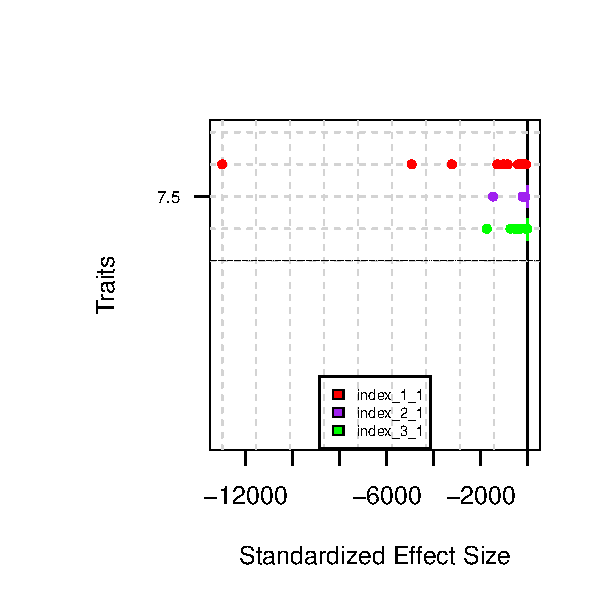
\includegraphics[width=\maxwidth]{figure/unnamed-chunk-401} 
\begin{kframe}\begin{alltt}
\hlkwd{plot}\hlstd{(list.ind.multi,} \hlkwc{xlim} \hlstd{=} \hlkwd{c}\hlstd{(}\hlopt{-}\hlnum{200}\hlstd{,} \hlnum{20}\hlstd{))}
\end{alltt}
\end{kframe}
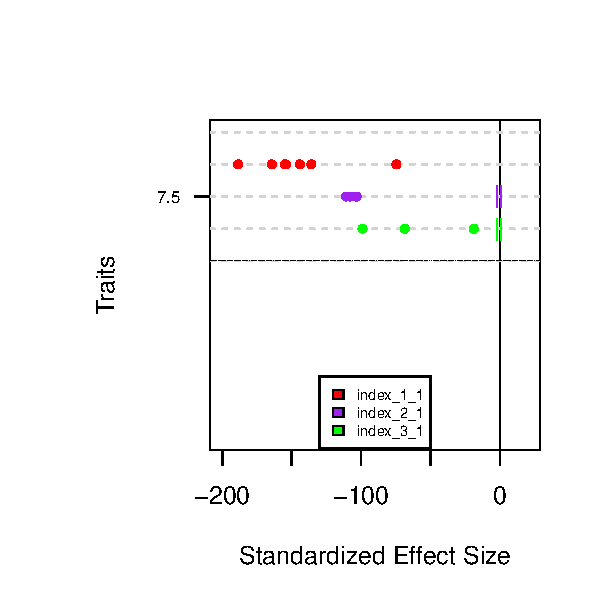
\includegraphics[width=\maxwidth]{figure/unnamed-chunk-402} 

\end{knitrout}



\section{Others graphics functions}

Using rasterVis to obtain more color schemes. 
\begin{knitrout}
\definecolor{shadecolor}{rgb}{0.969, 0.969, 0.969}\color{fgcolor}\begin{kframe}
\begin{alltt}
\hlkwd{require}\hlstd{(rasterVis)}
\hlcom{# Custom theme (from rasterVis package)}
\hlstd{my.theme} \hlkwb{<-} \hlkwd{BuRdTheme}\hlstd{()}
\hlcom{# Customize the colorkey}
\hlstd{my.ckey} \hlkwb{<-} \hlkwd{list}\hlstd{(}\hlkwc{col} \hlstd{= my.theme}\hlopt{$}\hlstd{regions}\hlopt{$}\hlstd{col)}
\end{alltt}
\end{kframe}
\end{knitrout}


Plot the p-value or the ses values using the function \code(levelplot).

\begin{knitrout}
\definecolor{shadecolor}{rgb}{0.969, 0.969, 0.969}\color{fgcolor}\begin{kframe}
\begin{alltt}
\hlkwd{levelplot}\hlstd{(}\hlkwd{t}\hlstd{(}\hlkwd{rbind}\hlstd{(res.finch}\hlopt{$}\hlstd{pval}\hlopt{$}\hlstd{T_IP.IC.inf, res.finch}\hlopt{$}\hlstd{pval}\hlopt{$}\hlstd{T_IC.IR.inf, res.finch}\hlopt{$}\hlstd{pval}\hlopt{$}\hlstd{T_PC.PR.inf)),}
    \hlkwc{colorkey} \hlstd{= my.ckey,} \hlkwc{par.settings} \hlstd{= my.theme,} \hlkwc{border} \hlstd{=} \hlstr{"black"}\hlstd{)}
\end{alltt}
\end{kframe}
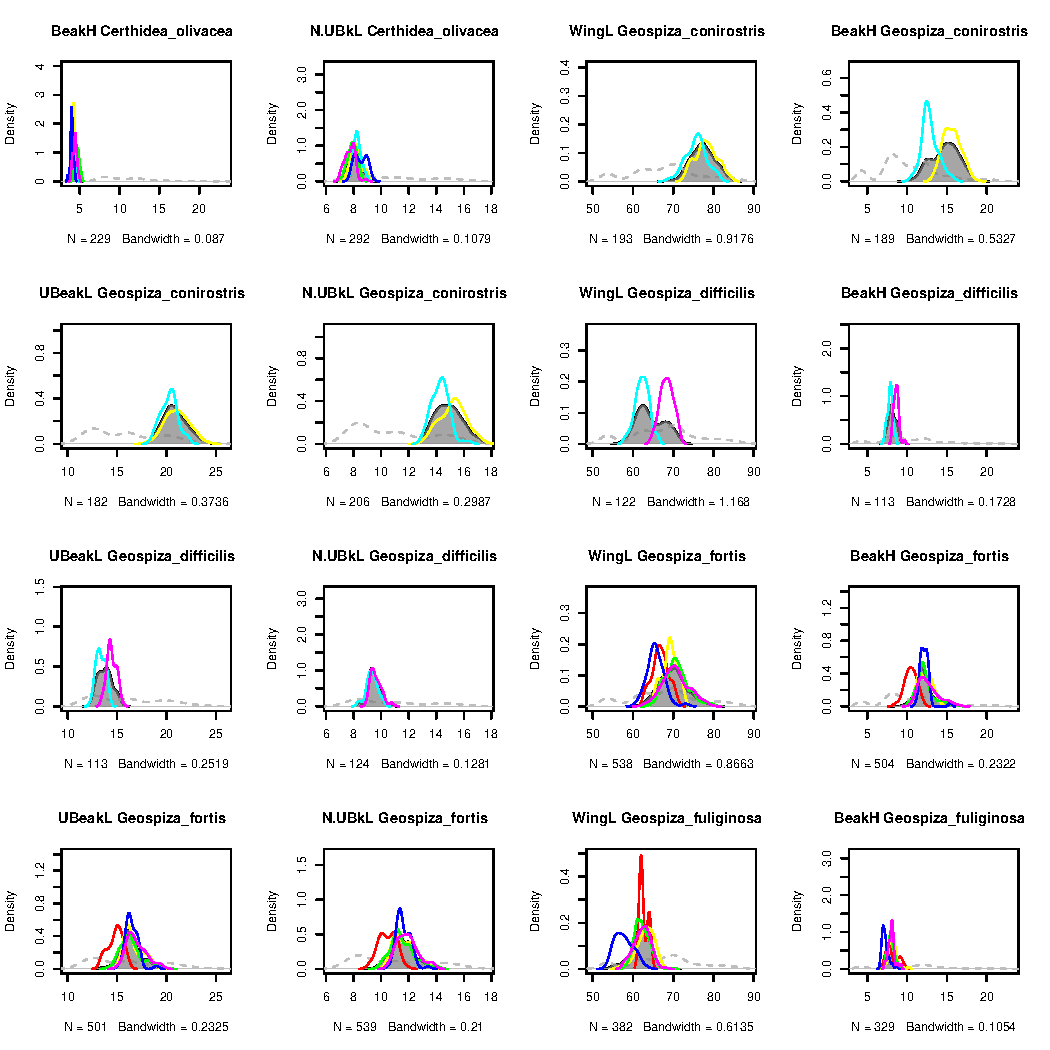
\includegraphics[width=\maxwidth]{figure/unnamed-chunk-42} 

\end{knitrout}



\begin{knitrout}
\definecolor{shadecolor}{rgb}{0.969, 0.969, 0.969}\color{fgcolor}\begin{kframe}
\begin{alltt}
\hlkwd{levelplot}\hlstd{(}\hlkwd{t}\hlstd{(}\hlkwd{ses}\hlstd{(res.finch}\hlopt{$}\hlstd{T_IP.IC, res.finch}\hlopt{$}\hlstd{T_IP.IC_nm)}\hlopt{$}\hlstd{ses),} \hlkwc{colorkey} \hlstd{= my.ckey,}
    \hlkwc{par.settings} \hlstd{= my.theme,} \hlkwc{border} \hlstd{=} \hlstr{"black"}\hlstd{)}
\end{alltt}
\end{kframe}
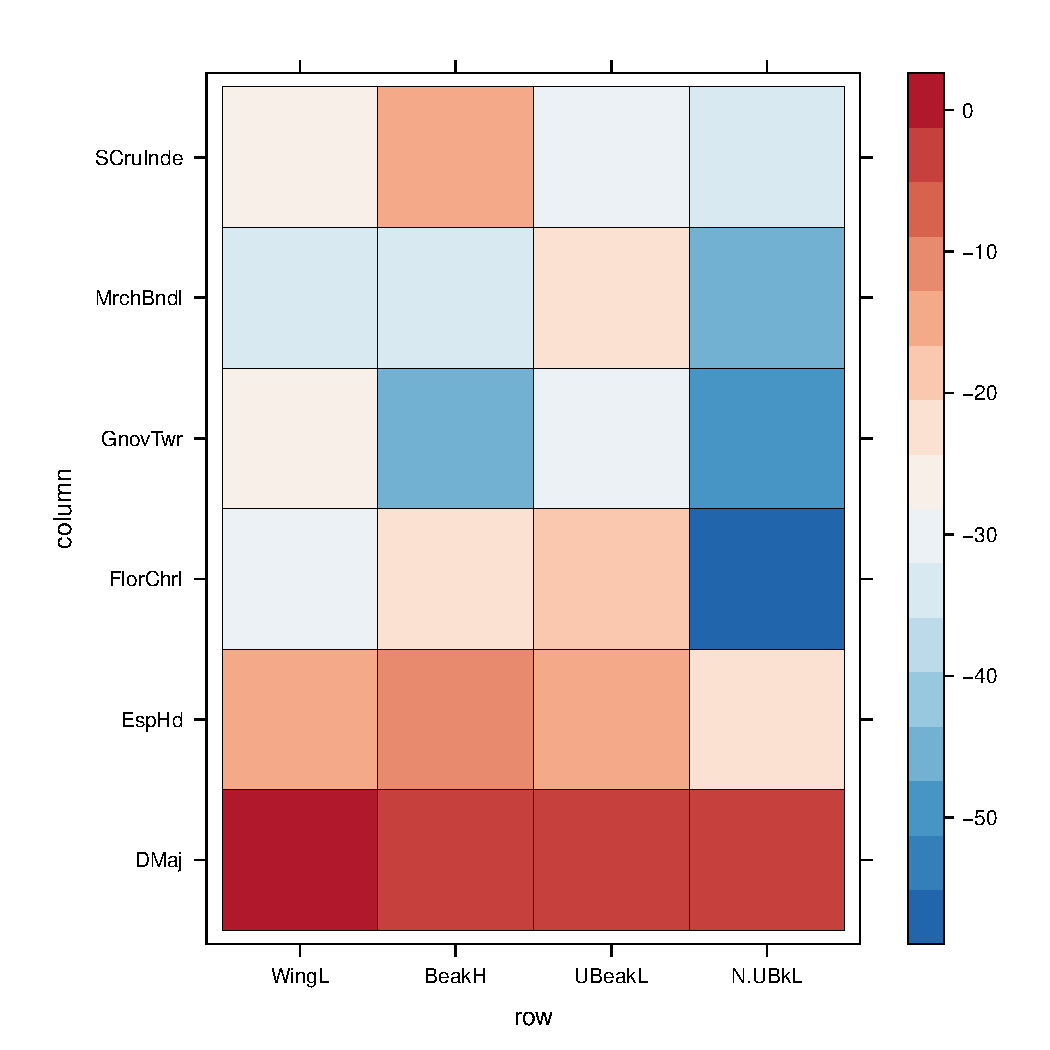
\includegraphics[width=\maxwidth]{figure/unnamed-chunk-431} 
\begin{kframe}\begin{alltt}
\hlkwd{levelplot}\hlstd{(}\hlkwd{cbind}\hlstd{(}\hlkwd{t}\hlstd{(}\hlkwd{ses}\hlstd{(res.finch}\hlopt{$}\hlstd{T_IP.IC, res.finch}\hlopt{$}\hlstd{T_IP.IC_nm)}\hlopt{$}\hlstd{ses),} \hlkwd{t}\hlstd{(}\hlkwd{ses}\hlstd{(res.finch}\hlopt{$}\hlstd{T_IC.IR,}
    \hlstd{res.finch}\hlopt{$}\hlstd{T_IP.IC_nm)}\hlopt{$}\hlstd{ses),} \hlkwd{t}\hlstd{(}\hlkwd{ses}\hlstd{(res.finch}\hlopt{$}\hlstd{T_PC.PR, res.finch}\hlopt{$}\hlstd{T_IP.IC_nm)}\hlopt{$}\hlstd{ses)),}
    \hlkwc{colorkey} \hlstd{= my.ckey,} \hlkwc{par.settings} \hlstd{= my.theme,} \hlkwc{border} \hlstd{=} \hlstr{"black"}\hlstd{)}
\end{alltt}
\end{kframe}
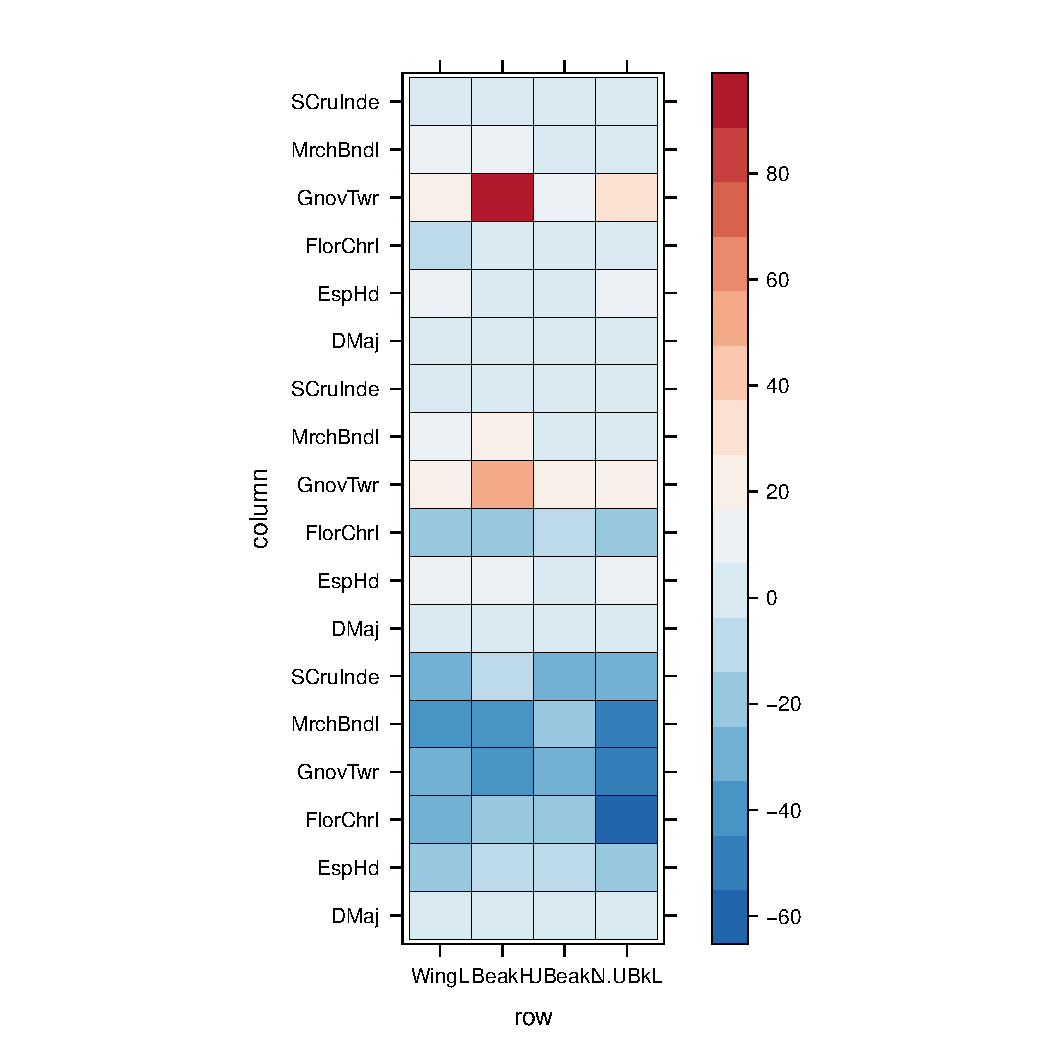
\includegraphics[width=\maxwidth]{figure/unnamed-chunk-432} 

\end{knitrout}


An other example using \code(ses.listofindex). The first plot represent "ses" values and the second one the result of a test with H0: observed index value are greater than what we can expect using the null model (alpha=2.5\%).

\begin{knitrout}
\definecolor{shadecolor}{rgb}{0.969, 0.969, 0.969}\color{fgcolor}\begin{kframe}
\begin{alltt}
\hlstd{ses.list} \hlkwb{<-} \hlkwd{ses.listofindex}\hlstd{(i.l1)}

\hlkwd{levelplot}\hlstd{(}\hlkwd{t}\hlstd{(}\hlkwd{rbind}\hlstd{(ses.list[[}\hlnum{1}\hlstd{]]}\hlopt{$}\hlstd{ses, ses.list[[}\hlnum{2}\hlstd{]]}\hlopt{$}\hlstd{ses, ses.list[[}\hlnum{3}\hlstd{]]}\hlopt{$}\hlstd{ses, ses.list[[}\hlnum{4}\hlstd{]]}\hlopt{$}\hlstd{ses)),}
    \hlkwc{colorkey} \hlstd{= my.ckey,} \hlkwc{par.settings} \hlstd{= my.theme,} \hlkwc{border} \hlstd{=} \hlstr{"black"}\hlstd{)}
\end{alltt}
\end{kframe}
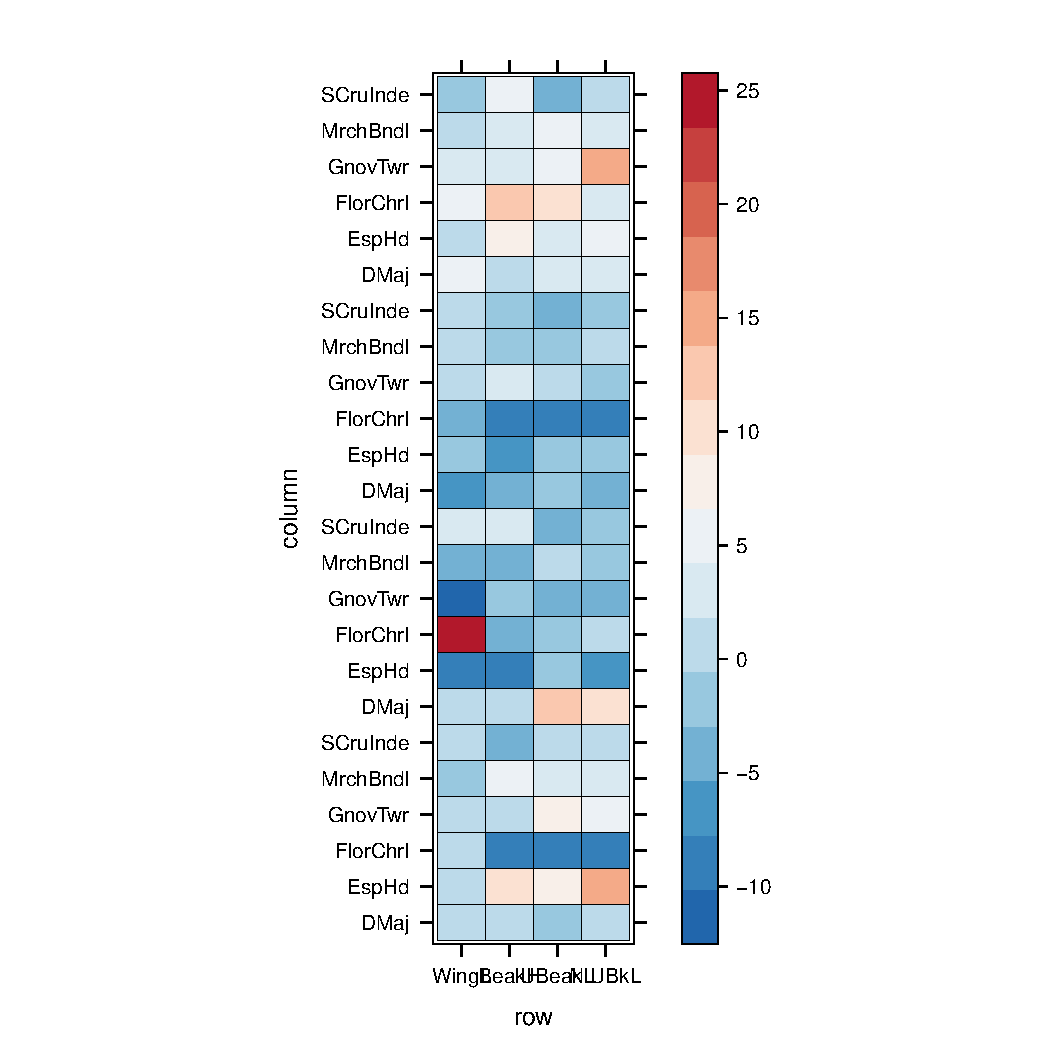
\includegraphics[width=\maxwidth]{figure/unnamed-chunk-441} 
\begin{kframe}\begin{alltt}
\hlkwd{levelplot}\hlstd{(}\hlkwd{t}\hlstd{(}\hlkwd{rbind}\hlstd{(ses.list[[}\hlnum{1}\hlstd{]]}\hlopt{$}\hlstd{ses} \hlopt{>} \hlstd{ses.list[[}\hlnum{1}\hlstd{]]}\hlopt{$}\hlstd{ses.sup, ses.list[[}\hlnum{2}\hlstd{]]}\hlopt{$}\hlstd{ses} \hlopt{>}
    \hlstd{ses.list[[}\hlnum{2}\hlstd{]]}\hlopt{$}\hlstd{ses.sup, ses.list[[}\hlnum{3}\hlstd{]]}\hlopt{$}\hlstd{ses} \hlopt{>} \hlstd{ses.list[[}\hlnum{3}\hlstd{]]}\hlopt{$}\hlstd{ses.sup, ses.list[[}\hlnum{4}\hlstd{]]}\hlopt{$}\hlstd{ses} \hlopt{>}
    \hlstd{ses.list[[}\hlnum{4}\hlstd{]]}\hlopt{$}\hlstd{ses.sup)),} \hlkwc{colorkey} \hlstd{= my.ckey,} \hlkwc{par.settings} \hlstd{= my.theme,} \hlkwc{border} \hlstd{=} \hlstr{"black"}\hlstd{)}
\end{alltt}
\end{kframe}
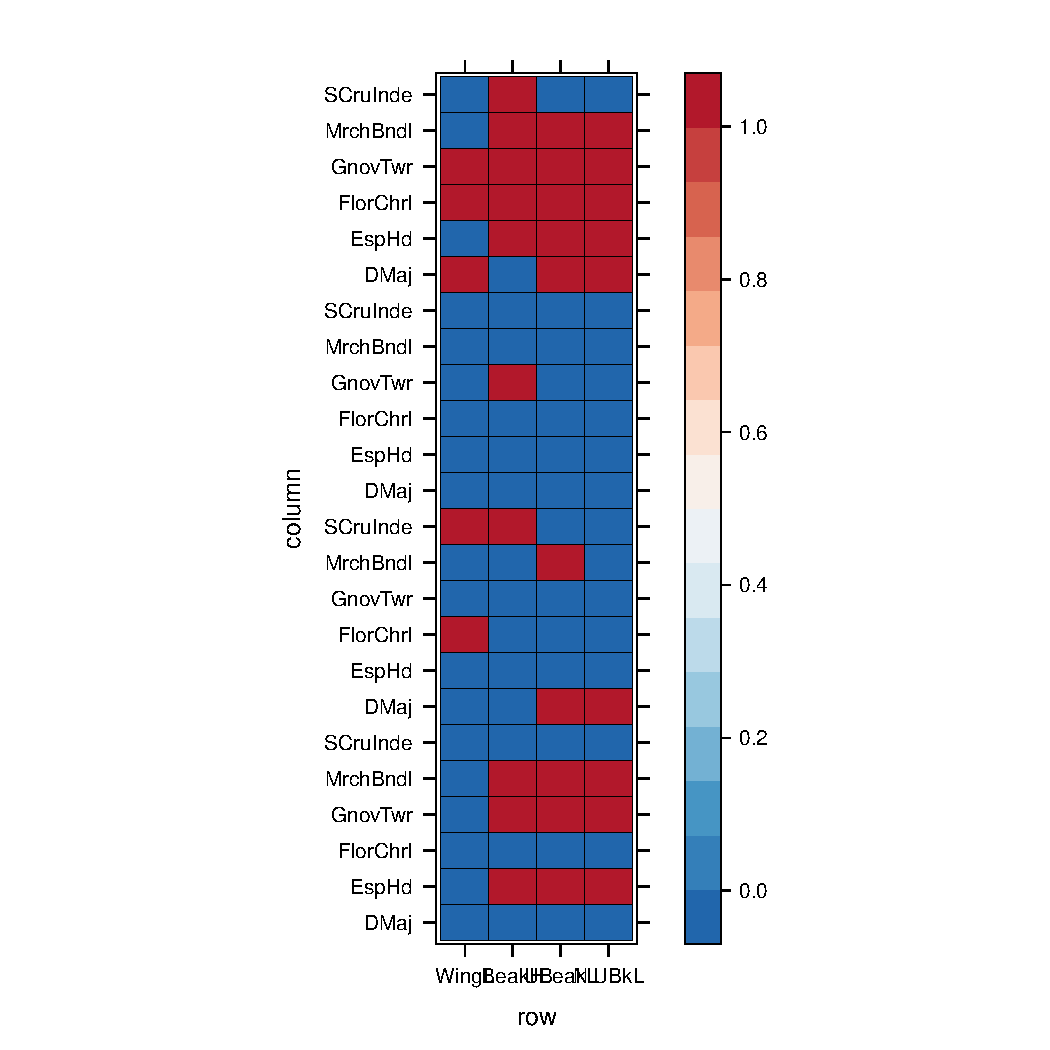
\includegraphics[width=\maxwidth]{figure/unnamed-chunk-442} 

\end{knitrout}



\begin{knitrout}
\definecolor{shadecolor}{rgb}{0.969, 0.969, 0.969}\color{fgcolor}\begin{kframe}
\begin{alltt}
\hlstd{obj1} \hlkwb{<-} \hlkwd{t}\hlstd{(}\hlkwd{rbind}\hlstd{(ses.list[[}\hlnum{1}\hlstd{]]}\hlopt{$}\hlstd{ses} \hlopt{>} \hlstd{ses.list[[}\hlnum{1}\hlstd{]]}\hlopt{$}\hlstd{ses.sup, ses.list[[}\hlnum{2}\hlstd{]]}\hlopt{$}\hlstd{ses} \hlopt{>}
    \hlstd{ses.list[[}\hlnum{2}\hlstd{]]}\hlopt{$}\hlstd{ses.sup, ses.list[[}\hlnum{3}\hlstd{]]}\hlopt{$}\hlstd{ses} \hlopt{>} \hlstd{ses.list[[}\hlnum{3}\hlstd{]]}\hlopt{$}\hlstd{ses.sup, ses.list[[}\hlnum{4}\hlstd{]]}\hlopt{$}\hlstd{ses} \hlopt{>}
    \hlstd{ses.list[[}\hlnum{4}\hlstd{]]}\hlopt{$}\hlstd{ses.sup))}

\hlstd{obj2} \hlkwb{<-} \hlkwd{t}\hlstd{(}\hlkwd{rbind}\hlstd{(ses.list[[}\hlnum{5}\hlstd{]]}\hlopt{$}\hlstd{ses} \hlopt{>} \hlstd{ses.list[[}\hlnum{5}\hlstd{]]}\hlopt{$}\hlstd{ses.sup, ses.list[[}\hlnum{6}\hlstd{]]}\hlopt{$}\hlstd{ses} \hlopt{>}
    \hlstd{ses.list[[}\hlnum{6}\hlstd{]]}\hlopt{$}\hlstd{ses.sup, ses.list[[}\hlnum{7}\hlstd{]]}\hlopt{$}\hlstd{ses} \hlopt{>} \hlstd{ses.list[[}\hlnum{7}\hlstd{]]}\hlopt{$}\hlstd{ses.sup, ses.list[[}\hlnum{8}\hlstd{]]}\hlopt{$}\hlstd{ses} \hlopt{>}
    \hlstd{ses.list[[}\hlnum{8}\hlstd{]]}\hlopt{$}\hlstd{ses.sup))}

\hlkwd{levelplot}\hlstd{(}\hlkwd{rbind}\hlstd{(obj1, obj2),} \hlkwc{colorkey} \hlstd{= my.ckey,} \hlkwc{par.settings} \hlstd{= my.theme,} \hlkwc{border} \hlstd{=} \hlstr{"black"}\hlstd{)}
\end{alltt}
\end{kframe}
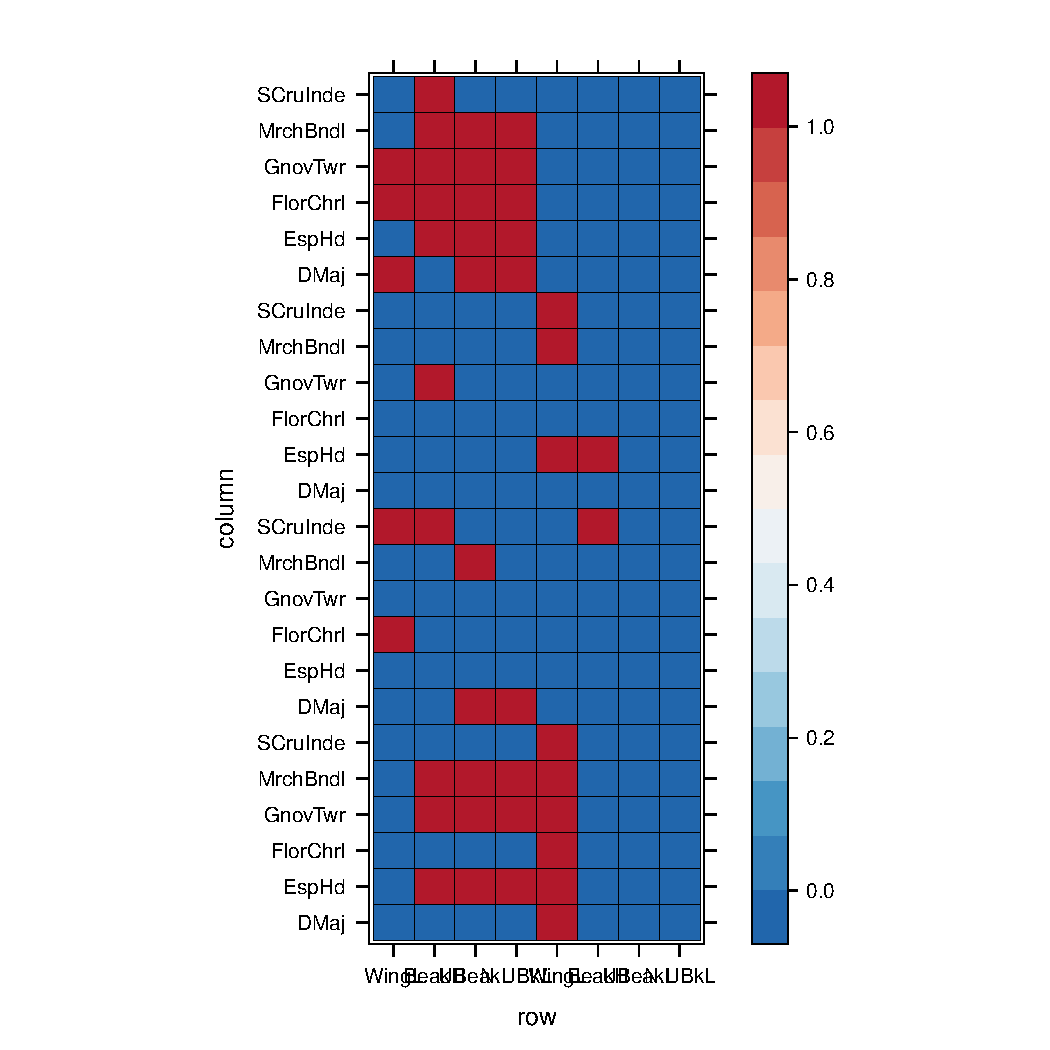
\includegraphics[width=\maxwidth]{figure/unnamed-chunk-451} 
\begin{kframe}\begin{alltt}
\hlstd{obj1.ses} \hlkwb{<-} \hlkwd{t}\hlstd{(}\hlkwd{rbind}\hlstd{(ses.list[[}\hlnum{1}\hlstd{]]}\hlopt{$}\hlstd{ses, ses.list[[}\hlnum{2}\hlstd{]]}\hlopt{$}\hlstd{ses, ses.list[[}\hlnum{3}\hlstd{]]}\hlopt{$}\hlstd{ses,}
    \hlstd{ses.list[[}\hlnum{4}\hlstd{]]}\hlopt{$}\hlstd{ses))}

\hlstd{obj2.ses} \hlkwb{<-} \hlkwd{t}\hlstd{(}\hlkwd{rbind}\hlstd{(ses.list[[}\hlnum{5}\hlstd{]]}\hlopt{$}\hlstd{ses, ses.list[[}\hlnum{6}\hlstd{]]}\hlopt{$}\hlstd{ses, ses.list[[}\hlnum{7}\hlstd{]]}\hlopt{$}\hlstd{ses,}
    \hlstd{ses.list[[}\hlnum{8}\hlstd{]]}\hlopt{$}\hlstd{ses))}

\hlkwd{levelplot}\hlstd{(}\hlkwd{rbind}\hlstd{(obj1.ses, obj2.ses),} \hlkwc{colorkey} \hlstd{= my.ckey,} \hlkwc{par.settings} \hlstd{= my.theme,}
    \hlkwc{border} \hlstd{=} \hlstr{"black"}\hlstd{)}
\end{alltt}
\end{kframe}
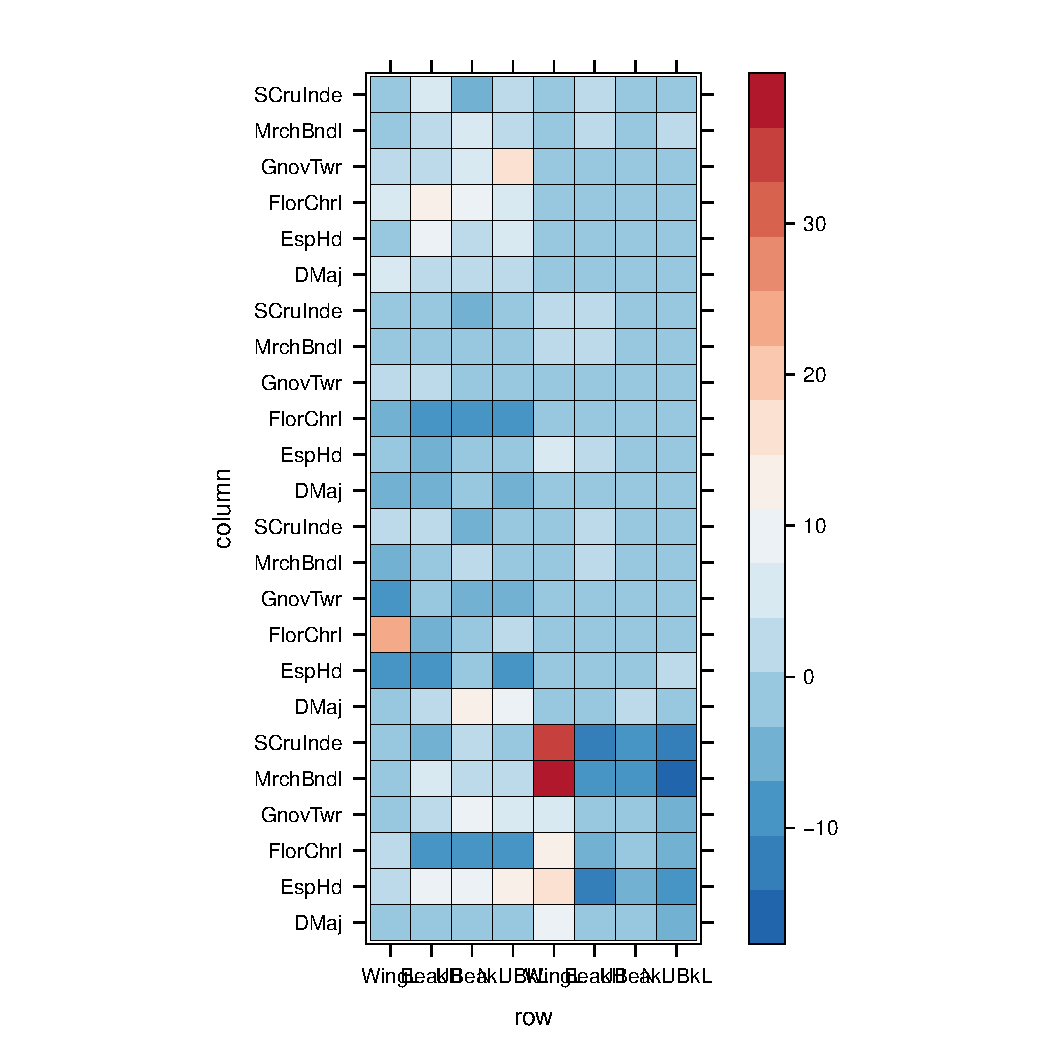
\includegraphics[width=\maxwidth]{figure/unnamed-chunk-452} 

\end{knitrout}



 
\begin{knitrout}
\definecolor{shadecolor}{rgb}{0.969, 0.969, 0.969}\color{fgcolor}\begin{kframe}
\begin{alltt}
\hlstd{ses.list.multi} \hlkwb{<-} \hlkwd{ses.listofindex}\hlstd{(list.ind.multi)}

\hlstd{ses.list.multi[[}\hlnum{1}\hlstd{]]} \hlkwb{<-} \hlkwd{lapply}\hlstd{(ses.list.multi[[}\hlnum{1}\hlstd{]],} \hlkwa{function}\hlstd{(}\hlkwc{x}\hlstd{) x[}\hlopt{!}\hlkwd{is.na}\hlstd{(ses.list.multi[[}\hlnum{1}\hlstd{]][[}\hlnum{2}\hlstd{]])])}
\hlstd{ses.list.multi[[}\hlnum{2}\hlstd{]]} \hlkwb{<-} \hlkwd{lapply}\hlstd{(ses.list.multi[[}\hlnum{2}\hlstd{]],} \hlkwa{function}\hlstd{(}\hlkwc{x}\hlstd{) x[}\hlopt{!}\hlkwd{is.na}\hlstd{(ses.list.multi[[}\hlnum{2}\hlstd{]][[}\hlnum{2}\hlstd{]])])}
\hlstd{ses.list.multi[[}\hlnum{3}\hlstd{]]} \hlkwb{<-} \hlkwd{lapply}\hlstd{(ses.list.multi[[}\hlnum{3}\hlstd{]],} \hlkwa{function}\hlstd{(}\hlkwc{x}\hlstd{) x[}\hlopt{!}\hlkwd{is.na}\hlstd{(ses.list.multi[[}\hlnum{3}\hlstd{]][[}\hlnum{2}\hlstd{]])])}

\hlkwd{levelplot}\hlstd{(}\hlkwd{t}\hlstd{(}\hlkwd{as.matrix}\hlstd{(ses.list.multi[[}\hlnum{1}\hlstd{]]}\hlopt{$}\hlstd{ses)),} \hlkwc{colorkey} \hlstd{= my.ckey,} \hlkwc{par.settings} \hlstd{= my.theme,}
    \hlkwc{border} \hlstd{=} \hlstr{"black"}\hlstd{)}
\end{alltt}
\end{kframe}

\includegraphics[width=\maxwidth]{figure/unnamed-chunk-461} 
\begin{kframe}\begin{alltt}
\hlkwd{levelplot}\hlstd{(}\hlkwd{t}\hlstd{(}\hlkwd{as.matrix}\hlstd{(ses.list.multi[[}\hlnum{2}\hlstd{]]}\hlopt{$}\hlstd{ses)),} \hlkwc{colorkey} \hlstd{= my.ckey,} \hlkwc{par.settings} \hlstd{= my.theme,}
    \hlkwc{border} \hlstd{=} \hlstr{"black"}\hlstd{)}
\end{alltt}
\end{kframe}

\includegraphics[width=\maxwidth]{figure/unnamed-chunk-462} 
\begin{kframe}\begin{alltt}
\hlkwd{levelplot}\hlstd{(}\hlkwd{t}\hlstd{(}\hlkwd{as.matrix}\hlstd{(ses.list.multi[[}\hlnum{3}\hlstd{]]}\hlopt{$}\hlstd{ses)),} \hlkwc{colorkey} \hlstd{= my.ckey,} \hlkwc{par.settings} \hlstd{= my.theme,}
    \hlkwc{border} \hlstd{=} \hlstr{"black"}\hlstd{)}
\end{alltt}
\end{kframe}

\includegraphics[width=\maxwidth]{figure/unnamed-chunk-463} 

\end{knitrout}


To finish, a multivariate analysis of 

\begin{knitrout}
\definecolor{shadecolor}{rgb}{0.969, 0.969, 0.969}\color{fgcolor}\begin{kframe}
\begin{alltt}
\hlkwd{require}\hlstd{(ade4)}
\hlkwd{require}\hlstd{(adegenet)}

\hlstd{matfordudi} \hlkwb{<-} \hlkwd{matrix}\hlstd{(}\hlkwc{nrow} \hlstd{=} \hlkwd{length}\hlstd{(}\hlkwd{colMeans}\hlstd{(ses.list[[i]]}\hlopt{$}\hlstd{ses)),} \hlkwc{ncol} \hlstd{=} \hlkwd{length}\hlstd{(}\hlkwd{names}\hlstd{(ses.list)))}
\end{alltt}


{\ttfamily\noindent\bfseries\color{errorcolor}{\#\# Error: indice hors limites}}\begin{alltt}
\hlkwa{for} \hlstd{(i} \hlkwa{in} \hlnum{1}\hlopt{:}\hlkwd{length}\hlstd{(}\hlkwd{names}\hlstd{(ses.list))) \{}
    \hlstd{matfordudi[, i]} \hlkwb{<-} \hlkwd{colMeans}\hlstd{(ses.list[[i]]}\hlopt{$}\hlstd{ses)}
\hlstd{\}}
\end{alltt}


{\ttfamily\noindent\bfseries\color{errorcolor}{\#\# Error: objet 'matfordudi' introuvable}}\begin{alltt}
\hlkwd{colnames}\hlstd{(matfordudi)} \hlkwb{<-} \hlkwd{names}\hlstd{(ses.list)}
\end{alltt}


{\ttfamily\noindent\bfseries\color{errorcolor}{\#\# Error: objet 'matfordudi' introuvable}}\begin{alltt}
\hlkwd{rownames}\hlstd{(matfordudi)} \hlkwb{<-} \hlkwd{colnames}\hlstd{(traits.finch)}
\end{alltt}


{\ttfamily\noindent\bfseries\color{errorcolor}{\#\# Error: objet 'matfordudi' introuvable}}\begin{alltt}
\hlstd{matfordudi2} \hlkwb{<-} \hlkwd{matrix}\hlstd{(}\hlkwc{nrow} \hlstd{=} \hlkwd{length}\hlstd{(}\hlkwd{as.vector}\hlstd{(ses.list[[}\hlnum{1}\hlstd{]]}\hlopt{$}\hlstd{ses)),} \hlkwc{ncol} \hlstd{=} \hlkwd{length}\hlstd{(}\hlkwd{names}\hlstd{(ses.list)))}
\hlkwa{for} \hlstd{(i} \hlkwa{in} \hlnum{1}\hlopt{:}\hlkwd{length}\hlstd{(}\hlkwd{names}\hlstd{(ses.list))) \{}
    \hlstd{matfordudi2[, i]} \hlkwb{<-} \hlkwd{as.vector}\hlstd{(ses.list[[i]]}\hlopt{$}\hlstd{ses)}
\hlstd{\}}
\hlkwd{colnames}\hlstd{(matfordudi2)} \hlkwb{<-} \hlkwd{names}\hlstd{(ses.list)}

\hlstd{res.dudi} \hlkwb{<-} \hlkwd{dudi.pca}\hlstd{(}\hlkwd{t}\hlstd{(matfordudi),} \hlkwc{scan} \hlstd{= F,} \hlkwc{nf} \hlstd{=} \hlnum{2}\hlstd{)}
\end{alltt}


{\ttfamily\noindent\bfseries\color{errorcolor}{\#\# Error: erreur d'évaluation de l'argument 'x' lors de la sélection d'une méthode pour la fonction 't' : Erreur : objet 'matfordudi' introuvable}}\begin{alltt}
\hlkwd{s.corcircle}\hlstd{(res.dudi}\hlopt{$}\hlstd{co)}
\end{alltt}


{\ttfamily\noindent\bfseries\color{errorcolor}{\#\# Error: objet 'res.dudi' introuvable}}\begin{alltt}
\hlkwd{s.label}\hlstd{(res.dudi}\hlopt{$}\hlstd{li,} \hlkwc{add.plot} \hlstd{= t)}
\end{alltt}


{\ttfamily\noindent\bfseries\color{errorcolor}{\#\# Error: objet 'res.dudi' introuvable}}\begin{alltt}
\hlstd{res.dudi2} \hlkwb{<-} \hlkwd{dudi.pca}\hlstd{(matfordudi2,} \hlkwc{scan} \hlstd{= F,} \hlkwc{nf} \hlstd{=} \hlnum{2}\hlstd{)}
\hlkwd{scatter}\hlstd{(res.dudi2)}
\end{alltt}
\end{kframe}
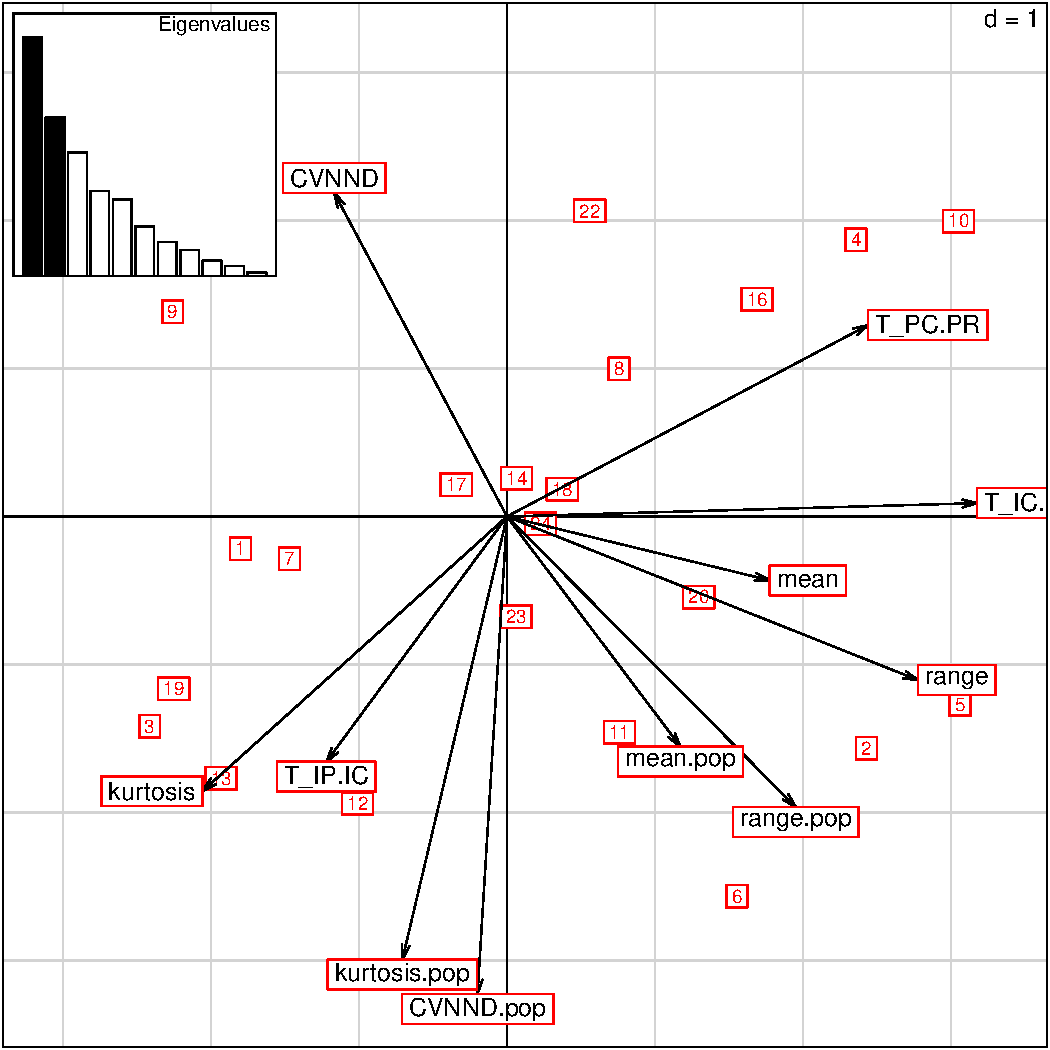
\includegraphics[width=\maxwidth]{figure/unnamed-chunk-471} 
\begin{kframe}\begin{alltt}
\hlkwd{s.corcircle}\hlstd{(res.dudi2}\hlopt{$}\hlstd{co)}
\end{alltt}
\end{kframe}
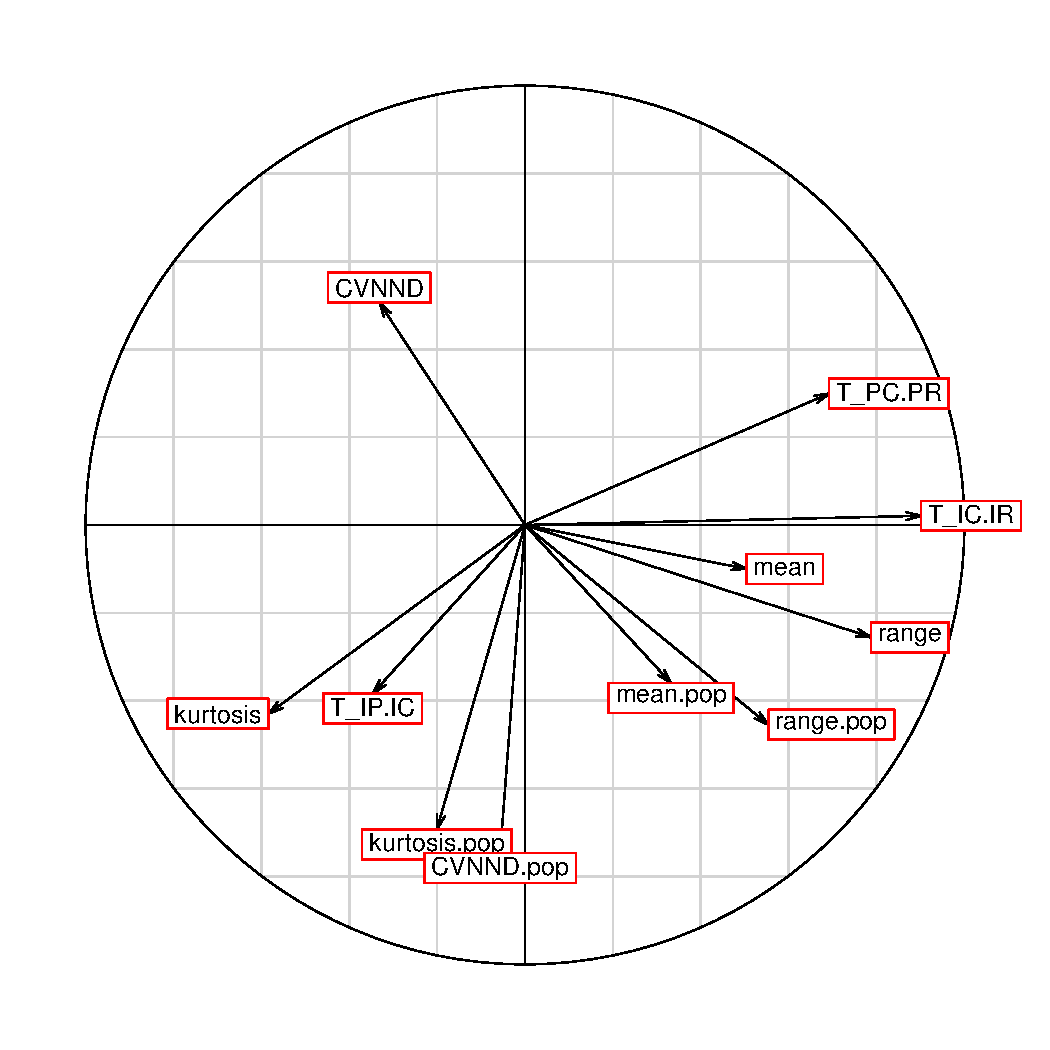
\includegraphics[width=\maxwidth]{figure/unnamed-chunk-472} 
\begin{kframe}\begin{alltt}
\hlkwd{s.class}\hlstd{(res.dudi2}\hlopt{$}\hlstd{li,} \hlkwd{as.factor}\hlstd{(}\hlkwd{c}\hlstd{(}\hlkwd{rep}\hlstd{(}\hlstr{"WingL"}\hlstd{,} \hlnum{6}\hlstd{),} \hlkwd{rep}\hlstd{(}\hlstr{"BeakH"}\hlstd{,} \hlnum{6}\hlstd{),} \hlkwd{rep}\hlstd{(}\hlstr{"UBeakL"}\hlstd{,}
    \hlnum{6}\hlstd{),} \hlkwd{rep}\hlstd{(}\hlstr{"N.UBkL"}\hlstd{,} \hlnum{6}\hlstd{))),} \hlkwc{col} \hlstd{=} \hlkwd{funky}\hlstd{(}\hlnum{4}\hlstd{))}
\end{alltt}
\end{kframe}
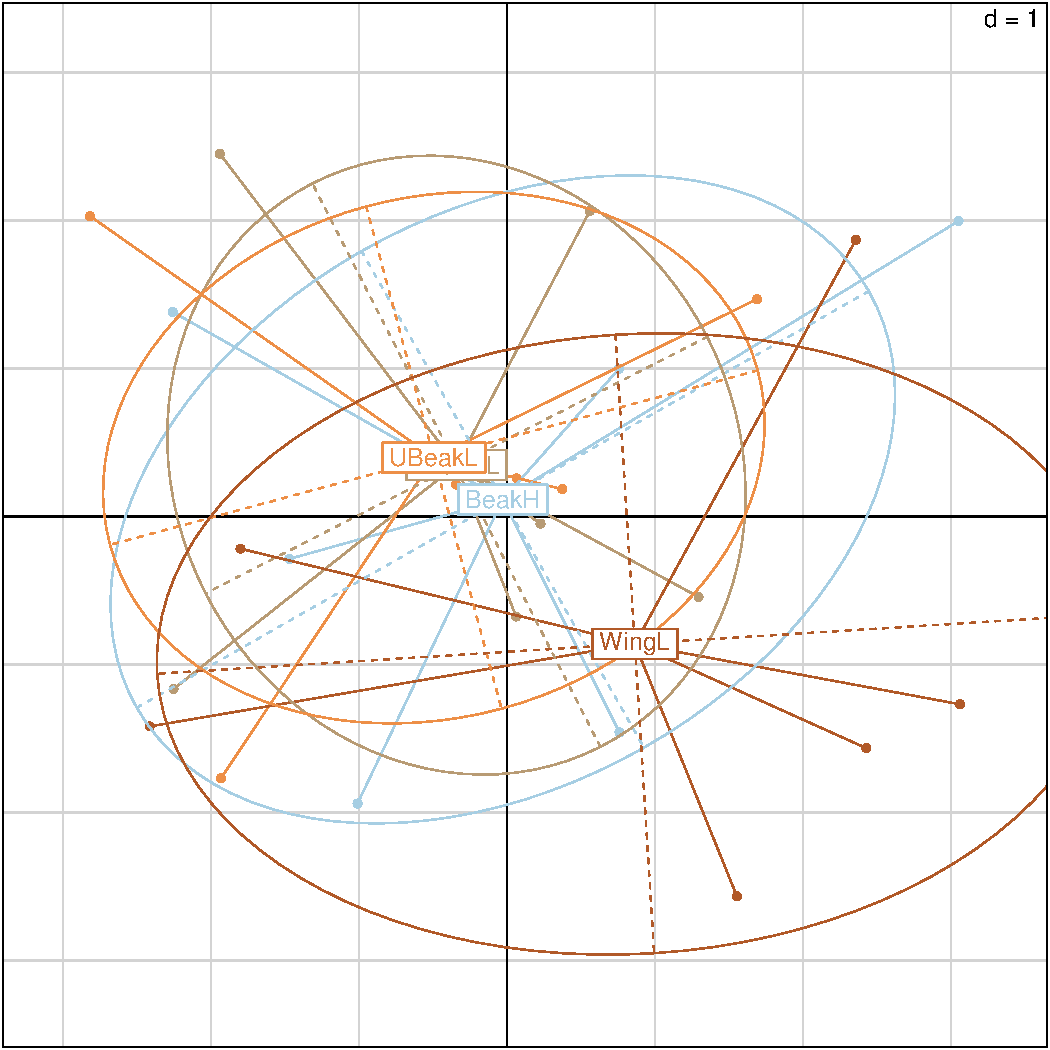
\includegraphics[width=\maxwidth]{figure/unnamed-chunk-473} 
\begin{kframe}\begin{alltt}
\hlkwd{s.class}\hlstd{(res.dudi2}\hlopt{$}\hlstd{li,} \hlkwd{as.factor}\hlstd{(}\hlkwd{rep}\hlstd{(}\hlkwd{c}\hlstd{(}\hlstr{"DMaj"}\hlstd{,} \hlstr{"EspHd"}\hlstd{,} \hlstr{"FlorChrl"}\hlstd{,} \hlstr{"GnovTwr"}\hlstd{,}
    \hlstr{"MrchBndl"}\hlstd{,} \hlstr{"SCruInde"}\hlstd{),} \hlnum{4}\hlstd{)),} \hlkwc{col} \hlstd{=} \hlkwd{funky}\hlstd{(}\hlnum{6}\hlstd{))}
\end{alltt}
\end{kframe}
\includegraphics[width=\maxwidth]{figure/unnamed-chunk-474} 

\end{knitrout}

 
\end{document}
